\documentclass[twoside]{book}

% Packages required by doxygen
\usepackage{fixltx2e}
\usepackage{calc}
\usepackage{doxygen}
\usepackage[export]{adjustbox} % also loads graphicx
\usepackage{graphicx}
\usepackage[utf8]{inputenc}
\usepackage{makeidx}
\usepackage{multicol}
\usepackage{multirow}
\PassOptionsToPackage{warn}{textcomp}
\usepackage{textcomp}
\usepackage[nointegrals]{wasysym}
\usepackage[table]{xcolor}

% Font selection
\usepackage[T1]{fontenc}
\usepackage[scaled=.90]{helvet}
\usepackage{courier}
\usepackage{amssymb}
\usepackage{sectsty}
\renewcommand{\familydefault}{\sfdefault}
\allsectionsfont{%
  \fontseries{bc}\selectfont%
  \color{darkgray}%
}
\renewcommand{\DoxyLabelFont}{%
  \fontseries{bc}\selectfont%
  \color{darkgray}%
}
\newcommand{\+}{\discretionary{\mbox{\scriptsize$\hookleftarrow$}}{}{}}

% Page & text layout
\usepackage{geometry}
\geometry{%
  a4paper,%
  top=2.5cm,%
  bottom=2.5cm,%
  left=2.5cm,%
  right=2.5cm%
}
\tolerance=750
\hfuzz=15pt
\hbadness=750
\setlength{\emergencystretch}{15pt}
\setlength{\parindent}{0cm}
\setlength{\parskip}{3ex plus 2ex minus 2ex}
\makeatletter
\renewcommand{\paragraph}{%
  \@startsection{paragraph}{4}{0ex}{-1.0ex}{1.0ex}{%
    \normalfont\normalsize\bfseries\SS@parafont%
  }%
}
\renewcommand{\subparagraph}{%
  \@startsection{subparagraph}{5}{0ex}{-1.0ex}{1.0ex}{%
    \normalfont\normalsize\bfseries\SS@subparafont%
  }%
}
\makeatother

% Headers & footers
\usepackage{fancyhdr}
\pagestyle{fancyplain}
\fancyhead[LE]{\fancyplain{}{\bfseries\thepage}}
\fancyhead[CE]{\fancyplain{}{}}
\fancyhead[RE]{\fancyplain{}{\bfseries\leftmark}}
\fancyhead[LO]{\fancyplain{}{\bfseries\rightmark}}
\fancyhead[CO]{\fancyplain{}{}}
\fancyhead[RO]{\fancyplain{}{\bfseries\thepage}}
\fancyfoot[LE]{\fancyplain{}{}}
\fancyfoot[CE]{\fancyplain{}{}}
\fancyfoot[RE]{\fancyplain{}{\bfseries\scriptsize Generated by Doxygen }}
\fancyfoot[LO]{\fancyplain{}{\bfseries\scriptsize Generated by Doxygen }}
\fancyfoot[CO]{\fancyplain{}{}}
\fancyfoot[RO]{\fancyplain{}{}}
\renewcommand{\footrulewidth}{0.4pt}
\renewcommand{\chaptermark}[1]{%
  \markboth{#1}{}%
}
\renewcommand{\sectionmark}[1]{%
  \markright{\thesection\ #1}%
}

% Indices & bibliography
\usepackage{natbib}
\usepackage[titles]{tocloft}
\setcounter{tocdepth}{3}
\setcounter{secnumdepth}{5}
\makeindex

% Hyperlinks (required, but should be loaded last)
\usepackage{ifpdf}
\ifpdf
  \usepackage[pdftex,pagebackref=true]{hyperref}
\else
  \usepackage[ps2pdf,pagebackref=true]{hyperref}
\fi
\hypersetup{%
  colorlinks=true,%
  linkcolor=blue,%
  citecolor=blue,%
  unicode%
}

% Custom commands
\newcommand{\clearemptydoublepage}{%
  \newpage{\pagestyle{empty}\cleardoublepage}%
}

\usepackage{caption}
\captionsetup{labelsep=space,justification=centering,font={bf},singlelinecheck=off,skip=4pt,position=top}

%===== C O N T E N T S =====

\begin{document}

% Titlepage & ToC
\hypersetup{pageanchor=false,
             bookmarksnumbered=true,
             pdfencoding=unicode
            }
\pagenumbering{roman}
\begin{titlepage}
\vspace*{7cm}
\begin{center}%
{\Large J\+S\+ON for C++ }\\
\vspace*{1cm}
{\large Generated by Doxygen 1.8.11}\\
\end{center}
\end{titlepage}
\clearemptydoublepage
\tableofcontents
\clearemptydoublepage
\pagenumbering{arabic}
\hypersetup{pageanchor=true}

%--- Begin generated contents ---
\chapter{Hierarchical Index}
\section{Class Hierarchy}
This inheritance list is sorted roughly, but not completely, alphabetically\+:\begin{DoxyCompactList}
\item \+\_\+\+\_\+ltr\+\_\+value\begin{DoxyCompactList}
\item \contentsline{section}{format}{\pageref{structformat}}{}
\end{DoxyCompactList}
\item exception\begin{DoxyCompactList}
\item \contentsline{section}{format\+:\+:json\+\_\+error}{\pageref{classformat_1_1json__error}}{}
\begin{DoxyCompactList}
\item \contentsline{section}{format\+:\+:json\+\_\+out\+\_\+of\+\_\+range}{\pageref{classformat_1_1json__out__of__range}}{}
\item \contentsline{section}{format\+:\+:json\+\_\+syntax\+\_\+error}{\pageref{classformat_1_1json__syntax__error}}{}
\end{DoxyCompactList}
\end{DoxyCompactList}
\item iterator\begin{DoxyCompactList}
\item \contentsline{section}{format\+:\+:value\+:\+:iterator$<$ Iterator, Category, T, Distance, Pointer, Reference $>$}{\pageref{classformat_1_1value_1_1iterator}}{}
\item \contentsline{section}{format\+:\+:value\+:\+:iterator$<$ element\+\_\+list\+:\+:iterator, std\+:\+:input\+\_\+iterator\+\_\+tag, value $\ast$, value $\ast$, value $\ast$, value \& $>$}{\pageref{classformat_1_1value_1_1iterator}}{}
\begin{DoxyCompactList}
\item \contentsline{section}{format\+:\+:array\+:\+:iterator}{\pageref{classformat_1_1array_1_1iterator}}{}
\end{DoxyCompactList}
\item \contentsline{section}{format\+:\+:value\+:\+:iterator$<$ member\+\_\+list\+:\+:iterator, std\+:\+:input\+\_\+iterator\+\_\+tag, std\+:\+:pair$<$ std\+:\+:string, value $\ast$ $>$, std\+:\+:pair$<$ std\+:\+:string, value $\ast$ $>$, value $\ast$, value \& $>$}{\pageref{classformat_1_1value_1_1iterator}}{}
\begin{DoxyCompactList}
\item \contentsline{section}{format\+:\+:object\+:\+:iterator}{\pageref{classformat_1_1object_1_1iterator}}{}
\end{DoxyCompactList}
\item \contentsline{section}{format\+:\+:value\+:\+:iterator$<$ value $\ast$, std\+:\+:input\+\_\+iterator\+\_\+tag, value $\ast$, value $\ast$, value $\ast$, value \& $>$}{\pageref{classformat_1_1value_1_1iterator}}{}
\begin{DoxyCompactList}
\item \contentsline{section}{format\+:\+:leaf\+:\+:iterator}{\pageref{classformat_1_1leaf_1_1iterator}}{}
\end{DoxyCompactList}
\end{DoxyCompactList}
\item \contentsline{section}{format\+:\+:value}{\pageref{classformat_1_1value}}{}
\begin{DoxyCompactList}
\item \contentsline{section}{format\+:\+:json}{\pageref{classformat_1_1json}}{}
\begin{DoxyCompactList}
\item \contentsline{section}{format\+:\+:array}{\pageref{classformat_1_1array}}{}
\item \contentsline{section}{format\+:\+:object}{\pageref{classformat_1_1object}}{}
\end{DoxyCompactList}
\item \contentsline{section}{format\+:\+:leaf}{\pageref{classformat_1_1leaf}}{}
\begin{DoxyCompactList}
\item \contentsline{section}{format\+:\+:boolean}{\pageref{classformat_1_1boolean}}{}
\item \contentsline{section}{format\+:\+:null}{\pageref{classformat_1_1null}}{}
\item \contentsline{section}{format\+:\+:number}{\pageref{classformat_1_1number}}{}
\item \contentsline{section}{format\+:\+:string}{\pageref{classformat_1_1string}}{}
\item \contentsline{section}{format\+:\+:undefined}{\pageref{classformat_1_1undefined}}{}
\begin{DoxyCompactList}
\item \contentsline{section}{format\+:\+:unique\+\_\+undefined}{\pageref{classformat_1_1unique__undefined}}{}
\begin{DoxyCompactList}
\item \contentsline{section}{format\+:\+:no\+\_\+value}{\pageref{classformat_1_1no__value}}{}
\end{DoxyCompactList}
\end{DoxyCompactList}
\end{DoxyCompactList}
\end{DoxyCompactList}
\end{DoxyCompactList}

\chapter{Class Index}
\section{Class List}
Here are the classes, structs, unions and interfaces with brief descriptions\+:\begin{DoxyCompactList}
\item\contentsline{section}{\hyperlink{classformat_1_1array}{format\+::array} \\*The array class }{\pageref{classformat_1_1array}}{}
\item\contentsline{section}{\hyperlink{classformat_1_1boolean}{format\+::boolean} \\*The boolean class }{\pageref{classformat_1_1boolean}}{}
\item\contentsline{section}{\hyperlink{structformat}{format} }{\pageref{structformat}}{}
\item\contentsline{section}{\hyperlink{classformat_1_1array_1_1iterator}{format\+::array\+::iterator} \\*The iterator class }{\pageref{classformat_1_1array_1_1iterator}}{}
\item\contentsline{section}{\hyperlink{classformat_1_1leaf_1_1iterator}{format\+::leaf\+::iterator} \\*The iterator class }{\pageref{classformat_1_1leaf_1_1iterator}}{}
\item\contentsline{section}{\hyperlink{classformat_1_1value_1_1iterator}{format\+::value\+::iterator$<$ Iterator, Category, T, Distance, Pointer, Reference $>$} \\*The iterator class }{\pageref{classformat_1_1value_1_1iterator}}{}
\item\contentsline{section}{\hyperlink{classformat_1_1object_1_1iterator}{format\+::object\+::iterator} \\*The iterator class }{\pageref{classformat_1_1object_1_1iterator}}{}
\item\contentsline{section}{\hyperlink{classformat_1_1json}{format\+::json} \\*The json class }{\pageref{classformat_1_1json}}{}
\item\contentsline{section}{\hyperlink{classformat_1_1json__error}{format\+::json\+\_\+error} \\*The J\+S\+O\+N\+\_\+\+Error class }{\pageref{classformat_1_1json__error}}{}
\item\contentsline{section}{\hyperlink{classformat_1_1json__out__of__range}{format\+::json\+\_\+out\+\_\+of\+\_\+range} \\*The J\+S\+O\+N\+\_\+\+Out\+\_\+\+Of\+\_\+\+Range class }{\pageref{classformat_1_1json__out__of__range}}{}
\item\contentsline{section}{\hyperlink{classformat_1_1json__syntax__error}{format\+::json\+\_\+syntax\+\_\+error} \\*The J\+S\+O\+N\+\_\+\+Syntax\+\_\+\+Error class }{\pageref{classformat_1_1json__syntax__error}}{}
\item\contentsline{section}{\hyperlink{classformat_1_1leaf}{format\+::leaf} \\*The leaf class }{\pageref{classformat_1_1leaf}}{}
\item\contentsline{section}{\hyperlink{classformat_1_1no__value}{format\+::no\+\_\+value} \\*The \hyperlink{classformat_1_1no__value}{no\+\_\+value} class }{\pageref{classformat_1_1no__value}}{}
\item\contentsline{section}{\hyperlink{classformat_1_1null}{format\+::null} \\*The null class }{\pageref{classformat_1_1null}}{}
\item\contentsline{section}{\hyperlink{classformat_1_1number}{format\+::number} \\*The number class }{\pageref{classformat_1_1number}}{}
\item\contentsline{section}{\hyperlink{classformat_1_1object}{format\+::object} \\*The object class }{\pageref{classformat_1_1object}}{}
\item\contentsline{section}{\hyperlink{classformat_1_1string}{format\+::string} \\*The string class }{\pageref{classformat_1_1string}}{}
\item\contentsline{section}{\hyperlink{classformat_1_1undefined}{format\+::undefined} \\*The undefined class }{\pageref{classformat_1_1undefined}}{}
\item\contentsline{section}{\hyperlink{classformat_1_1unique__undefined}{format\+::unique\+\_\+undefined} \\*The \hyperlink{classformat_1_1unique__undefined}{unique\+\_\+undefined} class }{\pageref{classformat_1_1unique__undefined}}{}
\item\contentsline{section}{\hyperlink{classformat_1_1value}{format\+::value} }{\pageref{classformat_1_1value}}{}
\end{DoxyCompactList}

\chapter{Class Documentation}
\hypertarget{classformat_1_1array}{}\section{format\+:\+:array Class Reference}
\label{classformat_1_1array}\index{format\+::array@{format\+::array}}


The array class.  




{\ttfamily \#include $<$json\+\_\+array.\+h$>$}



Inheritance diagram for format\+:\+:array\+:
\nopagebreak
\begin{figure}[H]
\begin{center}
\leavevmode
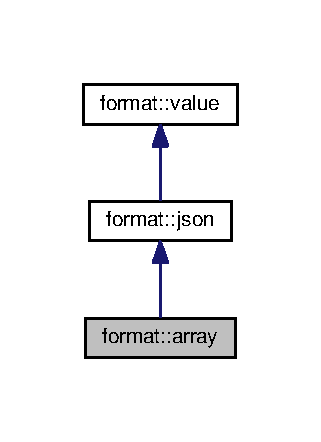
\includegraphics[width=154pt]{classformat_1_1array__inherit__graph}
\end{center}
\end{figure}


Collaboration diagram for format\+:\+:array\+:
\nopagebreak
\begin{figure}[H]
\begin{center}
\leavevmode
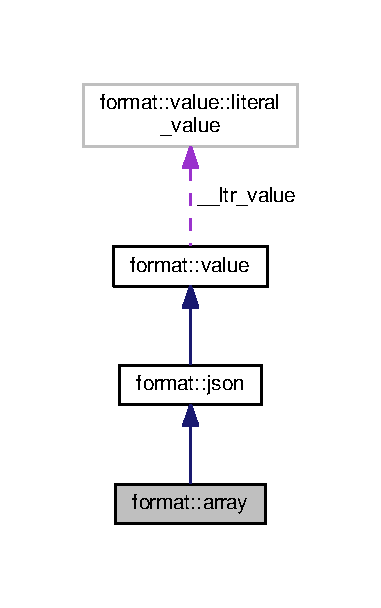
\includegraphics[width=183pt]{classformat_1_1array__coll__graph}
\end{center}
\end{figure}
\subsection*{Classes}
\begin{DoxyCompactItemize}
\item 
class \hyperlink{classformat_1_1array_1_1iterator}{iterator}
\begin{DoxyCompactList}\small\item\em The iterator class. \end{DoxyCompactList}\end{DoxyCompactItemize}
\subsection*{Public Types}
\begin{DoxyCompactItemize}
\item 
typedef std\+::vector$<$ \hyperlink{classformat_1_1value_aa6b85823936bf7b8ab78d3f8d443c00d}{value} $\ast$ $>$ \hyperlink{classformat_1_1array_a7167dd5489c3b9baeff3c937523f2a00}{element\+\_\+list}\hypertarget{classformat_1_1array_a7167dd5489c3b9baeff3c937523f2a00}{}\label{classformat_1_1array_a7167dd5489c3b9baeff3c937523f2a00}

\begin{DoxyCompactList}\small\item\em element\+\_\+list \end{DoxyCompactList}\end{DoxyCompactItemize}
\subsection*{Public Member Functions}
\begin{DoxyCompactItemize}
\item 
\hyperlink{classformat_1_1array_ab5ea2ac00086dd223936b1d18aef29fd}{array} ()\hypertarget{classformat_1_1array_ab5ea2ac00086dd223936b1d18aef29fd}{}\label{classformat_1_1array_ab5ea2ac00086dd223936b1d18aef29fd}

\begin{DoxyCompactList}\small\item\em array \end{DoxyCompactList}\item 
\hyperlink{classformat_1_1array_a17817a681d45278e357b4b0cabef3316}{array} (const wchar\+\_\+t $\ast$\hyperlink{classformat_1_1json}{json})
\begin{DoxyCompactList}\small\item\em array \end{DoxyCompactList}\item 
\hyperlink{classformat_1_1array_a305e57c21dfe05d3485a4b35d9123f73}{array} (std\+::initializer\+\_\+list$<$ \hyperlink{classformat_1_1value_aa6b85823936bf7b8ab78d3f8d443c00d}{value} $\ast$ $>$ il)
\begin{DoxyCompactList}\small\item\em array \end{DoxyCompactList}\item 
\hyperlink{classformat_1_1array_a3b00ec06a3a2e09905bceb7a1e9e2c3f}{array} (const \hyperlink{classformat_1_1array}{array} \&other)
\begin{DoxyCompactList}\small\item\em array \end{DoxyCompactList}\item 
virtual \hyperlink{classformat_1_1value_aa6b85823936bf7b8ab78d3f8d443c00d}{value} $\ast$ \hyperlink{classformat_1_1array_a456f53d9b5049e9af8d28b9588fc61c4}{clone} () const override
\begin{DoxyCompactList}\small\item\em clone \end{DoxyCompactList}\item 
virtual \hyperlink{classformat_1_1array_ac76e280a41976ee0e862d43118298968}{$\sim$array} () override\hypertarget{classformat_1_1array_ac76e280a41976ee0e862d43118298968}{}\label{classformat_1_1array_ac76e280a41976ee0e862d43118298968}

\begin{DoxyCompactList}\small\item\em $\sim$array \end{DoxyCompactList}\item 
virtual \hyperlink{classformat_1_1value_aa0334be06389a7b14af485fa0cd3aa21}{value\+\_\+t} \hyperlink{classformat_1_1array_a0fe16076f81ccc66e8208fe6dd4d2b1a}{type} () const noexceptoverride
\begin{DoxyCompactList}\small\item\em type \end{DoxyCompactList}\item 
virtual size\+\_\+t \hyperlink{classformat_1_1array_af15910f0535e266984f3f745efae5397}{length} () const noexceptoverride
\begin{DoxyCompactList}\small\item\em count \end{DoxyCompactList}\item 
\hyperlink{classformat_1_1value_aa6b85823936bf7b8ab78d3f8d443c00d}{value} \& \hyperlink{classformat_1_1array_a08ab9eaafc280dedec62b5b6f450164b}{operator=} (const \hyperlink{classformat_1_1array}{array} \&a)
\begin{DoxyCompactList}\small\item\em operator = \end{DoxyCompactList}\item 
virtual size\+\_\+t \hyperlink{classformat_1_1array_a579c320809545c627af0cbf9d8365080}{str\+\_\+length} () const noexceptoverride
\begin{DoxyCompactList}\small\item\em str\+\_\+length \end{DoxyCompactList}\item 
\hyperlink{classformat_1_1array_1_1iterator}{iterator} \hyperlink{classformat_1_1array_abbb0a5fbbcf3058b2eb34910e601aea0}{begin} ()
\begin{DoxyCompactList}\small\item\em begin \end{DoxyCompactList}\item 
\hyperlink{classformat_1_1array_1_1iterator}{iterator} \hyperlink{classformat_1_1array_aab3a5ba356998a7b15660f09ffd367ff}{end} ()
\begin{DoxyCompactList}\small\item\em end \end{DoxyCompactList}\end{DoxyCompactItemize}
\subsection*{Protected Member Functions}
\begin{DoxyCompactItemize}
\item 
\hyperlink{classformat_1_1array_a8f03c24948af29fa798f556a9689828c}{array} (\hyperlink{classformat_1_1json}{json} $\ast$\hyperlink{classformat_1_1value_a86c03ec8810bfd0d60ec49095120040d}{parent})
\begin{DoxyCompactList}\small\item\em array \end{DoxyCompactList}\item 
virtual const wchar\+\_\+t $\ast$ \hyperlink{classformat_1_1array_a7bd1454afcf365128e2a5db112b2895f}{\+\_\+parse} (const wchar\+\_\+t $\ast$\hyperlink{classformat_1_1json}{json}) override
\begin{DoxyCompactList}\small\item\em \+\_\+parse \end{DoxyCompactList}\item 
virtual \hyperlink{classformat_1_1value_aa6b85823936bf7b8ab78d3f8d443c00d}{value} \& \hyperlink{classformat_1_1array_a6e6822294f55273f657732d048aa38f8}{\+\_\+at} (const wchar\+\_\+t $\ast$\hyperlink{classformat_1_1value_ad4865e7984fc9f3b5ce7c17fd7ac740c}{key}) override
\begin{DoxyCompactList}\small\item\em \+\_\+at \end{DoxyCompactList}\item 
virtual \hyperlink{classformat_1_1value_aa6b85823936bf7b8ab78d3f8d443c00d}{value} \& \hyperlink{classformat_1_1array_a4407859f08e94c0d761dffd6eb4578f6}{\+\_\+assign} (\hyperlink{classformat_1_1value_aa6b85823936bf7b8ab78d3f8d443c00d}{value} $\ast$ov, \hyperlink{classformat_1_1value_aa6b85823936bf7b8ab78d3f8d443c00d}{value} $\ast$nv) override
\begin{DoxyCompactList}\small\item\em assign \end{DoxyCompactList}\item 
virtual \hyperlink{classformat_1_1value_aa6b85823936bf7b8ab78d3f8d443c00d}{value} \& \hyperlink{classformat_1_1array_a386fd4c0f2556459186db7f22df4128e}{\+\_\+at} (size\+\_\+t \hyperlink{classformat_1_1value_aaa429b28cc0edf5a3589b89a1820ad62}{index}) override
\begin{DoxyCompactList}\small\item\em \+\_\+at \end{DoxyCompactList}\item 
virtual void \hyperlink{classformat_1_1array_ac39a4a526a9101901f1712933793a4fd}{\+\_\+clear} ()\hypertarget{classformat_1_1array_ac39a4a526a9101901f1712933793a4fd}{}\label{classformat_1_1array_ac39a4a526a9101901f1712933793a4fd}

\begin{DoxyCompactList}\small\item\em \+\_\+clear \end{DoxyCompactList}\item 
virtual \hyperlink{classformat_1_1value_aa6b85823936bf7b8ab78d3f8d443c00d}{value} \& \hyperlink{classformat_1_1array_a543a2cf1adc8ff7f91eea7ea881c0247}{\+\_\+erase} (const \hyperlink{classformat_1_1value_aa6b85823936bf7b8ab78d3f8d443c00d}{value} \&v) noexceptoverride
\begin{DoxyCompactList}\small\item\em \+\_\+erase \end{DoxyCompactList}\item 
virtual \hyperlink{classformat_1_1value_aa6b85823936bf7b8ab78d3f8d443c00d}{value} $\ast$ \hyperlink{classformat_1_1array_abd0469398fdb7eed92ef3b785a94ae8f}{\+\_\+clone} (const \hyperlink{classformat_1_1value_aa6b85823936bf7b8ab78d3f8d443c00d}{value} \&other) override
\begin{DoxyCompactList}\small\item\em \+\_\+clone \end{DoxyCompactList}\item 
virtual const wchar\+\_\+t $\ast$ \hyperlink{classformat_1_1array_a3a8da80fceac963967b0d6d08a69ed18}{\+\_\+to\+\_\+string} (wchar\+\_\+t $\ast$offset=0) const override
\begin{DoxyCompactList}\small\item\em str\+\_\+value \end{DoxyCompactList}\end{DoxyCompactItemize}
\subsection*{Protected Attributes}
\begin{DoxyCompactItemize}
\item 
\hyperlink{classformat_1_1array_a7167dd5489c3b9baeff3c937523f2a00}{element\+\_\+list} \hyperlink{classformat_1_1array_a2d0d6853c95777dd971c713a1cfcf50c}{\+\_\+element\+\_\+list}\hypertarget{classformat_1_1array_a2d0d6853c95777dd971c713a1cfcf50c}{}\label{classformat_1_1array_a2d0d6853c95777dd971c713a1cfcf50c}

\begin{DoxyCompactList}\small\item\em \+\_\+element\+\_\+list \end{DoxyCompactList}\end{DoxyCompactItemize}
\subsection*{Friends}
\begin{DoxyCompactItemize}
\item 
\hyperlink{classformat_1_1array}{array} $\ast$ {\bfseries \+\_\+\+\_\+call\+\_\+array} (\hyperlink{classformat_1_1json}{json} $\ast$\hyperlink{classformat_1_1value_a86c03ec8810bfd0d60ec49095120040d}{parent})\hypertarget{classformat_1_1array_aca4fcdd614448f7dc0204b1c7a694577}{}\label{classformat_1_1array_aca4fcdd614448f7dc0204b1c7a694577}

\end{DoxyCompactItemize}
\subsection*{Additional Inherited Members}


\subsection{Detailed Description}
The array class. 

\subsection{Constructor \& Destructor Documentation}
\index{format\+::array@{format\+::array}!array@{array}}
\index{array@{array}!format\+::array@{format\+::array}}
\subsubsection[{\texorpdfstring{array(const wchar\+\_\+t $\ast$json)}{array(const wchar_t *json)}}]{\setlength{\rightskip}{0pt plus 5cm}format\+::array\+::array (
\begin{DoxyParamCaption}
\item[{const wchar\+\_\+t $\ast$}]{json}
\end{DoxyParamCaption}
)}\hypertarget{classformat_1_1array_a17817a681d45278e357b4b0cabef3316}{}\label{classformat_1_1array_a17817a681d45278e357b4b0cabef3316}


array 


\begin{DoxyParams}{Parameters}
{\em json} & \\
\hline
\end{DoxyParams}
\index{format\+::array@{format\+::array}!array@{array}}
\index{array@{array}!format\+::array@{format\+::array}}
\subsubsection[{\texorpdfstring{array(std\+::initializer\+\_\+list$<$ value $\ast$ $>$ il)}{array(std::initializer_list< value * > il)}}]{\setlength{\rightskip}{0pt plus 5cm}format\+::array\+::array (
\begin{DoxyParamCaption}
\item[{std\+::initializer\+\_\+list$<$ {\bf value} $\ast$ $>$}]{il}
\end{DoxyParamCaption}
)}\hypertarget{classformat_1_1array_a305e57c21dfe05d3485a4b35d9123f73}{}\label{classformat_1_1array_a305e57c21dfe05d3485a4b35d9123f73}


array 


\begin{DoxyParams}{Parameters}
{\em il} & \\
\hline
\end{DoxyParams}
\index{format\+::array@{format\+::array}!array@{array}}
\index{array@{array}!format\+::array@{format\+::array}}
\subsubsection[{\texorpdfstring{array(const array \&other)}{array(const array &other)}}]{\setlength{\rightskip}{0pt plus 5cm}format\+::array\+::array (
\begin{DoxyParamCaption}
\item[{const {\bf array} \&}]{other}
\end{DoxyParamCaption}
)}\hypertarget{classformat_1_1array_a3b00ec06a3a2e09905bceb7a1e9e2c3f}{}\label{classformat_1_1array_a3b00ec06a3a2e09905bceb7a1e9e2c3f}


array 


\begin{DoxyParams}{Parameters}
{\em other} & \\
\hline
\end{DoxyParams}
\index{format\+::array@{format\+::array}!array@{array}}
\index{array@{array}!format\+::array@{format\+::array}}
\subsubsection[{\texorpdfstring{array(json $\ast$parent)}{array(json *parent)}}]{\setlength{\rightskip}{0pt plus 5cm}format\+::array\+::array (
\begin{DoxyParamCaption}
\item[{{\bf json} $\ast$}]{parent}
\end{DoxyParamCaption}
)\hspace{0.3cm}{\ttfamily [protected]}}\hypertarget{classformat_1_1array_a8f03c24948af29fa798f556a9689828c}{}\label{classformat_1_1array_a8f03c24948af29fa798f556a9689828c}


array 


\begin{DoxyParams}{Parameters}
{\em parent} & \\
\hline
\end{DoxyParams}


\subsection{Member Function Documentation}
\index{format\+::array@{format\+::array}!\+\_\+assign@{\+\_\+assign}}
\index{\+\_\+assign@{\+\_\+assign}!format\+::array@{format\+::array}}
\subsubsection[{\texorpdfstring{\+\_\+assign(value $\ast$ov, value $\ast$nv) override}{_assign(value *ov, value *nv) override}}]{\setlength{\rightskip}{0pt plus 5cm}{\bf format\+::value} \& format\+::array\+::\+\_\+assign (
\begin{DoxyParamCaption}
\item[{{\bf value} $\ast$}]{ov, }
\item[{{\bf value} $\ast$}]{nv}
\end{DoxyParamCaption}
)\hspace{0.3cm}{\ttfamily [override]}, {\ttfamily [protected]}, {\ttfamily [virtual]}}\hypertarget{classformat_1_1array_a4407859f08e94c0d761dffd6eb4578f6}{}\label{classformat_1_1array_a4407859f08e94c0d761dffd6eb4578f6}


assign 


\begin{DoxyParams}{Parameters}
{\em ov} & \\
\hline
{\em nv} & \\
\hline
\end{DoxyParams}


Reimplemented from \hyperlink{classformat_1_1json_a331d385e55541671d431d5e5167e8c90}{format\+::json}.

\index{format\+::array@{format\+::array}!\+\_\+at@{\+\_\+at}}
\index{\+\_\+at@{\+\_\+at}!format\+::array@{format\+::array}}
\subsubsection[{\texorpdfstring{\+\_\+at(const wchar\+\_\+t $\ast$key) override}{_at(const wchar_t *key) override}}]{\setlength{\rightskip}{0pt plus 5cm}virtual {\bf value}\& format\+::array\+::\+\_\+at (
\begin{DoxyParamCaption}
\item[{const wchar\+\_\+t $\ast$}]{key}
\end{DoxyParamCaption}
)\hspace{0.3cm}{\ttfamily [inline]}, {\ttfamily [override]}, {\ttfamily [protected]}, {\ttfamily [virtual]}}\hypertarget{classformat_1_1array_a6e6822294f55273f657732d048aa38f8}{}\label{classformat_1_1array_a6e6822294f55273f657732d048aa38f8}


\+\_\+at 


\begin{DoxyParams}{Parameters}
{\em key} & \\
\hline
\end{DoxyParams}
\begin{DoxyReturn}{Returns}

\end{DoxyReturn}


Reimplemented from \hyperlink{classformat_1_1json_afcb78dfb597d7d609c66a4d5b6575082}{format\+::json}.

\index{format\+::array@{format\+::array}!\+\_\+at@{\+\_\+at}}
\index{\+\_\+at@{\+\_\+at}!format\+::array@{format\+::array}}
\subsubsection[{\texorpdfstring{\+\_\+at(size\+\_\+t index) override}{_at(size_t index) override}}]{\setlength{\rightskip}{0pt plus 5cm}{\bf format\+::value} \& format\+::array\+::\+\_\+at (
\begin{DoxyParamCaption}
\item[{size\+\_\+t}]{index}
\end{DoxyParamCaption}
)\hspace{0.3cm}{\ttfamily [override]}, {\ttfamily [protected]}, {\ttfamily [virtual]}}\hypertarget{classformat_1_1array_a386fd4c0f2556459186db7f22df4128e}{}\label{classformat_1_1array_a386fd4c0f2556459186db7f22df4128e}


\+\_\+at 


\begin{DoxyParams}{Parameters}
{\em index} & \\
\hline
\end{DoxyParams}
\begin{DoxyReturn}{Returns}

\end{DoxyReturn}


Reimplemented from \hyperlink{classformat_1_1json_a4a3924d5a112cda2bcee45ddf92a3d52}{format\+::json}.

\index{format\+::array@{format\+::array}!\+\_\+clone@{\+\_\+clone}}
\index{\+\_\+clone@{\+\_\+clone}!format\+::array@{format\+::array}}
\subsubsection[{\texorpdfstring{\+\_\+clone(const value \&other) override}{_clone(const value &other) override}}]{\setlength{\rightskip}{0pt plus 5cm}{\bf format\+::value} $\ast$ format\+::array\+::\+\_\+clone (
\begin{DoxyParamCaption}
\item[{const {\bf value} \&}]{other}
\end{DoxyParamCaption}
)\hspace{0.3cm}{\ttfamily [override]}, {\ttfamily [protected]}, {\ttfamily [virtual]}}\hypertarget{classformat_1_1array_abd0469398fdb7eed92ef3b785a94ae8f}{}\label{classformat_1_1array_abd0469398fdb7eed92ef3b785a94ae8f}


\+\_\+clone 


\begin{DoxyParams}{Parameters}
{\em other} & \\
\hline
\end{DoxyParams}
\begin{DoxyReturn}{Returns}

\end{DoxyReturn}


Reimplemented from \hyperlink{classformat_1_1json_a4da6b9a624017973c5955d840e61fdb7}{format\+::json}.

\index{format\+::array@{format\+::array}!\+\_\+erase@{\+\_\+erase}}
\index{\+\_\+erase@{\+\_\+erase}!format\+::array@{format\+::array}}
\subsubsection[{\texorpdfstring{\+\_\+erase(const value \&v) noexceptoverride}{_erase(const value &v) noexceptoverride}}]{\setlength{\rightskip}{0pt plus 5cm}{\bf format\+::value} \& format\+::array\+::\+\_\+erase (
\begin{DoxyParamCaption}
\item[{const {\bf value} \&}]{v}
\end{DoxyParamCaption}
)\hspace{0.3cm}{\ttfamily [override]}, {\ttfamily [protected]}, {\ttfamily [virtual]}, {\ttfamily [noexcept]}}\hypertarget{classformat_1_1array_a543a2cf1adc8ff7f91eea7ea881c0247}{}\label{classformat_1_1array_a543a2cf1adc8ff7f91eea7ea881c0247}


\+\_\+erase 


\begin{DoxyParams}{Parameters}
{\em v} & \\
\hline
\end{DoxyParams}
\begin{DoxyReturn}{Returns}

\end{DoxyReturn}


Reimplemented from \hyperlink{classformat_1_1json_adfc8837bee40c5a11809717f8d34b192}{format\+::json}.

\index{format\+::array@{format\+::array}!\+\_\+parse@{\+\_\+parse}}
\index{\+\_\+parse@{\+\_\+parse}!format\+::array@{format\+::array}}
\subsubsection[{\texorpdfstring{\+\_\+parse(const wchar\+\_\+t $\ast$json) override}{_parse(const wchar_t *json) override}}]{\setlength{\rightskip}{0pt plus 5cm}const wchar\+\_\+t $\ast$ format\+::array\+::\+\_\+parse (
\begin{DoxyParamCaption}
\item[{const wchar\+\_\+t $\ast$}]{json}
\end{DoxyParamCaption}
)\hspace{0.3cm}{\ttfamily [override]}, {\ttfamily [protected]}, {\ttfamily [virtual]}}\hypertarget{classformat_1_1array_a7bd1454afcf365128e2a5db112b2895f}{}\label{classformat_1_1array_a7bd1454afcf365128e2a5db112b2895f}


\+\_\+parse 


\begin{DoxyParams}{Parameters}
{\em json} & \\
\hline
\end{DoxyParams}
\begin{DoxyReturn}{Returns}

\end{DoxyReturn}


Reimplemented from \hyperlink{classformat_1_1json_ab316c1d4c585610a60d634605a4b871e}{format\+::json}.

\index{format\+::array@{format\+::array}!\+\_\+to\+\_\+string@{\+\_\+to\+\_\+string}}
\index{\+\_\+to\+\_\+string@{\+\_\+to\+\_\+string}!format\+::array@{format\+::array}}
\subsubsection[{\texorpdfstring{\+\_\+to\+\_\+string(wchar\+\_\+t $\ast$offset=0) const override}{_to_string(wchar_t *offset=0) const override}}]{\setlength{\rightskip}{0pt plus 5cm}const wchar\+\_\+t $\ast$ format\+::array\+::\+\_\+to\+\_\+string (
\begin{DoxyParamCaption}
\item[{wchar\+\_\+t $\ast$}]{offset = {\ttfamily 0}}
\end{DoxyParamCaption}
) const\hspace{0.3cm}{\ttfamily [override]}, {\ttfamily [protected]}, {\ttfamily [virtual]}}\hypertarget{classformat_1_1array_a3a8da80fceac963967b0d6d08a69ed18}{}\label{classformat_1_1array_a3a8da80fceac963967b0d6d08a69ed18}


str\+\_\+value 

\begin{DoxyReturn}{Returns}

\end{DoxyReturn}


Reimplemented from \hyperlink{classformat_1_1json_afbb5d88bc2005d89b287e05d89fb2e06}{format\+::json}.

\index{format\+::array@{format\+::array}!begin@{begin}}
\index{begin@{begin}!format\+::array@{format\+::array}}
\subsubsection[{\texorpdfstring{begin()}{begin()}}]{\setlength{\rightskip}{0pt plus 5cm}{\bf iterator} format\+::array\+::begin (
\begin{DoxyParamCaption}
{}
\end{DoxyParamCaption}
)\hspace{0.3cm}{\ttfamily [inline]}}\hypertarget{classformat_1_1array_abbb0a5fbbcf3058b2eb34910e601aea0}{}\label{classformat_1_1array_abbb0a5fbbcf3058b2eb34910e601aea0}


begin 

\begin{DoxyReturn}{Returns}

\end{DoxyReturn}
\index{format\+::array@{format\+::array}!clone@{clone}}
\index{clone@{clone}!format\+::array@{format\+::array}}
\subsubsection[{\texorpdfstring{clone() const override}{clone() const override}}]{\setlength{\rightskip}{0pt plus 5cm}virtual {\bf value}$\ast$ format\+::array\+::clone (
\begin{DoxyParamCaption}
{}
\end{DoxyParamCaption}
) const\hspace{0.3cm}{\ttfamily [inline]}, {\ttfamily [override]}, {\ttfamily [virtual]}}\hypertarget{classformat_1_1array_a456f53d9b5049e9af8d28b9588fc61c4}{}\label{classformat_1_1array_a456f53d9b5049e9af8d28b9588fc61c4}


clone 

\begin{DoxyReturn}{Returns}

\end{DoxyReturn}


Reimplemented from \hyperlink{classformat_1_1json_a49534b733831b2dae879d7407f7cfba5}{format\+::json}.

\index{format\+::array@{format\+::array}!end@{end}}
\index{end@{end}!format\+::array@{format\+::array}}
\subsubsection[{\texorpdfstring{end()}{end()}}]{\setlength{\rightskip}{0pt plus 5cm}{\bf iterator} format\+::array\+::end (
\begin{DoxyParamCaption}
{}
\end{DoxyParamCaption}
)\hspace{0.3cm}{\ttfamily [inline]}}\hypertarget{classformat_1_1array_aab3a5ba356998a7b15660f09ffd367ff}{}\label{classformat_1_1array_aab3a5ba356998a7b15660f09ffd367ff}


end 

\begin{DoxyReturn}{Returns}

\end{DoxyReturn}
\index{format\+::array@{format\+::array}!length@{length}}
\index{length@{length}!format\+::array@{format\+::array}}
\subsubsection[{\texorpdfstring{length() const noexceptoverride}{length() const noexceptoverride}}]{\setlength{\rightskip}{0pt plus 5cm}virtual size\+\_\+t format\+::array\+::length (
\begin{DoxyParamCaption}
{}
\end{DoxyParamCaption}
) const\hspace{0.3cm}{\ttfamily [inline]}, {\ttfamily [override]}, {\ttfamily [virtual]}, {\ttfamily [noexcept]}}\hypertarget{classformat_1_1array_af15910f0535e266984f3f745efae5397}{}\label{classformat_1_1array_af15910f0535e266984f3f745efae5397}


count 

\begin{DoxyReturn}{Returns}

\end{DoxyReturn}


Reimplemented from \hyperlink{classformat_1_1json_a792f3755d148f250ae60e4bbb35fbc6b}{format\+::json}.

\index{format\+::array@{format\+::array}!operator=@{operator=}}
\index{operator=@{operator=}!format\+::array@{format\+::array}}
\subsubsection[{\texorpdfstring{operator=(const array \&a)}{operator=(const array &a)}}]{\setlength{\rightskip}{0pt plus 5cm}{\bf value}\& format\+::array\+::operator= (
\begin{DoxyParamCaption}
\item[{const {\bf array} \&}]{a}
\end{DoxyParamCaption}
)\hspace{0.3cm}{\ttfamily [inline]}}\hypertarget{classformat_1_1array_a08ab9eaafc280dedec62b5b6f450164b}{}\label{classformat_1_1array_a08ab9eaafc280dedec62b5b6f450164b}


operator = 


\begin{DoxyParams}{Parameters}
{\em a} & \\
\hline
\end{DoxyParams}
\begin{DoxyReturn}{Returns}

\end{DoxyReturn}
\index{format\+::array@{format\+::array}!str\+\_\+length@{str\+\_\+length}}
\index{str\+\_\+length@{str\+\_\+length}!format\+::array@{format\+::array}}
\subsubsection[{\texorpdfstring{str\+\_\+length() const noexceptoverride}{str_length() const noexceptoverride}}]{\setlength{\rightskip}{0pt plus 5cm}size\+\_\+t format\+::array\+::str\+\_\+length (
\begin{DoxyParamCaption}
{}
\end{DoxyParamCaption}
) const\hspace{0.3cm}{\ttfamily [override]}, {\ttfamily [virtual]}, {\ttfamily [noexcept]}}\hypertarget{classformat_1_1array_a579c320809545c627af0cbf9d8365080}{}\label{classformat_1_1array_a579c320809545c627af0cbf9d8365080}


str\+\_\+length 

\begin{DoxyReturn}{Returns}

\end{DoxyReturn}


Reimplemented from \hyperlink{classformat_1_1json_a1110e453dd28d55ed9b6b196d04d1c7e}{format\+::json}.

\index{format\+::array@{format\+::array}!type@{type}}
\index{type@{type}!format\+::array@{format\+::array}}
\subsubsection[{\texorpdfstring{type() const noexceptoverride}{type() const noexceptoverride}}]{\setlength{\rightskip}{0pt plus 5cm}virtual {\bf value\+\_\+t} format\+::array\+::type (
\begin{DoxyParamCaption}
{}
\end{DoxyParamCaption}
) const\hspace{0.3cm}{\ttfamily [inline]}, {\ttfamily [override]}, {\ttfamily [virtual]}, {\ttfamily [noexcept]}}\hypertarget{classformat_1_1array_a0fe16076f81ccc66e8208fe6dd4d2b1a}{}\label{classformat_1_1array_a0fe16076f81ccc66e8208fe6dd4d2b1a}


type 

\begin{DoxyReturn}{Returns}

\end{DoxyReturn}


Reimplemented from \hyperlink{classformat_1_1json_a970027799aac71bf99e3f1d7264364dc}{format\+::json}.



The documentation for this class was generated from the following files\+:\begin{DoxyCompactItemize}
\item 
json\+\_\+array.\+h\item 
json\+\_\+array.\+cpp\end{DoxyCompactItemize}

\hypertarget{classformat_1_1boolean}{}\section{format\+:\+:boolean Class Reference}
\label{classformat_1_1boolean}\index{format\+::boolean@{format\+::boolean}}


The boolean class.  




{\ttfamily \#include $<$json\+\_\+boolean.\+h$>$}



Inheritance diagram for format\+:\+:boolean\+:
\nopagebreak
\begin{figure}[H]
\begin{center}
\leavevmode
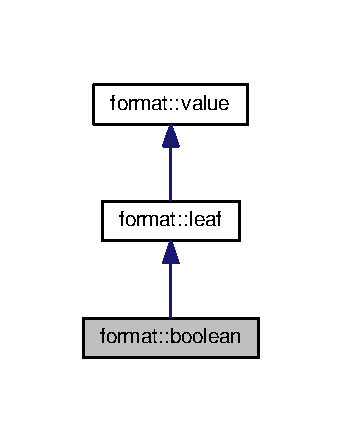
\includegraphics[width=164pt]{classformat_1_1boolean__inherit__graph}
\end{center}
\end{figure}


Collaboration diagram for format\+:\+:boolean\+:
\nopagebreak
\begin{figure}[H]
\begin{center}
\leavevmode
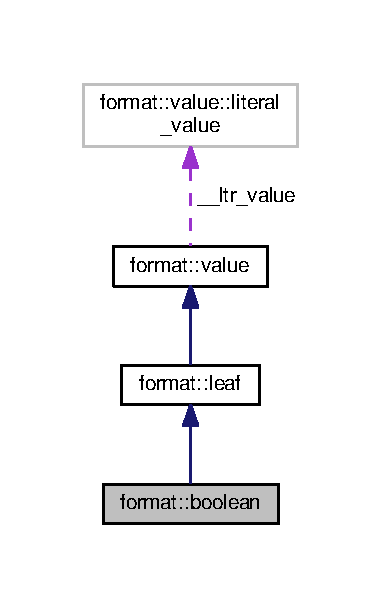
\includegraphics[width=183pt]{classformat_1_1boolean__coll__graph}
\end{center}
\end{figure}
\subsection*{Public Member Functions}
\begin{DoxyCompactItemize}
\item 
\hyperlink{classformat_1_1boolean_a7dd40c3ccee50e87df9bfadfe450ea14}{boolean} ()\hypertarget{classformat_1_1boolean_a7dd40c3ccee50e87df9bfadfe450ea14}{}\label{classformat_1_1boolean_a7dd40c3ccee50e87df9bfadfe450ea14}

\begin{DoxyCompactList}\small\item\em Boolean. \end{DoxyCompactList}\item 
\hyperlink{classformat_1_1boolean_a11ab54785dc8b08f9920b9bb9de0a346}{boolean} (const bool \hyperlink{classformat_1_1value_aa6b85823936bf7b8ab78d3f8d443c00d}{value})
\begin{DoxyCompactList}\small\item\em Boolean. \end{DoxyCompactList}\item 
\hyperlink{classformat_1_1boolean_aa1d20e80f24d862624e55dd4c5a99844}{boolean} (const \hyperlink{classformat_1_1boolean}{boolean} \&other)=default
\begin{DoxyCompactList}\small\item\em Boolean. \end{DoxyCompactList}\item 
virtual \hyperlink{classformat_1_1boolean_abbfeccbfc4d740e4cfc3667d324fbbc7}{$\sim$boolean} () override=default\hypertarget{classformat_1_1boolean_abbfeccbfc4d740e4cfc3667d324fbbc7}{}\label{classformat_1_1boolean_abbfeccbfc4d740e4cfc3667d324fbbc7}

\begin{DoxyCompactList}\small\item\em $\sim$\+Boolean \end{DoxyCompactList}\item 
virtual \hyperlink{classformat_1_1value_aa6b85823936bf7b8ab78d3f8d443c00d}{value} $\ast$ \hyperlink{classformat_1_1boolean_aed9485ecc21695be4ef8f03cd1034b1e}{clone} () const override
\begin{DoxyCompactList}\small\item\em clone \end{DoxyCompactList}\item 
virtual size\+\_\+t \hyperlink{classformat_1_1boolean_a3524e3f55c14f667563774b51aa3ffa5}{str\+\_\+length} () const noexceptoverride
\begin{DoxyCompactList}\small\item\em str\+Length \end{DoxyCompactList}\item 
virtual \hyperlink{classformat_1_1value_aa0334be06389a7b14af485fa0cd3aa21}{value\+\_\+t} \hyperlink{classformat_1_1boolean_a91dccd7986764af76b70627a348f27a4}{type} () const noexceptoverride
\begin{DoxyCompactList}\small\item\em type \end{DoxyCompactList}\item 
\hyperlink{classformat_1_1value_aa6b85823936bf7b8ab78d3f8d443c00d}{value} \& \hyperlink{classformat_1_1boolean_acc67b6aa9c4caec2f888d27f32116345}{operator=} (\hyperlink{classformat_1_1boolean}{boolean} \&b)
\begin{DoxyCompactList}\small\item\em operator = \end{DoxyCompactList}\item 
\hyperlink{classformat_1_1value_aa6b85823936bf7b8ab78d3f8d443c00d}{value} \& \hyperlink{classformat_1_1boolean_a430369f7677663e5c61a77ac01e4383f}{\+\_\+assign} (const \hyperlink{classformat_1_1boolean}{boolean} \&nv)
\begin{DoxyCompactList}\small\item\em assign \end{DoxyCompactList}\item 
bool \hyperlink{classformat_1_1boolean_a125e4f567867c95f1f36faee741bc817}{get} () const 
\begin{DoxyCompactList}\small\item\em value \end{DoxyCompactList}\end{DoxyCompactItemize}
\subsection*{Protected Member Functions}
\begin{DoxyCompactItemize}
\item 
\hyperlink{classformat_1_1boolean_a7613c19f7e09d9bc1abd67003883e3a7}{boolean} (\hyperlink{classformat_1_1json}{json} $\ast$\hyperlink{classformat_1_1value_a86c03ec8810bfd0d60ec49095120040d}{parent}, const bool \hyperlink{classformat_1_1value_aa6b85823936bf7b8ab78d3f8d443c00d}{value})
\begin{DoxyCompactList}\small\item\em boolean \end{DoxyCompactList}\item 
virtual const wchar\+\_\+t $\ast$ \hyperlink{classformat_1_1boolean_a6c3d3fc4e0a046f2070c5513ce61b12b}{\+\_\+parse} (const wchar\+\_\+t $\ast$\hyperlink{classformat_1_1json}{json}) override
\begin{DoxyCompactList}\small\item\em parse \end{DoxyCompactList}\item 
virtual void \hyperlink{classformat_1_1boolean_ab72d7e3749eaaaa8367150f816792ae2}{\+\_\+clear} ()\hypertarget{classformat_1_1boolean_ab72d7e3749eaaaa8367150f816792ae2}{}\label{classformat_1_1boolean_ab72d7e3749eaaaa8367150f816792ae2}

\begin{DoxyCompactList}\small\item\em \+\_\+clear \end{DoxyCompactList}\item 
virtual \hyperlink{classformat_1_1value_aa6b85823936bf7b8ab78d3f8d443c00d}{value} $\ast$ \hyperlink{classformat_1_1boolean_aa736f994233dad5fa8fcef030e50e2d7}{\+\_\+clone} (const \hyperlink{classformat_1_1value_aa6b85823936bf7b8ab78d3f8d443c00d}{value} \&other) override
\begin{DoxyCompactList}\small\item\em \+\_\+clone \end{DoxyCompactList}\item 
virtual const wchar\+\_\+t $\ast$ \hyperlink{classformat_1_1boolean_a8ca18cfd6036fe8d0255b08c91eb3e30}{\+\_\+to\+\_\+string} (wchar\+\_\+t $\ast$=0) const override
\begin{DoxyCompactList}\small\item\em str\+Value \end{DoxyCompactList}\end{DoxyCompactItemize}
\subsection*{Protected Attributes}
\begin{DoxyCompactItemize}
\item 
bool \hyperlink{classformat_1_1boolean_a7216c07536040efd3c486ef232008af4}{\+\_\+boolean\+\_\+value}\hypertarget{classformat_1_1boolean_a7216c07536040efd3c486ef232008af4}{}\label{classformat_1_1boolean_a7216c07536040efd3c486ef232008af4}

\begin{DoxyCompactList}\small\item\em \+\_\+boolean\+\_\+value \end{DoxyCompactList}\end{DoxyCompactItemize}
\subsection*{Friends}
\begin{DoxyCompactItemize}
\item 
\hyperlink{classformat_1_1boolean}{boolean} $\ast$ {\bfseries \+\_\+\+\_\+call\+\_\+boolean} (\hyperlink{classformat_1_1json}{json} $\ast$\hyperlink{classformat_1_1value_a86c03ec8810bfd0d60ec49095120040d}{parent}, bool b)\hypertarget{classformat_1_1boolean_a676e355d222bbbb0311f47dc983faf60}{}\label{classformat_1_1boolean_a676e355d222bbbb0311f47dc983faf60}

\end{DoxyCompactItemize}
\subsection*{Additional Inherited Members}


\subsection{Detailed Description}
The boolean class. 

\subsection{Constructor \& Destructor Documentation}
\index{format\+::boolean@{format\+::boolean}!boolean@{boolean}}
\index{boolean@{boolean}!format\+::boolean@{format\+::boolean}}
\subsubsection[{\texorpdfstring{boolean(const bool value)}{boolean(const bool value)}}]{\setlength{\rightskip}{0pt plus 5cm}format\+::boolean\+::boolean (
\begin{DoxyParamCaption}
\item[{const bool}]{value}
\end{DoxyParamCaption}
)\hspace{0.3cm}{\ttfamily [inline]}}\hypertarget{classformat_1_1boolean_a11ab54785dc8b08f9920b9bb9de0a346}{}\label{classformat_1_1boolean_a11ab54785dc8b08f9920b9bb9de0a346}


Boolean. 


\begin{DoxyParams}{Parameters}
{\em value} & \\
\hline
\end{DoxyParams}
\index{format\+::boolean@{format\+::boolean}!boolean@{boolean}}
\index{boolean@{boolean}!format\+::boolean@{format\+::boolean}}
\subsubsection[{\texorpdfstring{boolean(const boolean \&other)=default}{boolean(const boolean &other)=default}}]{\setlength{\rightskip}{0pt plus 5cm}format\+::boolean\+::boolean (
\begin{DoxyParamCaption}
\item[{const {\bf boolean} \&}]{other}
\end{DoxyParamCaption}
)\hspace{0.3cm}{\ttfamily [default]}}\hypertarget{classformat_1_1boolean_aa1d20e80f24d862624e55dd4c5a99844}{}\label{classformat_1_1boolean_aa1d20e80f24d862624e55dd4c5a99844}


Boolean. 


\begin{DoxyParams}{Parameters}
{\em other} & \\
\hline
\end{DoxyParams}
\index{format\+::boolean@{format\+::boolean}!boolean@{boolean}}
\index{boolean@{boolean}!format\+::boolean@{format\+::boolean}}
\subsubsection[{\texorpdfstring{boolean(json $\ast$parent, const bool value)}{boolean(json *parent, const bool value)}}]{\setlength{\rightskip}{0pt plus 5cm}format\+::boolean\+::boolean (
\begin{DoxyParamCaption}
\item[{{\bf json} $\ast$}]{parent, }
\item[{const bool}]{value}
\end{DoxyParamCaption}
)\hspace{0.3cm}{\ttfamily [inline]}, {\ttfamily [protected]}}\hypertarget{classformat_1_1boolean_a7613c19f7e09d9bc1abd67003883e3a7}{}\label{classformat_1_1boolean_a7613c19f7e09d9bc1abd67003883e3a7}


boolean 


\begin{DoxyParams}{Parameters}
{\em parent} & \\
\hline
{\em value} & \\
\hline
\end{DoxyParams}


\subsection{Member Function Documentation}
\index{format\+::boolean@{format\+::boolean}!\+\_\+assign@{\+\_\+assign}}
\index{\+\_\+assign@{\+\_\+assign}!format\+::boolean@{format\+::boolean}}
\subsubsection[{\texorpdfstring{\+\_\+assign(const boolean \&nv)}{_assign(const boolean &nv)}}]{\setlength{\rightskip}{0pt plus 5cm}{\bf value}\& format\+::boolean\+::\+\_\+assign (
\begin{DoxyParamCaption}
\item[{const {\bf boolean} \&}]{nv}
\end{DoxyParamCaption}
)\hspace{0.3cm}{\ttfamily [inline]}}\hypertarget{classformat_1_1boolean_a430369f7677663e5c61a77ac01e4383f}{}\label{classformat_1_1boolean_a430369f7677663e5c61a77ac01e4383f}


assign 


\begin{DoxyParams}{Parameters}
{\em nv} & \\
\hline
\end{DoxyParams}
\begin{DoxyReturn}{Returns}

\end{DoxyReturn}
\index{format\+::boolean@{format\+::boolean}!\+\_\+clone@{\+\_\+clone}}
\index{\+\_\+clone@{\+\_\+clone}!format\+::boolean@{format\+::boolean}}
\subsubsection[{\texorpdfstring{\+\_\+clone(const value \&other) override}{_clone(const value &other) override}}]{\setlength{\rightskip}{0pt plus 5cm}virtual {\bf value}$\ast$ format\+::boolean\+::\+\_\+clone (
\begin{DoxyParamCaption}
\item[{const {\bf value} \&}]{other}
\end{DoxyParamCaption}
)\hspace{0.3cm}{\ttfamily [inline]}, {\ttfamily [override]}, {\ttfamily [protected]}, {\ttfamily [virtual]}}\hypertarget{classformat_1_1boolean_aa736f994233dad5fa8fcef030e50e2d7}{}\label{classformat_1_1boolean_aa736f994233dad5fa8fcef030e50e2d7}


\+\_\+clone 

\begin{DoxyReturn}{Returns}

\end{DoxyReturn}


Implements \hyperlink{classformat_1_1leaf_a45f6e4e09027122e445ba3b8352aec14}{format\+::leaf}.

\index{format\+::boolean@{format\+::boolean}!\+\_\+parse@{\+\_\+parse}}
\index{\+\_\+parse@{\+\_\+parse}!format\+::boolean@{format\+::boolean}}
\subsubsection[{\texorpdfstring{\+\_\+parse(const wchar\+\_\+t $\ast$json) override}{_parse(const wchar_t *json) override}}]{\setlength{\rightskip}{0pt plus 5cm}virtual const wchar\+\_\+t$\ast$ format\+::boolean\+::\+\_\+parse (
\begin{DoxyParamCaption}
\item[{const wchar\+\_\+t $\ast$}]{json}
\end{DoxyParamCaption}
)\hspace{0.3cm}{\ttfamily [inline]}, {\ttfamily [override]}, {\ttfamily [protected]}, {\ttfamily [virtual]}}\hypertarget{classformat_1_1boolean_a6c3d3fc4e0a046f2070c5513ce61b12b}{}\label{classformat_1_1boolean_a6c3d3fc4e0a046f2070c5513ce61b12b}


parse 


\begin{DoxyParams}{Parameters}
{\em json} & \\
\hline
\end{DoxyParams}
\begin{DoxyReturn}{Returns}

\end{DoxyReturn}


Implements \hyperlink{classformat_1_1value_a7859b1aa48f667a83e091f0eba22d4a1}{format\+::value}.

\index{format\+::boolean@{format\+::boolean}!\+\_\+to\+\_\+string@{\+\_\+to\+\_\+string}}
\index{\+\_\+to\+\_\+string@{\+\_\+to\+\_\+string}!format\+::boolean@{format\+::boolean}}
\subsubsection[{\texorpdfstring{\+\_\+to\+\_\+string(wchar\+\_\+t $\ast$=0) const override}{_to_string(wchar_t *=0) const override}}]{\setlength{\rightskip}{0pt plus 5cm}virtual const wchar\+\_\+t$\ast$ format\+::boolean\+::\+\_\+to\+\_\+string (
\begin{DoxyParamCaption}
\item[{wchar\+\_\+t $\ast$}]{ = {\ttfamily 0}}
\end{DoxyParamCaption}
) const\hspace{0.3cm}{\ttfamily [inline]}, {\ttfamily [override]}, {\ttfamily [protected]}, {\ttfamily [virtual]}}\hypertarget{classformat_1_1boolean_a8ca18cfd6036fe8d0255b08c91eb3e30}{}\label{classformat_1_1boolean_a8ca18cfd6036fe8d0255b08c91eb3e30}


str\+Value 

\begin{DoxyReturn}{Returns}

\end{DoxyReturn}


Implements \hyperlink{classformat_1_1value_a94ed31f07b19866495297472accd33a8}{format\+::value}.

\index{format\+::boolean@{format\+::boolean}!clone@{clone}}
\index{clone@{clone}!format\+::boolean@{format\+::boolean}}
\subsubsection[{\texorpdfstring{clone() const override}{clone() const override}}]{\setlength{\rightskip}{0pt plus 5cm}virtual {\bf value}$\ast$ format\+::boolean\+::clone (
\begin{DoxyParamCaption}
{}
\end{DoxyParamCaption}
) const\hspace{0.3cm}{\ttfamily [inline]}, {\ttfamily [override]}, {\ttfamily [virtual]}}\hypertarget{classformat_1_1boolean_aed9485ecc21695be4ef8f03cd1034b1e}{}\label{classformat_1_1boolean_aed9485ecc21695be4ef8f03cd1034b1e}


clone 


\begin{DoxyParams}{Parameters}
{\em other} & \\
\hline
\end{DoxyParams}
\begin{DoxyReturn}{Returns}

\end{DoxyReturn}


Implements \hyperlink{classformat_1_1leaf_a861972c1866ab17d00e4b950d33d4ced}{format\+::leaf}.

\index{format\+::boolean@{format\+::boolean}!get@{get}}
\index{get@{get}!format\+::boolean@{format\+::boolean}}
\subsubsection[{\texorpdfstring{get() const }{get() const }}]{\setlength{\rightskip}{0pt plus 5cm}bool format\+::boolean\+::get (
\begin{DoxyParamCaption}
{}
\end{DoxyParamCaption}
) const\hspace{0.3cm}{\ttfamily [inline]}}\hypertarget{classformat_1_1boolean_a125e4f567867c95f1f36faee741bc817}{}\label{classformat_1_1boolean_a125e4f567867c95f1f36faee741bc817}


value 

\begin{DoxyReturn}{Returns}

\end{DoxyReturn}
\index{format\+::boolean@{format\+::boolean}!operator=@{operator=}}
\index{operator=@{operator=}!format\+::boolean@{format\+::boolean}}
\subsubsection[{\texorpdfstring{operator=(boolean \&b)}{operator=(boolean &b)}}]{\setlength{\rightskip}{0pt plus 5cm}{\bf value}\& format\+::boolean\+::operator= (
\begin{DoxyParamCaption}
\item[{{\bf boolean} \&}]{b}
\end{DoxyParamCaption}
)\hspace{0.3cm}{\ttfamily [inline]}}\hypertarget{classformat_1_1boolean_acc67b6aa9c4caec2f888d27f32116345}{}\label{classformat_1_1boolean_acc67b6aa9c4caec2f888d27f32116345}


operator = 


\begin{DoxyParams}{Parameters}
{\em b} & \\
\hline
\end{DoxyParams}
\begin{DoxyReturn}{Returns}

\end{DoxyReturn}
\index{format\+::boolean@{format\+::boolean}!str\+\_\+length@{str\+\_\+length}}
\index{str\+\_\+length@{str\+\_\+length}!format\+::boolean@{format\+::boolean}}
\subsubsection[{\texorpdfstring{str\+\_\+length() const noexceptoverride}{str_length() const noexceptoverride}}]{\setlength{\rightskip}{0pt plus 5cm}virtual size\+\_\+t format\+::boolean\+::str\+\_\+length (
\begin{DoxyParamCaption}
{}
\end{DoxyParamCaption}
) const\hspace{0.3cm}{\ttfamily [inline]}, {\ttfamily [override]}, {\ttfamily [virtual]}, {\ttfamily [noexcept]}}\hypertarget{classformat_1_1boolean_a3524e3f55c14f667563774b51aa3ffa5}{}\label{classformat_1_1boolean_a3524e3f55c14f667563774b51aa3ffa5}


str\+Length 

\begin{DoxyReturn}{Returns}

\end{DoxyReturn}


Implements \hyperlink{classformat_1_1value_a399280e27e629db0582b5781b90ca58b}{format\+::value}.

\index{format\+::boolean@{format\+::boolean}!type@{type}}
\index{type@{type}!format\+::boolean@{format\+::boolean}}
\subsubsection[{\texorpdfstring{type() const noexceptoverride}{type() const noexceptoverride}}]{\setlength{\rightskip}{0pt plus 5cm}virtual {\bf value\+\_\+t} format\+::boolean\+::type (
\begin{DoxyParamCaption}
{}
\end{DoxyParamCaption}
) const\hspace{0.3cm}{\ttfamily [inline]}, {\ttfamily [override]}, {\ttfamily [virtual]}, {\ttfamily [noexcept]}}\hypertarget{classformat_1_1boolean_a91dccd7986764af76b70627a348f27a4}{}\label{classformat_1_1boolean_a91dccd7986764af76b70627a348f27a4}


type 

\begin{DoxyReturn}{Returns}

\end{DoxyReturn}


Implements \hyperlink{classformat_1_1leaf_ac29de88719f2da4d262255ef8a234ced}{format\+::leaf}.



The documentation for this class was generated from the following file\+:\begin{DoxyCompactItemize}
\item 
json\+\_\+boolean.\+h\end{DoxyCompactItemize}

\hypertarget{structformat}{}\section{format Struct Reference}
\label{structformat}\index{format@{format}}


Inheritance diagram for format\+:
\nopagebreak
\begin{figure}[H]
\begin{center}
\leavevmode
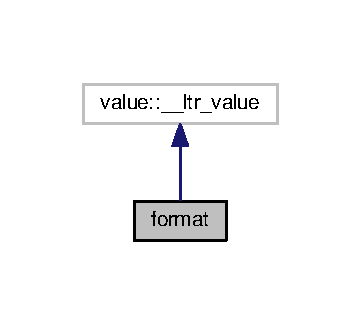
\includegraphics[width=173pt]{structformat__inherit__graph}
\end{center}
\end{figure}


Collaboration diagram for format\+:
\nopagebreak
\begin{figure}[H]
\begin{center}
\leavevmode
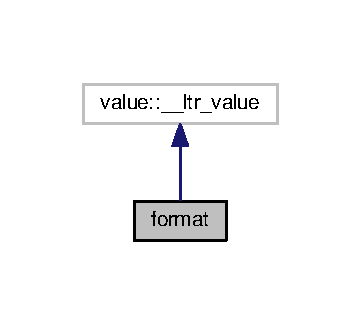
\includegraphics[width=173pt]{structformat__coll__graph}
\end{center}
\end{figure}
\subsection*{Classes}
\begin{DoxyCompactItemize}
\item 
class \hyperlink{classformat_1_1value}{value}
\end{DoxyCompactItemize}
\subsection*{Public Types}
\begin{DoxyCompactItemize}
\item 
typedef value $\ast$($\ast$ {\bfseries reviver}) (const wchar\+\_\+t $\ast$, value $\ast$)\hypertarget{structformat_a8b8bca9d689121d31347a4d47f79e61f}{}\label{structformat_a8b8bca9d689121d31347a4d47f79e61f}

\end{DoxyCompactItemize}


The documentation for this struct was generated from the following files\+:\begin{DoxyCompactItemize}
\item 
json\+\_\+value.\+cpp\item 
json\+\_\+json.\+h\end{DoxyCompactItemize}

\hypertarget{classformat_1_1array_1_1iterator}{}\section{format\+:\+:array\+:\+:iterator Class Reference}
\label{classformat_1_1array_1_1iterator}\index{format\+::array\+::iterator@{format\+::array\+::iterator}}


The iterator class.  




{\ttfamily \#include $<$json\+\_\+array.\+h$>$}



Inheritance diagram for format\+:\+:array\+:\+:iterator\+:
\nopagebreak
\begin{figure}[H]
\begin{center}
\leavevmode
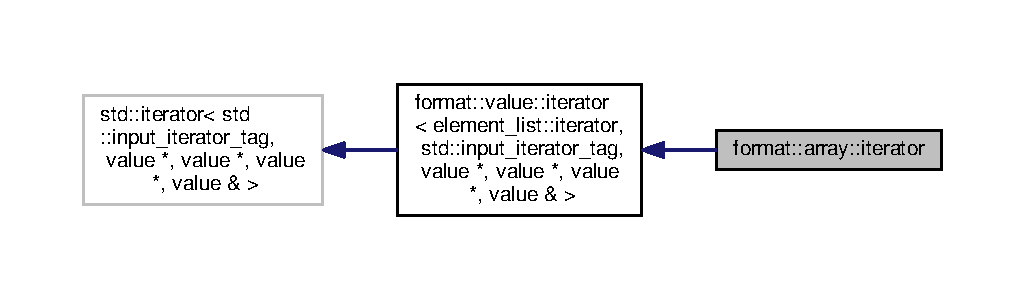
\includegraphics[width=350pt]{classformat_1_1array_1_1iterator__inherit__graph}
\end{center}
\end{figure}


Collaboration diagram for format\+:\+:array\+:\+:iterator\+:
\nopagebreak
\begin{figure}[H]
\begin{center}
\leavevmode
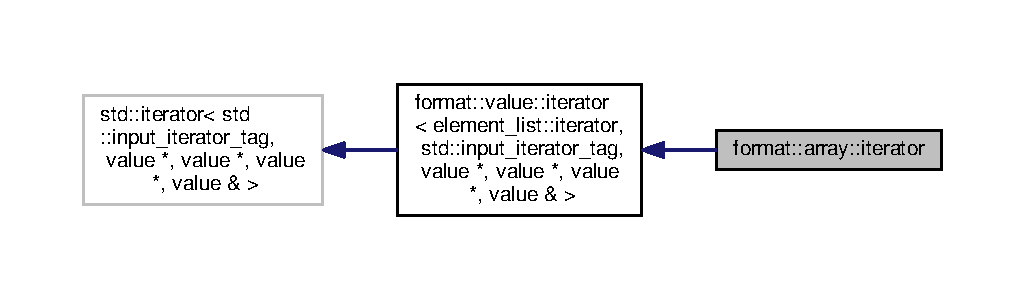
\includegraphics[width=350pt]{classformat_1_1array_1_1iterator__coll__graph}
\end{center}
\end{figure}
\subsection*{Public Member Functions}
\begin{DoxyCompactItemize}
\item 
\hyperlink{classformat_1_1array_1_1iterator_abdf89f18e19ceaba55b348b50d4a0e61}{iterator} ()\hypertarget{classformat_1_1array_1_1iterator_abdf89f18e19ceaba55b348b50d4a0e61}{}\label{classformat_1_1array_1_1iterator_abdf89f18e19ceaba55b348b50d4a0e61}

\begin{DoxyCompactList}\small\item\em iterator \end{DoxyCompactList}\item 
\hyperlink{classformat_1_1array_1_1iterator_ac60fbed78ee29e41c017d75473ae0c2d}{iterator} (element\+\_\+list\+::iterator it)
\begin{DoxyCompactList}\small\item\em iterator \end{DoxyCompactList}\item 
\hyperlink{classformat_1_1array_1_1iterator_a940bc2cf6d3854281d8949eb879bd50a}{iterator} (const \hyperlink{classformat_1_1array_1_1iterator}{iterator} \&other)
\begin{DoxyCompactList}\small\item\em iterator \end{DoxyCompactList}\item 
virtual \hyperlink{classformat_1_1array_1_1iterator_aa8af0e6585ea44ed71f742ab2590da14}{$\sim$iterator} ()=default\hypertarget{classformat_1_1array_1_1iterator_aa8af0e6585ea44ed71f742ab2590da14}{}\label{classformat_1_1array_1_1iterator_aa8af0e6585ea44ed71f742ab2590da14}

\begin{DoxyCompactList}\small\item\em $\sim$\+Iterator \end{DoxyCompactList}\item 
reference \hyperlink{classformat_1_1array_1_1iterator_a3a5e953a8dcea660e44a324251e9a6bb}{operator$\ast$} ()
\begin{DoxyCompactList}\small\item\em operator $\ast$ \end{DoxyCompactList}\end{DoxyCompactItemize}
\subsection*{Additional Inherited Members}


\subsection{Detailed Description}
The iterator class. 

\subsection{Constructor \& Destructor Documentation}
\index{format\+::array\+::iterator@{format\+::array\+::iterator}!iterator@{iterator}}
\index{iterator@{iterator}!format\+::array\+::iterator@{format\+::array\+::iterator}}
\subsubsection[{\texorpdfstring{iterator(element\+\_\+list\+::iterator it)}{iterator(element_list::iterator it)}}]{\setlength{\rightskip}{0pt plus 5cm}format\+::array\+::iterator\+::iterator (
\begin{DoxyParamCaption}
\item[{element\+\_\+list\+::iterator}]{it}
\end{DoxyParamCaption}
)\hspace{0.3cm}{\ttfamily [inline]}}\hypertarget{classformat_1_1array_1_1iterator_ac60fbed78ee29e41c017d75473ae0c2d}{}\label{classformat_1_1array_1_1iterator_ac60fbed78ee29e41c017d75473ae0c2d}


iterator 


\begin{DoxyParams}{Parameters}
{\em it} & \\
\hline
\end{DoxyParams}
\index{format\+::array\+::iterator@{format\+::array\+::iterator}!iterator@{iterator}}
\index{iterator@{iterator}!format\+::array\+::iterator@{format\+::array\+::iterator}}
\subsubsection[{\texorpdfstring{iterator(const iterator \&other)}{iterator(const iterator &other)}}]{\setlength{\rightskip}{0pt plus 5cm}format\+::array\+::iterator\+::iterator (
\begin{DoxyParamCaption}
\item[{const {\bf iterator} \&}]{other}
\end{DoxyParamCaption}
)\hspace{0.3cm}{\ttfamily [inline]}}\hypertarget{classformat_1_1array_1_1iterator_a940bc2cf6d3854281d8949eb879bd50a}{}\label{classformat_1_1array_1_1iterator_a940bc2cf6d3854281d8949eb879bd50a}


iterator 


\begin{DoxyParams}{Parameters}
{\em other} & \\
\hline
\end{DoxyParams}


\subsection{Member Function Documentation}
\index{format\+::array\+::iterator@{format\+::array\+::iterator}!operator$\ast$@{operator$\ast$}}
\index{operator$\ast$@{operator$\ast$}!format\+::array\+::iterator@{format\+::array\+::iterator}}
\subsubsection[{\texorpdfstring{operator$\ast$()}{operator*()}}]{\setlength{\rightskip}{0pt plus 5cm}reference format\+::array\+::iterator\+::operator$\ast$ (
\begin{DoxyParamCaption}
{}
\end{DoxyParamCaption}
)\hspace{0.3cm}{\ttfamily [inline]}}\hypertarget{classformat_1_1array_1_1iterator_a3a5e953a8dcea660e44a324251e9a6bb}{}\label{classformat_1_1array_1_1iterator_a3a5e953a8dcea660e44a324251e9a6bb}


operator $\ast$ 

\begin{DoxyReturn}{Returns}

\end{DoxyReturn}


The documentation for this class was generated from the following file\+:\begin{DoxyCompactItemize}
\item 
json\+\_\+array.\+h\end{DoxyCompactItemize}

\hypertarget{classformat_1_1leaf_1_1iterator}{}\section{format\+:\+:leaf\+:\+:iterator Class Reference}
\label{classformat_1_1leaf_1_1iterator}\index{format\+::leaf\+::iterator@{format\+::leaf\+::iterator}}


The iterator class.  




{\ttfamily \#include $<$json\+\_\+leaf.\+h$>$}



Inheritance diagram for format\+:\+:leaf\+:\+:iterator\+:
\nopagebreak
\begin{figure}[H]
\begin{center}
\leavevmode
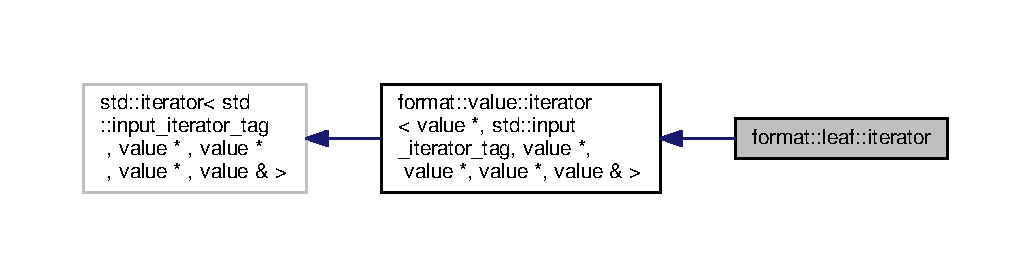
\includegraphics[width=350pt]{classformat_1_1leaf_1_1iterator__inherit__graph}
\end{center}
\end{figure}


Collaboration diagram for format\+:\+:leaf\+:\+:iterator\+:
\nopagebreak
\begin{figure}[H]
\begin{center}
\leavevmode
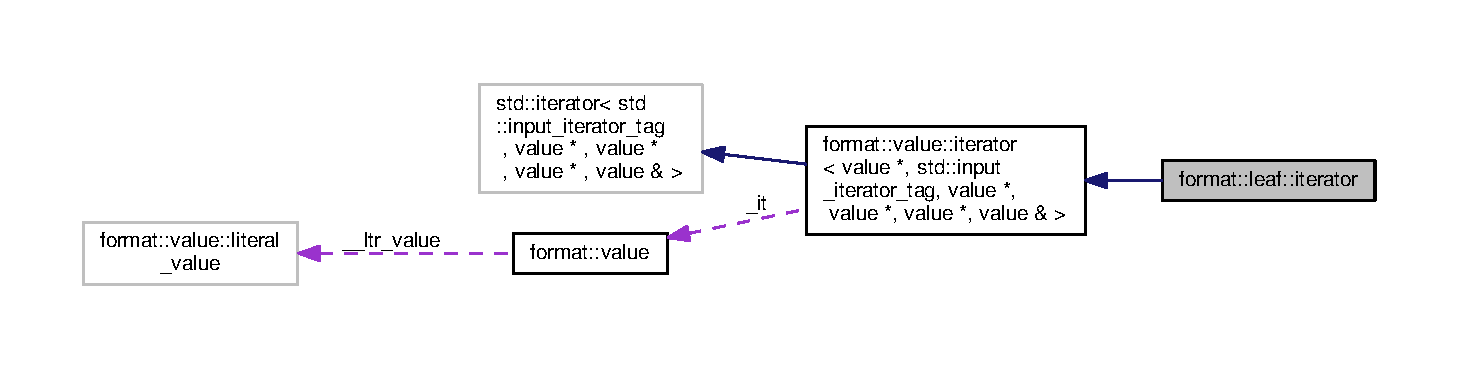
\includegraphics[width=350pt]{classformat_1_1leaf_1_1iterator__coll__graph}
\end{center}
\end{figure}
\subsection*{Public Member Functions}
\begin{DoxyCompactItemize}
\item 
\hyperlink{classformat_1_1leaf_1_1iterator_a94f19614cd58bf64bd15b465780b3007}{iterator} (\hyperlink{classformat_1_1leaf}{leaf} $\ast$\hyperlink{classformat_1_1value_aa6b85823936bf7b8ab78d3f8d443c00d}{value}=0)
\begin{DoxyCompactList}\small\item\em iterator \end{DoxyCompactList}\item 
\hyperlink{classformat_1_1leaf_1_1iterator_aa5942a9e1620a8009fe139e3affaf19f}{iterator} (const \hyperlink{classformat_1_1leaf_1_1iterator}{iterator} \&other)=default
\begin{DoxyCompactList}\small\item\em iterator \end{DoxyCompactList}\item 
\hyperlink{classformat_1_1leaf_1_1iterator_ae22dd7c3629ba7cc5fac7c2b7234d565}{$\sim$iterator} ()=default\hypertarget{classformat_1_1leaf_1_1iterator_ae22dd7c3629ba7cc5fac7c2b7234d565}{}\label{classformat_1_1leaf_1_1iterator_ae22dd7c3629ba7cc5fac7c2b7234d565}

\begin{DoxyCompactList}\small\item\em $\sim$iterator \end{DoxyCompactList}\item 
reference \hyperlink{classformat_1_1leaf_1_1iterator_ac605a437a33d536d4ec68bdf3de32dc8}{operator$\ast$} ()
\begin{DoxyCompactList}\small\item\em operator $\ast$ \end{DoxyCompactList}\end{DoxyCompactItemize}
\subsection*{Additional Inherited Members}


\subsection{Detailed Description}
The iterator class. 

\subsection{Constructor \& Destructor Documentation}
\index{format\+::leaf\+::iterator@{format\+::leaf\+::iterator}!iterator@{iterator}}
\index{iterator@{iterator}!format\+::leaf\+::iterator@{format\+::leaf\+::iterator}}
\subsubsection[{\texorpdfstring{iterator(leaf $\ast$value=0)}{iterator(leaf *value=0)}}]{\setlength{\rightskip}{0pt plus 5cm}format\+::leaf\+::iterator\+::iterator (
\begin{DoxyParamCaption}
\item[{{\bf leaf} $\ast$}]{value = {\ttfamily 0}}
\end{DoxyParamCaption}
)\hspace{0.3cm}{\ttfamily [inline]}}\hypertarget{classformat_1_1leaf_1_1iterator_a94f19614cd58bf64bd15b465780b3007}{}\label{classformat_1_1leaf_1_1iterator_a94f19614cd58bf64bd15b465780b3007}


iterator 


\begin{DoxyParams}{Parameters}
{\em value} & \\
\hline
\end{DoxyParams}
\index{format\+::leaf\+::iterator@{format\+::leaf\+::iterator}!iterator@{iterator}}
\index{iterator@{iterator}!format\+::leaf\+::iterator@{format\+::leaf\+::iterator}}
\subsubsection[{\texorpdfstring{iterator(const iterator \&other)=default}{iterator(const iterator &other)=default}}]{\setlength{\rightskip}{0pt plus 5cm}format\+::leaf\+::iterator\+::iterator (
\begin{DoxyParamCaption}
\item[{const {\bf iterator} \&}]{other}
\end{DoxyParamCaption}
)\hspace{0.3cm}{\ttfamily [default]}}\hypertarget{classformat_1_1leaf_1_1iterator_aa5942a9e1620a8009fe139e3affaf19f}{}\label{classformat_1_1leaf_1_1iterator_aa5942a9e1620a8009fe139e3affaf19f}


iterator 


\begin{DoxyParams}{Parameters}
{\em other} & \\
\hline
\end{DoxyParams}


\subsection{Member Function Documentation}
\index{format\+::leaf\+::iterator@{format\+::leaf\+::iterator}!operator$\ast$@{operator$\ast$}}
\index{operator$\ast$@{operator$\ast$}!format\+::leaf\+::iterator@{format\+::leaf\+::iterator}}
\subsubsection[{\texorpdfstring{operator$\ast$()}{operator*()}}]{\setlength{\rightskip}{0pt plus 5cm}reference format\+::leaf\+::iterator\+::operator$\ast$ (
\begin{DoxyParamCaption}
{}
\end{DoxyParamCaption}
)\hspace{0.3cm}{\ttfamily [inline]}}\hypertarget{classformat_1_1leaf_1_1iterator_ac605a437a33d536d4ec68bdf3de32dc8}{}\label{classformat_1_1leaf_1_1iterator_ac605a437a33d536d4ec68bdf3de32dc8}


operator $\ast$ 

\begin{DoxyReturn}{Returns}

\end{DoxyReturn}


The documentation for this class was generated from the following file\+:\begin{DoxyCompactItemize}
\item 
json\+\_\+leaf.\+h\end{DoxyCompactItemize}

\hypertarget{classformat_1_1value_1_1iterator}{}\section{format\+:\+:value\+:\+:iterator$<$ Iterator, Category, T, Distance, Pointer, Reference $>$ Class Template Reference}
\label{classformat_1_1value_1_1iterator}\index{format\+::value\+::iterator$<$ Iterator, Category, T, Distance, Pointer, Reference $>$@{format\+::value\+::iterator$<$ Iterator, Category, T, Distance, Pointer, Reference $>$}}


The iterator class.  




{\ttfamily \#include $<$json\+\_\+value.\+h$>$}



Inheritance diagram for format\+:\+:value\+:\+:iterator$<$ Iterator, Category, T, Distance, Pointer, Reference $>$\+:
\nopagebreak
\begin{figure}[H]
\begin{center}
\leavevmode
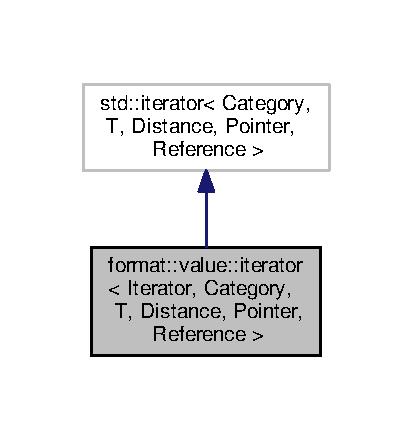
\includegraphics[width=198pt]{classformat_1_1value_1_1iterator__inherit__graph}
\end{center}
\end{figure}


Collaboration diagram for format\+:\+:value\+:\+:iterator$<$ Iterator, Category, T, Distance, Pointer, Reference $>$\+:
\nopagebreak
\begin{figure}[H]
\begin{center}
\leavevmode
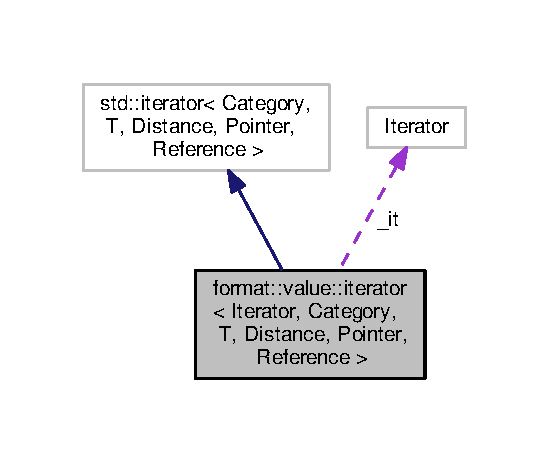
\includegraphics[width=264pt]{classformat_1_1value_1_1iterator__coll__graph}
\end{center}
\end{figure}
\subsection*{Public Member Functions}
\begin{DoxyCompactItemize}
\item 
\hyperlink{classformat_1_1value_1_1iterator_af16610a1645c2e393a1bbd49f8bc2ec9}{iterator} ()\hypertarget{classformat_1_1value_1_1iterator_af16610a1645c2e393a1bbd49f8bc2ec9}{}\label{classformat_1_1value_1_1iterator_af16610a1645c2e393a1bbd49f8bc2ec9}

\begin{DoxyCompactList}\small\item\em iterator \end{DoxyCompactList}\item 
\hyperlink{classformat_1_1value_1_1iterator_a859a232d4c628e3c9a4d52828f3dd545}{iterator} (Iterator it)\hypertarget{classformat_1_1value_1_1iterator_a859a232d4c628e3c9a4d52828f3dd545}{}\label{classformat_1_1value_1_1iterator_a859a232d4c628e3c9a4d52828f3dd545}

\begin{DoxyCompactList}\small\item\em iterator \end{DoxyCompactList}\item 
\hyperlink{classformat_1_1value_1_1iterator_a77fcd6c18b944b672761468008630d22}{iterator} (const \hyperlink{classformat_1_1value_1_1iterator}{iterator} \&other)
\begin{DoxyCompactList}\small\item\em iterator \end{DoxyCompactList}\item 
virtual \hyperlink{classformat_1_1value_1_1iterator_a7be0b1d4266e27c28bfd376908b5611c}{$\sim$iterator} ()=default\hypertarget{classformat_1_1value_1_1iterator_a7be0b1d4266e27c28bfd376908b5611c}{}\label{classformat_1_1value_1_1iterator_a7be0b1d4266e27c28bfd376908b5611c}

\begin{DoxyCompactList}\small\item\em $\sim$iterator \end{DoxyCompactList}\item 
\hyperlink{classformat_1_1value_1_1iterator}{iterator} \& \hyperlink{classformat_1_1value_1_1iterator_acc2de73af4df5a286d946b3808b11f55}{operator++} ()
\begin{DoxyCompactList}\small\item\em operator ++ \end{DoxyCompactList}\item 
\hyperlink{classformat_1_1value_1_1iterator}{iterator} \hyperlink{classformat_1_1value_1_1iterator_a5808bd24b5f0a29f08a79e816ccf0be8}{operator++} (int)
\begin{DoxyCompactList}\small\item\em operator ++ \end{DoxyCompactList}\item 
bool \hyperlink{classformat_1_1value_1_1iterator_aff47683163af5878a754a35a6f342e35}{operator==} (const \hyperlink{classformat_1_1value_1_1iterator}{iterator} \&rhs)
\begin{DoxyCompactList}\small\item\em operator == \end{DoxyCompactList}\item 
bool \hyperlink{classformat_1_1value_1_1iterator_a661669d9b3c4af651df0520e8c580eab}{operator!=} (const \hyperlink{classformat_1_1value_1_1iterator}{iterator} \&rhs)
\begin{DoxyCompactList}\small\item\em operator != \end{DoxyCompactList}\end{DoxyCompactItemize}
\subsection*{Protected Attributes}
\begin{DoxyCompactItemize}
\item 
Iterator \hyperlink{classformat_1_1value_1_1iterator_a5111b2fefd001383ed6a026f04fb47b9}{\+\_\+it}\hypertarget{classformat_1_1value_1_1iterator_a5111b2fefd001383ed6a026f04fb47b9}{}\label{classformat_1_1value_1_1iterator_a5111b2fefd001383ed6a026f04fb47b9}

\begin{DoxyCompactList}\small\item\em \+\_\+it \end{DoxyCompactList}\end{DoxyCompactItemize}


\subsection{Detailed Description}
\subsubsection*{template$<$class Iterator, class Category, class T, class Distance = std\+::ptrdiff\+\_\+t, class Pointer = T$\ast$, class Reference = T\&$>$\\*
class format\+::value\+::iterator$<$ Iterator, Category, T, Distance, Pointer, Reference $>$}

The iterator class. 

\subsection{Constructor \& Destructor Documentation}
\index{format\+::value\+::iterator@{format\+::value\+::iterator}!iterator@{iterator}}
\index{iterator@{iterator}!format\+::value\+::iterator@{format\+::value\+::iterator}}
\subsubsection[{\texorpdfstring{iterator(const iterator \&other)}{iterator(const iterator &other)}}]{\setlength{\rightskip}{0pt plus 5cm}template$<$class Iterator, class Category, class T, class Distance = std\+::ptrdiff\+\_\+t, class Pointer = T$\ast$, class Reference = T\&$>$ {\bf format\+::value\+::iterator}$<$ Iterator, Category, T, Distance, Pointer, Reference $>$\+::{\bf iterator} (
\begin{DoxyParamCaption}
\item[{const {\bf iterator}$<$ Iterator, Category, T, Distance, Pointer, Reference $>$ \&}]{other}
\end{DoxyParamCaption}
)\hspace{0.3cm}{\ttfamily [inline]}}\hypertarget{classformat_1_1value_1_1iterator_a77fcd6c18b944b672761468008630d22}{}\label{classformat_1_1value_1_1iterator_a77fcd6c18b944b672761468008630d22}


iterator 


\begin{DoxyParams}{Parameters}
{\em other} & \\
\hline
\end{DoxyParams}


\subsection{Member Function Documentation}
\index{format\+::value\+::iterator@{format\+::value\+::iterator}!operator"!=@{operator"!=}}
\index{operator"!=@{operator"!=}!format\+::value\+::iterator@{format\+::value\+::iterator}}
\subsubsection[{\texorpdfstring{operator"!=(const iterator \&rhs)}{operator!=(const iterator &rhs)}}]{\setlength{\rightskip}{0pt plus 5cm}template$<$class Iterator, class Category, class T, class Distance = std\+::ptrdiff\+\_\+t, class Pointer = T$\ast$, class Reference = T\&$>$ bool {\bf format\+::value\+::iterator}$<$ Iterator, Category, T, Distance, Pointer, Reference $>$\+::operator!= (
\begin{DoxyParamCaption}
\item[{const {\bf iterator}$<$ Iterator, Category, T, Distance, Pointer, Reference $>$ \&}]{rhs}
\end{DoxyParamCaption}
)\hspace{0.3cm}{\ttfamily [inline]}}\hypertarget{classformat_1_1value_1_1iterator_a661669d9b3c4af651df0520e8c580eab}{}\label{classformat_1_1value_1_1iterator_a661669d9b3c4af651df0520e8c580eab}


operator != 


\begin{DoxyParams}{Parameters}
{\em rhs} & \\
\hline
\end{DoxyParams}
\begin{DoxyReturn}{Returns}

\end{DoxyReturn}
\index{format\+::value\+::iterator@{format\+::value\+::iterator}!operator++@{operator++}}
\index{operator++@{operator++}!format\+::value\+::iterator@{format\+::value\+::iterator}}
\subsubsection[{\texorpdfstring{operator++()}{operator++()}}]{\setlength{\rightskip}{0pt plus 5cm}template$<$class Iterator, class Category, class T, class Distance = std\+::ptrdiff\+\_\+t, class Pointer = T$\ast$, class Reference = T\&$>$ {\bf iterator}\& {\bf format\+::value\+::iterator}$<$ Iterator, Category, T, Distance, Pointer, Reference $>$\+::operator++ (
\begin{DoxyParamCaption}
{}
\end{DoxyParamCaption}
)\hspace{0.3cm}{\ttfamily [inline]}}\hypertarget{classformat_1_1value_1_1iterator_acc2de73af4df5a286d946b3808b11f55}{}\label{classformat_1_1value_1_1iterator_acc2de73af4df5a286d946b3808b11f55}


operator ++ 

\begin{DoxyReturn}{Returns}

\end{DoxyReturn}
\index{format\+::value\+::iterator@{format\+::value\+::iterator}!operator++@{operator++}}
\index{operator++@{operator++}!format\+::value\+::iterator@{format\+::value\+::iterator}}
\subsubsection[{\texorpdfstring{operator++(int)}{operator++(int)}}]{\setlength{\rightskip}{0pt plus 5cm}template$<$class Iterator, class Category, class T, class Distance = std\+::ptrdiff\+\_\+t, class Pointer = T$\ast$, class Reference = T\&$>$ {\bf iterator} {\bf format\+::value\+::iterator}$<$ Iterator, Category, T, Distance, Pointer, Reference $>$\+::operator++ (
\begin{DoxyParamCaption}
\item[{int}]{}
\end{DoxyParamCaption}
)\hspace{0.3cm}{\ttfamily [inline]}}\hypertarget{classformat_1_1value_1_1iterator_a5808bd24b5f0a29f08a79e816ccf0be8}{}\label{classformat_1_1value_1_1iterator_a5808bd24b5f0a29f08a79e816ccf0be8}


operator ++ 

\begin{DoxyReturn}{Returns}

\end{DoxyReturn}
\index{format\+::value\+::iterator@{format\+::value\+::iterator}!operator==@{operator==}}
\index{operator==@{operator==}!format\+::value\+::iterator@{format\+::value\+::iterator}}
\subsubsection[{\texorpdfstring{operator==(const iterator \&rhs)}{operator==(const iterator &rhs)}}]{\setlength{\rightskip}{0pt plus 5cm}template$<$class Iterator, class Category, class T, class Distance = std\+::ptrdiff\+\_\+t, class Pointer = T$\ast$, class Reference = T\&$>$ bool {\bf format\+::value\+::iterator}$<$ Iterator, Category, T, Distance, Pointer, Reference $>$\+::operator== (
\begin{DoxyParamCaption}
\item[{const {\bf iterator}$<$ Iterator, Category, T, Distance, Pointer, Reference $>$ \&}]{rhs}
\end{DoxyParamCaption}
)\hspace{0.3cm}{\ttfamily [inline]}}\hypertarget{classformat_1_1value_1_1iterator_aff47683163af5878a754a35a6f342e35}{}\label{classformat_1_1value_1_1iterator_aff47683163af5878a754a35a6f342e35}


operator == 


\begin{DoxyParams}{Parameters}
{\em rhs} & \\
\hline
\end{DoxyParams}
\begin{DoxyReturn}{Returns}

\end{DoxyReturn}


The documentation for this class was generated from the following file\+:\begin{DoxyCompactItemize}
\item 
json\+\_\+value.\+h\end{DoxyCompactItemize}

\hypertarget{classformat_1_1object_1_1iterator}{}\section{format\+:\+:object\+:\+:iterator Class Reference}
\label{classformat_1_1object_1_1iterator}\index{format\+::object\+::iterator@{format\+::object\+::iterator}}


The iterator class.  




{\ttfamily \#include $<$json\+\_\+object.\+h$>$}



Inheritance diagram for format\+:\+:object\+:\+:iterator\+:
\nopagebreak
\begin{figure}[H]
\begin{center}
\leavevmode
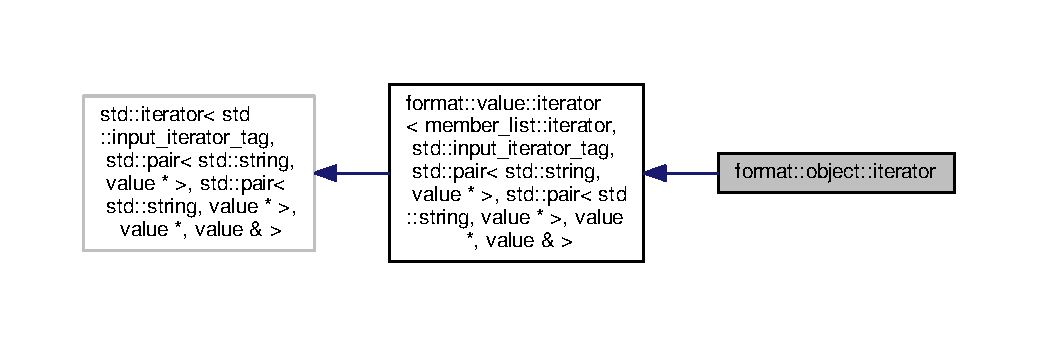
\includegraphics[width=350pt]{classformat_1_1object_1_1iterator__inherit__graph}
\end{center}
\end{figure}


Collaboration diagram for format\+:\+:object\+:\+:iterator\+:
\nopagebreak
\begin{figure}[H]
\begin{center}
\leavevmode
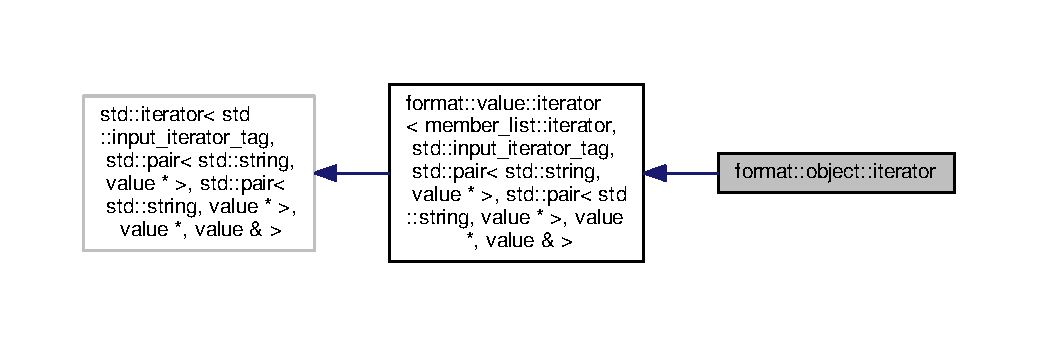
\includegraphics[width=350pt]{classformat_1_1object_1_1iterator__coll__graph}
\end{center}
\end{figure}
\subsection*{Public Member Functions}
\begin{DoxyCompactItemize}
\item 
\hyperlink{classformat_1_1object_1_1iterator_a53abe04a3141d1ef48bd569d0d33e2c9}{iterator} ()\hypertarget{classformat_1_1object_1_1iterator_a53abe04a3141d1ef48bd569d0d33e2c9}{}\label{classformat_1_1object_1_1iterator_a53abe04a3141d1ef48bd569d0d33e2c9}

\begin{DoxyCompactList}\small\item\em iterator \end{DoxyCompactList}\item 
\hyperlink{classformat_1_1object_1_1iterator_a5ca07e90b6e39203b092f8a944ed2e3d}{iterator} (member\+\_\+list\+::iterator it)
\begin{DoxyCompactList}\small\item\em iterator \end{DoxyCompactList}\item 
\hyperlink{classformat_1_1object_1_1iterator_adb4cadbe0a6275a1e8cbe18f1241024b}{iterator} (const \hyperlink{classformat_1_1object_1_1iterator}{iterator} \&other)
\begin{DoxyCompactList}\small\item\em iterator \end{DoxyCompactList}\item 
virtual \hyperlink{classformat_1_1object_1_1iterator_a831371e9170f2789a92c7925fd33a570}{$\sim$iterator} ()=default\hypertarget{classformat_1_1object_1_1iterator_a831371e9170f2789a92c7925fd33a570}{}\label{classformat_1_1object_1_1iterator_a831371e9170f2789a92c7925fd33a570}

\begin{DoxyCompactList}\small\item\em $\sim$iterator \end{DoxyCompactList}\item 
reference \hyperlink{classformat_1_1object_1_1iterator_abb9f2a72de8c054b3b464a3b52ee0a9a}{operator$\ast$} ()
\begin{DoxyCompactList}\small\item\em operator $\ast$ \end{DoxyCompactList}\end{DoxyCompactItemize}
\subsection*{Additional Inherited Members}


\subsection{Detailed Description}
The iterator class. 

\subsection{Constructor \& Destructor Documentation}
\index{format\+::object\+::iterator@{format\+::object\+::iterator}!iterator@{iterator}}
\index{iterator@{iterator}!format\+::object\+::iterator@{format\+::object\+::iterator}}
\subsubsection[{\texorpdfstring{iterator(member\+\_\+list\+::iterator it)}{iterator(member_list::iterator it)}}]{\setlength{\rightskip}{0pt plus 5cm}format\+::object\+::iterator\+::iterator (
\begin{DoxyParamCaption}
\item[{member\+\_\+list\+::iterator}]{it}
\end{DoxyParamCaption}
)\hspace{0.3cm}{\ttfamily [inline]}}\hypertarget{classformat_1_1object_1_1iterator_a5ca07e90b6e39203b092f8a944ed2e3d}{}\label{classformat_1_1object_1_1iterator_a5ca07e90b6e39203b092f8a944ed2e3d}


iterator 


\begin{DoxyParams}{Parameters}
{\em it} & \\
\hline
\end{DoxyParams}
\index{format\+::object\+::iterator@{format\+::object\+::iterator}!iterator@{iterator}}
\index{iterator@{iterator}!format\+::object\+::iterator@{format\+::object\+::iterator}}
\subsubsection[{\texorpdfstring{iterator(const iterator \&other)}{iterator(const iterator &other)}}]{\setlength{\rightskip}{0pt plus 5cm}format\+::object\+::iterator\+::iterator (
\begin{DoxyParamCaption}
\item[{const {\bf iterator} \&}]{other}
\end{DoxyParamCaption}
)\hspace{0.3cm}{\ttfamily [inline]}}\hypertarget{classformat_1_1object_1_1iterator_adb4cadbe0a6275a1e8cbe18f1241024b}{}\label{classformat_1_1object_1_1iterator_adb4cadbe0a6275a1e8cbe18f1241024b}


iterator 


\begin{DoxyParams}{Parameters}
{\em other} & \\
\hline
\end{DoxyParams}


\subsection{Member Function Documentation}
\index{format\+::object\+::iterator@{format\+::object\+::iterator}!operator$\ast$@{operator$\ast$}}
\index{operator$\ast$@{operator$\ast$}!format\+::object\+::iterator@{format\+::object\+::iterator}}
\subsubsection[{\texorpdfstring{operator$\ast$()}{operator*()}}]{\setlength{\rightskip}{0pt plus 5cm}reference format\+::object\+::iterator\+::operator$\ast$ (
\begin{DoxyParamCaption}
{}
\end{DoxyParamCaption}
)\hspace{0.3cm}{\ttfamily [inline]}}\hypertarget{classformat_1_1object_1_1iterator_abb9f2a72de8c054b3b464a3b52ee0a9a}{}\label{classformat_1_1object_1_1iterator_abb9f2a72de8c054b3b464a3b52ee0a9a}


operator $\ast$ 

\begin{DoxyReturn}{Returns}

\end{DoxyReturn}


The documentation for this class was generated from the following file\+:\begin{DoxyCompactItemize}
\item 
json\+\_\+object.\+h\end{DoxyCompactItemize}

\hypertarget{classformat_1_1json}{}\section{format\+:\+:json Class Reference}
\label{classformat_1_1json}\index{format\+::json@{format\+::json}}


The json class.  




{\ttfamily \#include $<$json\+\_\+json.\+h$>$}



Inheritance diagram for format\+:\+:json\+:
\nopagebreak
\begin{figure}[H]
\begin{center}
\leavevmode
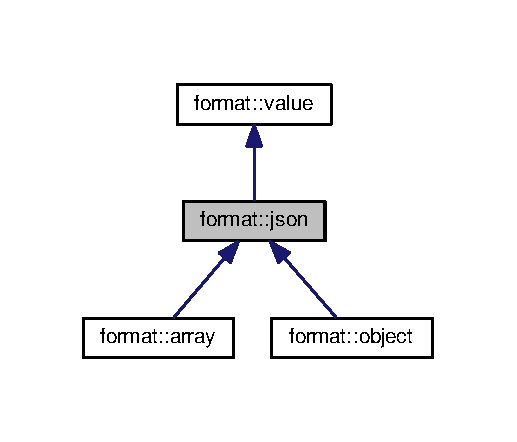
\includegraphics[width=248pt]{classformat_1_1json__inherit__graph}
\end{center}
\end{figure}


Collaboration diagram for format\+:\+:json\+:
\nopagebreak
\begin{figure}[H]
\begin{center}
\leavevmode
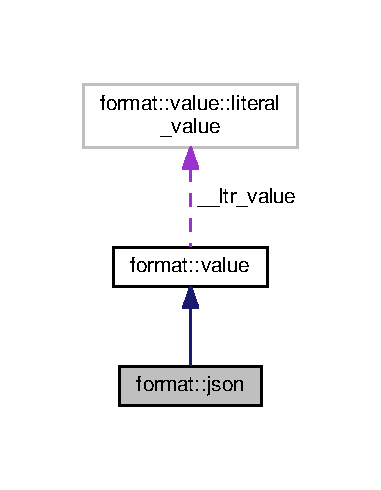
\includegraphics[width=183pt]{classformat_1_1json__coll__graph}
\end{center}
\end{figure}
\subsection*{Public Member Functions}
\begin{DoxyCompactItemize}
\item 
\hyperlink{classformat_1_1json_a076a6ac427f4c24ce8615e0d86f3bf72}{json} ()\hypertarget{classformat_1_1json_a076a6ac427f4c24ce8615e0d86f3bf72}{}\label{classformat_1_1json_a076a6ac427f4c24ce8615e0d86f3bf72}

\begin{DoxyCompactList}\small\item\em json \end{DoxyCompactList}\item 
\hyperlink{classformat_1_1json_a68e9a5bd2797f98f769f327840f30102}{json} (const wchar\+\_\+t $\ast$\hyperlink{classformat_1_1json}{json})
\begin{DoxyCompactList}\small\item\em json \end{DoxyCompactList}\item 
\hyperlink{classformat_1_1json_aeb56e34d244caf2e4a05d9133b938ab0}{json} (\hyperlink{classformat_1_1object}{object} $\ast$o)
\begin{DoxyCompactList}\small\item\em json \end{DoxyCompactList}\item 
\hyperlink{classformat_1_1json_afc70965bc62c2d30bba3bea65da83032}{json} (\hyperlink{classformat_1_1array}{array} $\ast$a)
\begin{DoxyCompactList}\small\item\em json \end{DoxyCompactList}\item 
\hyperlink{classformat_1_1json_a6d5df3e615981da43a79744ff6c6df00}{json} (const \hyperlink{classformat_1_1json}{json} \&other)
\begin{DoxyCompactList}\small\item\em json \end{DoxyCompactList}\item 
virtual \hyperlink{classformat_1_1json_abd5dba4e20afebd5677e935f5f56c14e}{$\sim$json} () override\hypertarget{classformat_1_1json_abd5dba4e20afebd5677e935f5f56c14e}{}\label{classformat_1_1json_abd5dba4e20afebd5677e935f5f56c14e}

\begin{DoxyCompactList}\small\item\em $\sim$json \end{DoxyCompactList}\item 
virtual \hyperlink{classformat_1_1value_aa6b85823936bf7b8ab78d3f8d443c00d}{value} $\ast$ \hyperlink{classformat_1_1json_a49534b733831b2dae879d7407f7cfba5}{clone} () const 
\begin{DoxyCompactList}\small\item\em clone \end{DoxyCompactList}\item 
virtual \hyperlink{classformat_1_1value_aa0334be06389a7b14af485fa0cd3aa21}{value\+::value\+\_\+t} \hyperlink{classformat_1_1json_a970027799aac71bf99e3f1d7264364dc}{type} () const noexceptoverride
\begin{DoxyCompactList}\small\item\em type \end{DoxyCompactList}\item 
virtual size\+\_\+t \hyperlink{classformat_1_1json_a792f3755d148f250ae60e4bbb35fbc6b}{length} () const noexceptoverride
\begin{DoxyCompactList}\small\item\em size \end{DoxyCompactList}\item 
\hyperlink{classformat_1_1value_aa6b85823936bf7b8ab78d3f8d443c00d}{value} \& \hyperlink{classformat_1_1json_a5bc59d792602f7c7f4211db5dfd67267}{\+\_\+assign} (const \hyperlink{classformat_1_1json}{json} \&j)
\begin{DoxyCompactList}\small\item\em \+\_\+assign \end{DoxyCompactList}\item 
\hyperlink{classformat_1_1value_aa6b85823936bf7b8ab78d3f8d443c00d}{value} \& \hyperlink{classformat_1_1json_a529a9a8bee8ae66f0cfd9757dd6744db}{operator=} (const \hyperlink{classformat_1_1json}{json} \&j)
\begin{DoxyCompactList}\small\item\em operator = \end{DoxyCompactList}\item 
virtual \hyperlink{classformat_1_1value_aa6b85823936bf7b8ab78d3f8d443c00d}{value} \& \hyperlink{classformat_1_1json_a331d385e55541671d431d5e5167e8c90}{\+\_\+assign} (\hyperlink{classformat_1_1value_aa6b85823936bf7b8ab78d3f8d443c00d}{value} $\ast$, \hyperlink{classformat_1_1value_aa6b85823936bf7b8ab78d3f8d443c00d}{value} $\ast$) override
\begin{DoxyCompactList}\small\item\em assign \end{DoxyCompactList}\item 
virtual size\+\_\+t \hyperlink{classformat_1_1json_a1110e453dd28d55ed9b6b196d04d1c7e}{str\+\_\+length} () const noexceptoverride
\begin{DoxyCompactList}\small\item\em str\+Length \end{DoxyCompactList}\end{DoxyCompactItemize}
\subsection*{Static Public Member Functions}
\begin{DoxyCompactItemize}
\item 
static \hyperlink{classformat_1_1value_aa6b85823936bf7b8ab78d3f8d443c00d}{value} $\ast$ \hyperlink{classformat_1_1json_ad99f1cac9b2ae0d67214228a4fd2469b}{parse} (const wchar\+\_\+t $\ast$text, reviver r=0)
\begin{DoxyCompactList}\small\item\em parse \end{DoxyCompactList}\end{DoxyCompactItemize}
\subsection*{Protected Member Functions}
\begin{DoxyCompactItemize}
\item 
\hyperlink{classformat_1_1json_a68a4f53726787a747982f6776d5c3086}{json} (\hyperlink{classformat_1_1json}{json} $\ast$\hyperlink{classformat_1_1value_a86c03ec8810bfd0d60ec49095120040d}{parent})
\begin{DoxyCompactList}\small\item\em json \end{DoxyCompactList}\item 
\hyperlink{classformat_1_1json_a76747146e785595b4c24d021feb8c5c0}{json} (const wchar\+\_\+t $\ast$\hyperlink{classformat_1_1json}{json}, const bool \+\_\+call\+\_\+parse)
\begin{DoxyCompactList}\small\item\em json \end{DoxyCompactList}\item 
virtual const wchar\+\_\+t $\ast$ \hyperlink{classformat_1_1json_ab316c1d4c585610a60d634605a4b871e}{\+\_\+parse} (const wchar\+\_\+t $\ast$readp) override
\begin{DoxyCompactList}\small\item\em parse \end{DoxyCompactList}\item 
virtual \hyperlink{classformat_1_1value_aa6b85823936bf7b8ab78d3f8d443c00d}{value} \& \hyperlink{classformat_1_1json_afcb78dfb597d7d609c66a4d5b6575082}{\+\_\+at} (const wchar\+\_\+t $\ast$\hyperlink{classformat_1_1value_ad4865e7984fc9f3b5ce7c17fd7ac740c}{key}) override
\begin{DoxyCompactList}\small\item\em \+\_\+at \end{DoxyCompactList}\item 
virtual \hyperlink{classformat_1_1value_aa6b85823936bf7b8ab78d3f8d443c00d}{value} \& \hyperlink{classformat_1_1json_a4a3924d5a112cda2bcee45ddf92a3d52}{\+\_\+at} (size\+\_\+t \hyperlink{classformat_1_1value_aaa429b28cc0edf5a3589b89a1820ad62}{index}) override
\begin{DoxyCompactList}\small\item\em \+\_\+at \end{DoxyCompactList}\item 
\hyperlink{classformat_1_1value_aa6b85823936bf7b8ab78d3f8d443c00d}{value} $\ast$ \hyperlink{classformat_1_1json_ae44c43633cd5cf6fbae535cb622ec778}{\+\_\+make\+\_\+value} ()
\begin{DoxyCompactList}\small\item\em \+\_\+make\+\_\+value \end{DoxyCompactList}\item 
{\footnotesize template$<$typename T $>$ }\\void \hyperlink{classformat_1_1json_ad26c343d5b9bcaf6f19b6049bfe2a7e7}{\+\_\+from\+\_\+initializer\+\_\+list} ()\hypertarget{classformat_1_1json_ad26c343d5b9bcaf6f19b6049bfe2a7e7}{}\label{classformat_1_1json_ad26c343d5b9bcaf6f19b6049bfe2a7e7}

\begin{DoxyCompactList}\small\item\em \+\_\+from\+\_\+initializer\+\_\+list \end{DoxyCompactList}\item 
virtual void \hyperlink{classformat_1_1json_add5e23fba3d384156bc3eadc1207c6ac}{\+\_\+clear} () override\hypertarget{classformat_1_1json_add5e23fba3d384156bc3eadc1207c6ac}{}\label{classformat_1_1json_add5e23fba3d384156bc3eadc1207c6ac}

\begin{DoxyCompactList}\small\item\em \+\_\+clear \end{DoxyCompactList}\item 
virtual \hyperlink{classformat_1_1value_aa6b85823936bf7b8ab78d3f8d443c00d}{value} $\ast$ \hyperlink{classformat_1_1json_a4da6b9a624017973c5955d840e61fdb7}{\+\_\+clone} (const \hyperlink{classformat_1_1value_aa6b85823936bf7b8ab78d3f8d443c00d}{value} \&) override
\begin{DoxyCompactList}\small\item\em \+\_\+clone \end{DoxyCompactList}\item 
virtual const wchar\+\_\+t $\ast$ \hyperlink{classformat_1_1json_afbb5d88bc2005d89b287e05d89fb2e06}{\+\_\+to\+\_\+string} (wchar\+\_\+t $\ast$offset=0) const override
\begin{DoxyCompactList}\small\item\em str\+Value \end{DoxyCompactList}\item 
virtual \hyperlink{classformat_1_1value_aa6b85823936bf7b8ab78d3f8d443c00d}{value} \& \hyperlink{classformat_1_1json_adfc8837bee40c5a11809717f8d34b192}{\+\_\+erase} (const \hyperlink{classformat_1_1value_aa6b85823936bf7b8ab78d3f8d443c00d}{value} \&v) noexceptoverride
\begin{DoxyCompactList}\small\item\em erase \end{DoxyCompactList}\item 
\hyperlink{classformat_1_1value_aa6b85823936bf7b8ab78d3f8d443c00d}{value} $\ast$ \hyperlink{classformat_1_1json_af4314003df90a7cf9e4da35b57946296}{\+\_\+call\+\_\+reviver} (\hyperlink{classformat_1_1value_aa6b85823936bf7b8ab78d3f8d443c00d}{value} $\ast$v, const wchar\+\_\+t $\ast$\hyperlink{classformat_1_1value_ad4865e7984fc9f3b5ce7c17fd7ac740c}{key}, size\+\_\+t \hyperlink{classformat_1_1value_aaa429b28cc0edf5a3589b89a1820ad62}{index}=0) const 
\begin{DoxyCompactList}\small\item\em \+\_\+call\+\_\+reviver \end{DoxyCompactList}\end{DoxyCompactItemize}
\subsection*{Protected Attributes}
\begin{DoxyCompactItemize}
\item 
wchar\+\_\+t $\ast$ \hyperlink{classformat_1_1json_a7cbc0a4205de011312fac90ccc097b9f}{\+\_\+str\+\_\+value} \mbox{[}2\mbox{]}\hypertarget{classformat_1_1json_a7cbc0a4205de011312fac90ccc097b9f}{}\label{classformat_1_1json_a7cbc0a4205de011312fac90ccc097b9f}

\begin{DoxyCompactList}\small\item\em \+\_\+str\+\_\+value \end{DoxyCompactList}\end{DoxyCompactItemize}
\subsection*{Additional Inherited Members}


\subsection{Detailed Description}
The json class. 

\subsection{Constructor \& Destructor Documentation}
\index{format\+::json@{format\+::json}!json@{json}}
\index{json@{json}!format\+::json@{format\+::json}}
\subsubsection[{\texorpdfstring{json(const wchar\+\_\+t $\ast$json)}{json(const wchar_t *json)}}]{\setlength{\rightskip}{0pt plus 5cm}format\+::json\+::json (
\begin{DoxyParamCaption}
\item[{const wchar\+\_\+t $\ast$}]{json}
\end{DoxyParamCaption}
)}\hypertarget{classformat_1_1json_a68e9a5bd2797f98f769f327840f30102}{}\label{classformat_1_1json_a68e9a5bd2797f98f769f327840f30102}


json 


\begin{DoxyParams}{Parameters}
{\em json} & \\
\hline
\end{DoxyParams}
\index{format\+::json@{format\+::json}!json@{json}}
\index{json@{json}!format\+::json@{format\+::json}}
\subsubsection[{\texorpdfstring{json(object $\ast$o)}{json(object *o)}}]{\setlength{\rightskip}{0pt plus 5cm}format\+::json\+::json (
\begin{DoxyParamCaption}
\item[{{\bf object} $\ast$}]{o}
\end{DoxyParamCaption}
)}\hypertarget{classformat_1_1json_aeb56e34d244caf2e4a05d9133b938ab0}{}\label{classformat_1_1json_aeb56e34d244caf2e4a05d9133b938ab0}


json 


\begin{DoxyParams}{Parameters}
{\em o} & \\
\hline
\end{DoxyParams}
\index{format\+::json@{format\+::json}!json@{json}}
\index{json@{json}!format\+::json@{format\+::json}}
\subsubsection[{\texorpdfstring{json(array $\ast$a)}{json(array *a)}}]{\setlength{\rightskip}{0pt plus 5cm}format\+::json\+::json (
\begin{DoxyParamCaption}
\item[{{\bf array} $\ast$}]{a}
\end{DoxyParamCaption}
)}\hypertarget{classformat_1_1json_afc70965bc62c2d30bba3bea65da83032}{}\label{classformat_1_1json_afc70965bc62c2d30bba3bea65da83032}


json 


\begin{DoxyParams}{Parameters}
{\em a} & \\
\hline
\end{DoxyParams}
\index{format\+::json@{format\+::json}!json@{json}}
\index{json@{json}!format\+::json@{format\+::json}}
\subsubsection[{\texorpdfstring{json(const json \&other)}{json(const json &other)}}]{\setlength{\rightskip}{0pt plus 5cm}format\+::json\+::json (
\begin{DoxyParamCaption}
\item[{const {\bf json} \&}]{other}
\end{DoxyParamCaption}
)}\hypertarget{classformat_1_1json_a6d5df3e615981da43a79744ff6c6df00}{}\label{classformat_1_1json_a6d5df3e615981da43a79744ff6c6df00}


json 


\begin{DoxyParams}{Parameters}
{\em other} & \\
\hline
\end{DoxyParams}
\index{format\+::json@{format\+::json}!json@{json}}
\index{json@{json}!format\+::json@{format\+::json}}
\subsubsection[{\texorpdfstring{json(json $\ast$parent)}{json(json *parent)}}]{\setlength{\rightskip}{0pt plus 5cm}format\+::json\+::json (
\begin{DoxyParamCaption}
\item[{{\bf json} $\ast$}]{parent}
\end{DoxyParamCaption}
)\hspace{0.3cm}{\ttfamily [protected]}}\hypertarget{classformat_1_1json_a68a4f53726787a747982f6776d5c3086}{}\label{classformat_1_1json_a68a4f53726787a747982f6776d5c3086}


json 


\begin{DoxyParams}{Parameters}
{\em parent} & \\
\hline
\end{DoxyParams}
\index{format\+::json@{format\+::json}!json@{json}}
\index{json@{json}!format\+::json@{format\+::json}}
\subsubsection[{\texorpdfstring{json(const wchar\+\_\+t $\ast$json, const bool \+\_\+call\+\_\+parse)}{json(const wchar_t *json, const bool _call_parse)}}]{\setlength{\rightskip}{0pt plus 5cm}format\+::json\+::json (
\begin{DoxyParamCaption}
\item[{const wchar\+\_\+t $\ast$}]{json, }
\item[{const bool}]{\+\_\+call\+\_\+parse}
\end{DoxyParamCaption}
)\hspace{0.3cm}{\ttfamily [protected]}}\hypertarget{classformat_1_1json_a76747146e785595b4c24d021feb8c5c0}{}\label{classformat_1_1json_a76747146e785595b4c24d021feb8c5c0}


json 


\begin{DoxyParams}{Parameters}
{\em json} & \\
\hline
{\em \+\_\+call\+\_\+parse} & \\
\hline
\end{DoxyParams}


\subsection{Member Function Documentation}
\index{format\+::json@{format\+::json}!\+\_\+assign@{\+\_\+assign}}
\index{\+\_\+assign@{\+\_\+assign}!format\+::json@{format\+::json}}
\subsubsection[{\texorpdfstring{\+\_\+assign(const json \&j)}{_assign(const json &j)}}]{\setlength{\rightskip}{0pt plus 5cm}{\bf format\+::value} \& format\+::json\+::\+\_\+assign (
\begin{DoxyParamCaption}
\item[{const {\bf json} \&}]{j}
\end{DoxyParamCaption}
)}\hypertarget{classformat_1_1json_a5bc59d792602f7c7f4211db5dfd67267}{}\label{classformat_1_1json_a5bc59d792602f7c7f4211db5dfd67267}


\+\_\+assign 


\begin{DoxyParams}{Parameters}
{\em j} & \\
\hline
\end{DoxyParams}
\begin{DoxyReturn}{Returns}

\end{DoxyReturn}
\index{format\+::json@{format\+::json}!\+\_\+assign@{\+\_\+assign}}
\index{\+\_\+assign@{\+\_\+assign}!format\+::json@{format\+::json}}
\subsubsection[{\texorpdfstring{\+\_\+assign(value $\ast$, value $\ast$) override}{_assign(value *, value *) override}}]{\setlength{\rightskip}{0pt plus 5cm}virtual {\bf value}\& format\+::json\+::\+\_\+assign (
\begin{DoxyParamCaption}
\item[{{\bf value} $\ast$}]{, }
\item[{{\bf value} $\ast$}]{}
\end{DoxyParamCaption}
)\hspace{0.3cm}{\ttfamily [inline]}, {\ttfamily [override]}, {\ttfamily [virtual]}}\hypertarget{classformat_1_1json_a331d385e55541671d431d5e5167e8c90}{}\label{classformat_1_1json_a331d385e55541671d431d5e5167e8c90}


assign 


\begin{DoxyParams}{Parameters}
{\em ov} & Old value \\
\hline
{\em nv} & New value \\
\hline
\end{DoxyParams}
\begin{DoxyReturn}{Returns}

\end{DoxyReturn}


Reimplemented in \hyperlink{classformat_1_1object_ad1b5cd15cd7db0d3afba5ec5fa713a1e}{format\+::object}, and \hyperlink{classformat_1_1array_a4407859f08e94c0d761dffd6eb4578f6}{format\+::array}.

\index{format\+::json@{format\+::json}!\+\_\+at@{\+\_\+at}}
\index{\+\_\+at@{\+\_\+at}!format\+::json@{format\+::json}}
\subsubsection[{\texorpdfstring{\+\_\+at(const wchar\+\_\+t $\ast$key) override}{_at(const wchar_t *key) override}}]{\setlength{\rightskip}{0pt plus 5cm}{\bf format\+::value} \& format\+::json\+::\+\_\+at (
\begin{DoxyParamCaption}
\item[{const wchar\+\_\+t $\ast$}]{key}
\end{DoxyParamCaption}
)\hspace{0.3cm}{\ttfamily [override]}, {\ttfamily [protected]}, {\ttfamily [virtual]}}\hypertarget{classformat_1_1json_afcb78dfb597d7d609c66a4d5b6575082}{}\label{classformat_1_1json_afcb78dfb597d7d609c66a4d5b6575082}


\+\_\+at 


\begin{DoxyParams}{Parameters}
{\em key} & \\
\hline
\end{DoxyParams}
\begin{DoxyReturn}{Returns}

\end{DoxyReturn}


Implements \hyperlink{classformat_1_1value_a3f67662acb201f2ab8a768f8cb670678}{format\+::value}.



Reimplemented in \hyperlink{classformat_1_1object_a91e3027c7786c2e24ca3e001f648542d}{format\+::object}, and \hyperlink{classformat_1_1array_a6e6822294f55273f657732d048aa38f8}{format\+::array}.

\index{format\+::json@{format\+::json}!\+\_\+at@{\+\_\+at}}
\index{\+\_\+at@{\+\_\+at}!format\+::json@{format\+::json}}
\subsubsection[{\texorpdfstring{\+\_\+at(size\+\_\+t index) override}{_at(size_t index) override}}]{\setlength{\rightskip}{0pt plus 5cm}{\bf format\+::value} \& format\+::json\+::\+\_\+at (
\begin{DoxyParamCaption}
\item[{size\+\_\+t}]{index}
\end{DoxyParamCaption}
)\hspace{0.3cm}{\ttfamily [override]}, {\ttfamily [protected]}, {\ttfamily [virtual]}}\hypertarget{classformat_1_1json_a4a3924d5a112cda2bcee45ddf92a3d52}{}\label{classformat_1_1json_a4a3924d5a112cda2bcee45ddf92a3d52}


\+\_\+at 


\begin{DoxyParams}{Parameters}
{\em index} & \\
\hline
\end{DoxyParams}
\begin{DoxyReturn}{Returns}

\end{DoxyReturn}


Implements \hyperlink{classformat_1_1value_ab94a7f0af8ea5c60fd0e59ccde8d0371}{format\+::value}.



Reimplemented in \hyperlink{classformat_1_1object_a525bdfa2db22cd6bc21a868a695fe752}{format\+::object}, and \hyperlink{classformat_1_1array_a386fd4c0f2556459186db7f22df4128e}{format\+::array}.

\index{format\+::json@{format\+::json}!\+\_\+call\+\_\+reviver@{\+\_\+call\+\_\+reviver}}
\index{\+\_\+call\+\_\+reviver@{\+\_\+call\+\_\+reviver}!format\+::json@{format\+::json}}
\subsubsection[{\texorpdfstring{\+\_\+call\+\_\+reviver(value $\ast$v, const wchar\+\_\+t $\ast$key, size\+\_\+t index=0) const }{_call_reviver(value *v, const wchar_t *key, size_t index=0) const }}]{\setlength{\rightskip}{0pt plus 5cm}{\bf format\+::value} $\ast$ format\+::json\+::\+\_\+call\+\_\+reviver (
\begin{DoxyParamCaption}
\item[{{\bf value} $\ast$}]{v, }
\item[{const wchar\+\_\+t $\ast$}]{key, }
\item[{size\+\_\+t}]{index = {\ttfamily 0}}
\end{DoxyParamCaption}
) const\hspace{0.3cm}{\ttfamily [protected]}}\hypertarget{classformat_1_1json_af4314003df90a7cf9e4da35b57946296}{}\label{classformat_1_1json_af4314003df90a7cf9e4da35b57946296}


\+\_\+call\+\_\+reviver 


\begin{DoxyParams}{Parameters}
{\em v} & \\
\hline
{\em key} & \\
\hline
{\em index} & \\
\hline
\end{DoxyParams}
\begin{DoxyReturn}{Returns}

\end{DoxyReturn}
\index{format\+::json@{format\+::json}!\+\_\+clone@{\+\_\+clone}}
\index{\+\_\+clone@{\+\_\+clone}!format\+::json@{format\+::json}}
\subsubsection[{\texorpdfstring{\+\_\+clone(const value \&) override}{_clone(const value &) override}}]{\setlength{\rightskip}{0pt plus 5cm}virtual {\bf value}$\ast$ format\+::json\+::\+\_\+clone (
\begin{DoxyParamCaption}
\item[{const {\bf value} \&}]{}
\end{DoxyParamCaption}
)\hspace{0.3cm}{\ttfamily [inline]}, {\ttfamily [override]}, {\ttfamily [protected]}, {\ttfamily [virtual]}}\hypertarget{classformat_1_1json_a4da6b9a624017973c5955d840e61fdb7}{}\label{classformat_1_1json_a4da6b9a624017973c5955d840e61fdb7}


\+\_\+clone 

\begin{DoxyReturn}{Returns}

\end{DoxyReturn}


Reimplemented in \hyperlink{classformat_1_1array_abd0469398fdb7eed92ef3b785a94ae8f}{format\+::array}, and \hyperlink{classformat_1_1object_ad0de8290132a916e810df0819f6400cb}{format\+::object}.

\index{format\+::json@{format\+::json}!\+\_\+erase@{\+\_\+erase}}
\index{\+\_\+erase@{\+\_\+erase}!format\+::json@{format\+::json}}
\subsubsection[{\texorpdfstring{\+\_\+erase(const value \&v) noexceptoverride}{_erase(const value &v) noexceptoverride}}]{\setlength{\rightskip}{0pt plus 5cm}virtual {\bf value}\& format\+::json\+::\+\_\+erase (
\begin{DoxyParamCaption}
\item[{const {\bf value} \&}]{v}
\end{DoxyParamCaption}
)\hspace{0.3cm}{\ttfamily [inline]}, {\ttfamily [override]}, {\ttfamily [protected]}, {\ttfamily [virtual]}, {\ttfamily [noexcept]}}\hypertarget{classformat_1_1json_adfc8837bee40c5a11809717f8d34b192}{}\label{classformat_1_1json_adfc8837bee40c5a11809717f8d34b192}


erase 


\begin{DoxyParams}{Parameters}
{\em v} & \\
\hline
\end{DoxyParams}
\begin{DoxyReturn}{Returns}

\end{DoxyReturn}


Reimplemented in \hyperlink{classformat_1_1object_a8da91a2e94cea219e1462d7857f27af7}{format\+::object}, and \hyperlink{classformat_1_1array_a543a2cf1adc8ff7f91eea7ea881c0247}{format\+::array}.

\index{format\+::json@{format\+::json}!\+\_\+make\+\_\+value@{\+\_\+make\+\_\+value}}
\index{\+\_\+make\+\_\+value@{\+\_\+make\+\_\+value}!format\+::json@{format\+::json}}
\subsubsection[{\texorpdfstring{\+\_\+make\+\_\+value()}{_make_value()}}]{\setlength{\rightskip}{0pt plus 5cm}{\bf format\+::value} $\ast$ format\+::json\+::\+\_\+make\+\_\+value (
\begin{DoxyParamCaption}
{}
\end{DoxyParamCaption}
)\hspace{0.3cm}{\ttfamily [protected]}}\hypertarget{classformat_1_1json_ae44c43633cd5cf6fbae535cb622ec778}{}\label{classformat_1_1json_ae44c43633cd5cf6fbae535cb622ec778}


\+\_\+make\+\_\+value 

\begin{DoxyReturn}{Returns}

\end{DoxyReturn}
\index{format\+::json@{format\+::json}!\+\_\+parse@{\+\_\+parse}}
\index{\+\_\+parse@{\+\_\+parse}!format\+::json@{format\+::json}}
\subsubsection[{\texorpdfstring{\+\_\+parse(const wchar\+\_\+t $\ast$readp) override}{_parse(const wchar_t *readp) override}}]{\setlength{\rightskip}{0pt plus 5cm}virtual const wchar\+\_\+t$\ast$ format\+::json\+::\+\_\+parse (
\begin{DoxyParamCaption}
\item[{const wchar\+\_\+t $\ast$}]{readp}
\end{DoxyParamCaption}
)\hspace{0.3cm}{\ttfamily [override]}, {\ttfamily [protected]}, {\ttfamily [virtual]}}\hypertarget{classformat_1_1json_ab316c1d4c585610a60d634605a4b871e}{}\label{classformat_1_1json_ab316c1d4c585610a60d634605a4b871e}


parse 


\begin{DoxyParams}{Parameters}
{\em readp} & \\
\hline
\end{DoxyParams}
\begin{DoxyReturn}{Returns}

\end{DoxyReturn}


Implements \hyperlink{classformat_1_1value_a7859b1aa48f667a83e091f0eba22d4a1}{format\+::value}.



Reimplemented in \hyperlink{classformat_1_1object_a6680c7e4b32da5a29d89f2289bb63ee1}{format\+::object}, and \hyperlink{classformat_1_1array_a7bd1454afcf365128e2a5db112b2895f}{format\+::array}.

\index{format\+::json@{format\+::json}!\+\_\+to\+\_\+string@{\+\_\+to\+\_\+string}}
\index{\+\_\+to\+\_\+string@{\+\_\+to\+\_\+string}!format\+::json@{format\+::json}}
\subsubsection[{\texorpdfstring{\+\_\+to\+\_\+string(wchar\+\_\+t $\ast$offset=0) const override}{_to_string(wchar_t *offset=0) const override}}]{\setlength{\rightskip}{0pt plus 5cm}virtual const wchar\+\_\+t$\ast$ format\+::json\+::\+\_\+to\+\_\+string (
\begin{DoxyParamCaption}
\item[{wchar\+\_\+t $\ast$}]{offset = {\ttfamily 0}}
\end{DoxyParamCaption}
) const\hspace{0.3cm}{\ttfamily [inline]}, {\ttfamily [override]}, {\ttfamily [protected]}, {\ttfamily [virtual]}}\hypertarget{classformat_1_1json_afbb5d88bc2005d89b287e05d89fb2e06}{}\label{classformat_1_1json_afbb5d88bc2005d89b287e05d89fb2e06}


str\+Value 

\begin{DoxyReturn}{Returns}

\end{DoxyReturn}


Implements \hyperlink{classformat_1_1value_a94ed31f07b19866495297472accd33a8}{format\+::value}.



Reimplemented in \hyperlink{classformat_1_1object_ade521091c997a1a61e15122364c32e99}{format\+::object}, and \hyperlink{classformat_1_1array_a3a8da80fceac963967b0d6d08a69ed18}{format\+::array}.

\index{format\+::json@{format\+::json}!clone@{clone}}
\index{clone@{clone}!format\+::json@{format\+::json}}
\subsubsection[{\texorpdfstring{clone() const }{clone() const }}]{\setlength{\rightskip}{0pt plus 5cm}virtual {\bf value}$\ast$ format\+::json\+::clone (
\begin{DoxyParamCaption}
{}
\end{DoxyParamCaption}
) const\hspace{0.3cm}{\ttfamily [inline]}, {\ttfamily [virtual]}}\hypertarget{classformat_1_1json_a49534b733831b2dae879d7407f7cfba5}{}\label{classformat_1_1json_a49534b733831b2dae879d7407f7cfba5}


clone 

\begin{DoxyReturn}{Returns}

\end{DoxyReturn}


Implements \hyperlink{classformat_1_1value_a8756eb79e41851859d83ae46069dc400}{format\+::value}.



Reimplemented in \hyperlink{classformat_1_1array_a456f53d9b5049e9af8d28b9588fc61c4}{format\+::array}, and \hyperlink{classformat_1_1object_a3e6550914c83ba0796877e5da8a511bd}{format\+::object}.

\index{format\+::json@{format\+::json}!length@{length}}
\index{length@{length}!format\+::json@{format\+::json}}
\subsubsection[{\texorpdfstring{length() const noexceptoverride}{length() const noexceptoverride}}]{\setlength{\rightskip}{0pt plus 5cm}virtual size\+\_\+t format\+::json\+::length (
\begin{DoxyParamCaption}
{}
\end{DoxyParamCaption}
) const\hspace{0.3cm}{\ttfamily [inline]}, {\ttfamily [override]}, {\ttfamily [virtual]}, {\ttfamily [noexcept]}}\hypertarget{classformat_1_1json_a792f3755d148f250ae60e4bbb35fbc6b}{}\label{classformat_1_1json_a792f3755d148f250ae60e4bbb35fbc6b}


size 

\begin{DoxyReturn}{Returns}

\end{DoxyReturn}


Implements \hyperlink{classformat_1_1value_a406a9553c4d83a0613aa54d77f6c462d}{format\+::value}.



Reimplemented in \hyperlink{classformat_1_1array_af15910f0535e266984f3f745efae5397}{format\+::array}, and \hyperlink{classformat_1_1object_a29be05a1b87c2d6263f15fc3280e3b6f}{format\+::object}.

\index{format\+::json@{format\+::json}!operator=@{operator=}}
\index{operator=@{operator=}!format\+::json@{format\+::json}}
\subsubsection[{\texorpdfstring{operator=(const json \&j)}{operator=(const json &j)}}]{\setlength{\rightskip}{0pt plus 5cm}{\bf value}\& format\+::json\+::operator= (
\begin{DoxyParamCaption}
\item[{const {\bf json} \&}]{j}
\end{DoxyParamCaption}
)\hspace{0.3cm}{\ttfamily [inline]}}\hypertarget{classformat_1_1json_a529a9a8bee8ae66f0cfd9757dd6744db}{}\label{classformat_1_1json_a529a9a8bee8ae66f0cfd9757dd6744db}


operator = 


\begin{DoxyParams}{Parameters}
{\em j} & \\
\hline
\end{DoxyParams}
\begin{DoxyReturn}{Returns}

\end{DoxyReturn}
\index{format\+::json@{format\+::json}!parse@{parse}}
\index{parse@{parse}!format\+::json@{format\+::json}}
\subsubsection[{\texorpdfstring{parse(const wchar\+\_\+t $\ast$text, reviver r=0)}{parse(const wchar_t *text, reviver r=0)}}]{\setlength{\rightskip}{0pt plus 5cm}static {\bf value}$\ast$ format\+::json\+::parse (
\begin{DoxyParamCaption}
\item[{const wchar\+\_\+t $\ast$}]{text, }
\item[{reviver}]{r = {\ttfamily 0}}
\end{DoxyParamCaption}
)\hspace{0.3cm}{\ttfamily [inline]}, {\ttfamily [static]}}\hypertarget{classformat_1_1json_ad99f1cac9b2ae0d67214228a4fd2469b}{}\label{classformat_1_1json_ad99f1cac9b2ae0d67214228a4fd2469b}


parse 


\begin{DoxyParams}{Parameters}
{\em json} & \\
\hline
{\em reviver} & \\
\hline
\end{DoxyParams}
\begin{DoxyReturn}{Returns}

\end{DoxyReturn}
\begin{DoxySeeAlso}{See also}
\href{http://stackoverflow.com/questions/1174169/function-passed-as-template-argument}{\tt http\+://stackoverflow.\+com/questions/1174169/function-\/passed-\/as-\/template-\/argument} 
\end{DoxySeeAlso}
\index{format\+::json@{format\+::json}!str\+\_\+length@{str\+\_\+length}}
\index{str\+\_\+length@{str\+\_\+length}!format\+::json@{format\+::json}}
\subsubsection[{\texorpdfstring{str\+\_\+length() const noexceptoverride}{str_length() const noexceptoverride}}]{\setlength{\rightskip}{0pt plus 5cm}virtual size\+\_\+t format\+::json\+::str\+\_\+length (
\begin{DoxyParamCaption}
{}
\end{DoxyParamCaption}
) const\hspace{0.3cm}{\ttfamily [inline]}, {\ttfamily [override]}, {\ttfamily [virtual]}, {\ttfamily [noexcept]}}\hypertarget{classformat_1_1json_a1110e453dd28d55ed9b6b196d04d1c7e}{}\label{classformat_1_1json_a1110e453dd28d55ed9b6b196d04d1c7e}


str\+Length 

\begin{DoxyReturn}{Returns}

\end{DoxyReturn}


Implements \hyperlink{classformat_1_1value_a399280e27e629db0582b5781b90ca58b}{format\+::value}.



Reimplemented in \hyperlink{classformat_1_1array_a579c320809545c627af0cbf9d8365080}{format\+::array}, and \hyperlink{classformat_1_1object_a866a470f6092172fcde8307882236a50}{format\+::object}.

\index{format\+::json@{format\+::json}!type@{type}}
\index{type@{type}!format\+::json@{format\+::json}}
\subsubsection[{\texorpdfstring{type() const noexceptoverride}{type() const noexceptoverride}}]{\setlength{\rightskip}{0pt plus 5cm}virtual {\bf value\+::value\+\_\+t} format\+::json\+::type (
\begin{DoxyParamCaption}
{}
\end{DoxyParamCaption}
) const\hspace{0.3cm}{\ttfamily [inline]}, {\ttfamily [override]}, {\ttfamily [virtual]}, {\ttfamily [noexcept]}}\hypertarget{classformat_1_1json_a970027799aac71bf99e3f1d7264364dc}{}\label{classformat_1_1json_a970027799aac71bf99e3f1d7264364dc}


type 

\begin{DoxyReturn}{Returns}

\end{DoxyReturn}


Implements \hyperlink{classformat_1_1value_a7112d0f83cf61aa9e1cdde90fc444996}{format\+::value}.



Reimplemented in \hyperlink{classformat_1_1array_a0fe16076f81ccc66e8208fe6dd4d2b1a}{format\+::array}, and \hyperlink{classformat_1_1object_aea7eb835fcbec62a85d078a7fa33cea7}{format\+::object}.



The documentation for this class was generated from the following files\+:\begin{DoxyCompactItemize}
\item 
json\+\_\+json.\+h\item 
json\+\_\+json.\+cpp\end{DoxyCompactItemize}

\hypertarget{classformat_1_1json__error}{}\section{format\+:\+:json\+\_\+error Class Reference}
\label{classformat_1_1json__error}\index{format\+::json\+\_\+error@{format\+::json\+\_\+error}}


The J\+S\+O\+N\+\_\+\+Error class.  




{\ttfamily \#include $<$json\+\_\+exception.\+h$>$}



Inheritance diagram for format\+:\+:json\+\_\+error\+:
\nopagebreak
\begin{figure}[H]
\begin{center}
\leavevmode
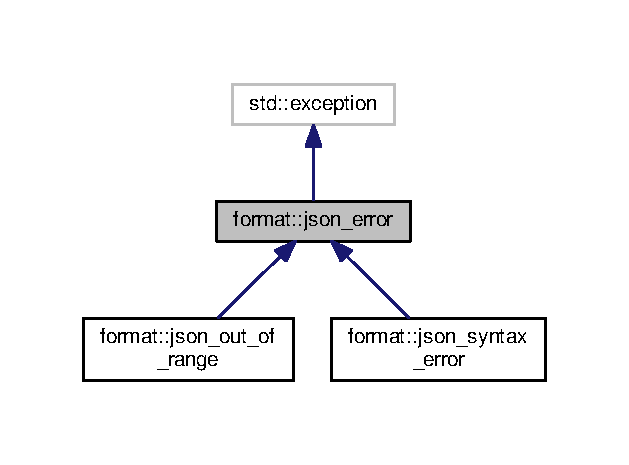
\includegraphics[width=302pt]{classformat_1_1json__error__inherit__graph}
\end{center}
\end{figure}


Collaboration diagram for format\+:\+:json\+\_\+error\+:
\nopagebreak
\begin{figure}[H]
\begin{center}
\leavevmode
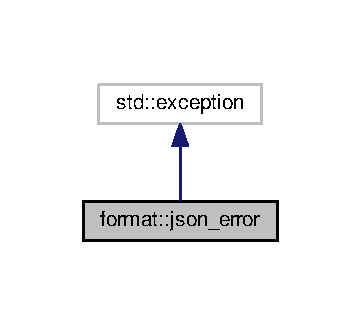
\includegraphics[width=173pt]{classformat_1_1json__error__coll__graph}
\end{center}
\end{figure}
\subsection*{Public Member Functions}
\begin{DoxyCompactItemize}
\item 
\hyperlink{classformat_1_1json__error_ad5f0a824e997a04144759e2e914bee96}{json\+\_\+error} (const char $\ast$const \hyperlink{classformat_1_1json__error_ad485f2d9233498b1a66695f94e313dd5}{what})
\begin{DoxyCompactList}\small\item\em J\+S\+O\+N\+\_\+\+Error. \end{DoxyCompactList}\item 
virtual const char $\ast$ \hyperlink{classformat_1_1json__error_ad485f2d9233498b1a66695f94e313dd5}{what} () const noexcept
\begin{DoxyCompactList}\small\item\em what \end{DoxyCompactList}\end{DoxyCompactItemize}
\subsection*{Protected Attributes}
\begin{DoxyCompactItemize}
\item 
std\+::string \hyperlink{classformat_1_1json__error_a7d924b7e8cacd89885cee0a398baaa6a}{\+\_\+what}\hypertarget{classformat_1_1json__error_a7d924b7e8cacd89885cee0a398baaa6a}{}\label{classformat_1_1json__error_a7d924b7e8cacd89885cee0a398baaa6a}

\begin{DoxyCompactList}\small\item\em \+\_\+what \end{DoxyCompactList}\end{DoxyCompactItemize}


\subsection{Detailed Description}
The J\+S\+O\+N\+\_\+\+Error class. 

\subsection{Constructor \& Destructor Documentation}
\index{format\+::json\+\_\+error@{format\+::json\+\_\+error}!json\+\_\+error@{json\+\_\+error}}
\index{json\+\_\+error@{json\+\_\+error}!format\+::json\+\_\+error@{format\+::json\+\_\+error}}
\subsubsection[{\texorpdfstring{json\+\_\+error(const char $\ast$const what)}{json_error(const char *const what)}}]{\setlength{\rightskip}{0pt plus 5cm}format\+::json\+\_\+error\+::json\+\_\+error (
\begin{DoxyParamCaption}
\item[{const char $\ast$const}]{what}
\end{DoxyParamCaption}
)\hspace{0.3cm}{\ttfamily [inline]}}\hypertarget{classformat_1_1json__error_ad5f0a824e997a04144759e2e914bee96}{}\label{classformat_1_1json__error_ad5f0a824e997a04144759e2e914bee96}


J\+S\+O\+N\+\_\+\+Error. 


\begin{DoxyParams}{Parameters}
{\em what} & \\
\hline
\end{DoxyParams}


\subsection{Member Function Documentation}
\index{format\+::json\+\_\+error@{format\+::json\+\_\+error}!what@{what}}
\index{what@{what}!format\+::json\+\_\+error@{format\+::json\+\_\+error}}
\subsubsection[{\texorpdfstring{what() const noexcept}{what() const noexcept}}]{\setlength{\rightskip}{0pt plus 5cm}virtual const char$\ast$ format\+::json\+\_\+error\+::what (
\begin{DoxyParamCaption}
{}
\end{DoxyParamCaption}
) const\hspace{0.3cm}{\ttfamily [inline]}, {\ttfamily [virtual]}, {\ttfamily [noexcept]}}\hypertarget{classformat_1_1json__error_ad485f2d9233498b1a66695f94e313dd5}{}\label{classformat_1_1json__error_ad485f2d9233498b1a66695f94e313dd5}


what 

\begin{DoxyReturn}{Returns}

\end{DoxyReturn}


The documentation for this class was generated from the following file\+:\begin{DoxyCompactItemize}
\item 
json\+\_\+exception.\+h\end{DoxyCompactItemize}

\hypertarget{classformat_1_1json__out__of__range}{}\section{format\+:\+:json\+\_\+out\+\_\+of\+\_\+range Class Reference}
\label{classformat_1_1json__out__of__range}\index{format\+::json\+\_\+out\+\_\+of\+\_\+range@{format\+::json\+\_\+out\+\_\+of\+\_\+range}}


The J\+S\+O\+N\+\_\+\+Out\+\_\+\+Of\+\_\+\+Range class.  




{\ttfamily \#include $<$json\+\_\+exception.\+h$>$}



Inheritance diagram for format\+:\+:json\+\_\+out\+\_\+of\+\_\+range\+:
\nopagebreak
\begin{figure}[H]
\begin{center}
\leavevmode
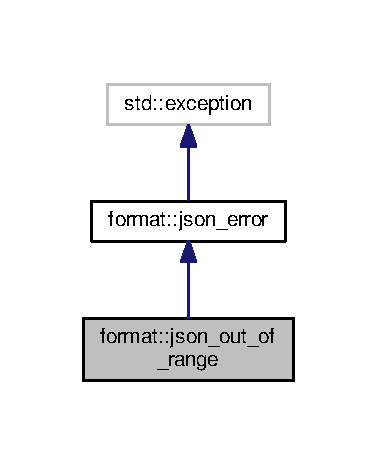
\includegraphics[width=181pt]{classformat_1_1json__out__of__range__inherit__graph}
\end{center}
\end{figure}


Collaboration diagram for format\+:\+:json\+\_\+out\+\_\+of\+\_\+range\+:
\nopagebreak
\begin{figure}[H]
\begin{center}
\leavevmode
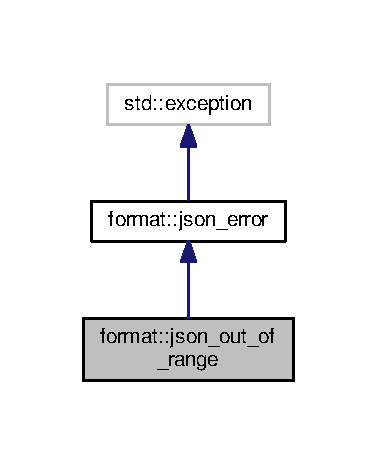
\includegraphics[width=181pt]{classformat_1_1json__out__of__range__coll__graph}
\end{center}
\end{figure}
\subsection*{Public Member Functions}
\begin{DoxyCompactItemize}
\item 
\hyperlink{classformat_1_1json__out__of__range_af742d359f531d819d43907c929a1f03b}{json\+\_\+out\+\_\+of\+\_\+range} (const char $\ast$const \hyperlink{classformat_1_1json__error_ad485f2d9233498b1a66695f94e313dd5}{what})
\begin{DoxyCompactList}\small\item\em Syntax\+\_\+\+Error. \end{DoxyCompactList}\end{DoxyCompactItemize}
\subsection*{Additional Inherited Members}


\subsection{Detailed Description}
The J\+S\+O\+N\+\_\+\+Out\+\_\+\+Of\+\_\+\+Range class. 

\subsection{Constructor \& Destructor Documentation}
\index{format\+::json\+\_\+out\+\_\+of\+\_\+range@{format\+::json\+\_\+out\+\_\+of\+\_\+range}!json\+\_\+out\+\_\+of\+\_\+range@{json\+\_\+out\+\_\+of\+\_\+range}}
\index{json\+\_\+out\+\_\+of\+\_\+range@{json\+\_\+out\+\_\+of\+\_\+range}!format\+::json\+\_\+out\+\_\+of\+\_\+range@{format\+::json\+\_\+out\+\_\+of\+\_\+range}}
\subsubsection[{\texorpdfstring{json\+\_\+out\+\_\+of\+\_\+range(const char $\ast$const what)}{json_out_of_range(const char *const what)}}]{\setlength{\rightskip}{0pt plus 5cm}format\+::json\+\_\+out\+\_\+of\+\_\+range\+::json\+\_\+out\+\_\+of\+\_\+range (
\begin{DoxyParamCaption}
\item[{const char $\ast$const}]{what}
\end{DoxyParamCaption}
)\hspace{0.3cm}{\ttfamily [inline]}}\hypertarget{classformat_1_1json__out__of__range_af742d359f531d819d43907c929a1f03b}{}\label{classformat_1_1json__out__of__range_af742d359f531d819d43907c929a1f03b}


Syntax\+\_\+\+Error. 


\begin{DoxyParams}{Parameters}
{\em what} & \\
\hline
\end{DoxyParams}


The documentation for this class was generated from the following file\+:\begin{DoxyCompactItemize}
\item 
json\+\_\+exception.\+h\end{DoxyCompactItemize}

\hypertarget{classformat_1_1json__syntax__error}{}\section{format\+:\+:json\+\_\+syntax\+\_\+error Class Reference}
\label{classformat_1_1json__syntax__error}\index{format\+::json\+\_\+syntax\+\_\+error@{format\+::json\+\_\+syntax\+\_\+error}}


The J\+S\+O\+N\+\_\+\+Syntax\+\_\+\+Error class.  




{\ttfamily \#include $<$json\+\_\+exception.\+h$>$}



Inheritance diagram for format\+:\+:json\+\_\+syntax\+\_\+error\+:
\nopagebreak
\begin{figure}[H]
\begin{center}
\leavevmode
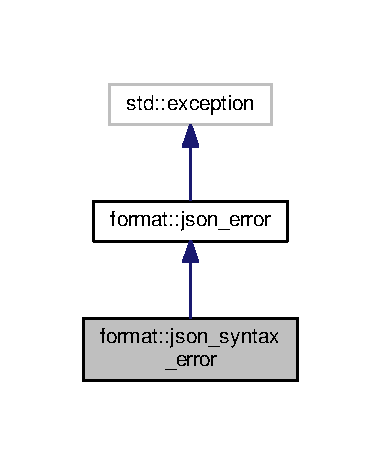
\includegraphics[width=183pt]{classformat_1_1json__syntax__error__inherit__graph}
\end{center}
\end{figure}


Collaboration diagram for format\+:\+:json\+\_\+syntax\+\_\+error\+:
\nopagebreak
\begin{figure}[H]
\begin{center}
\leavevmode
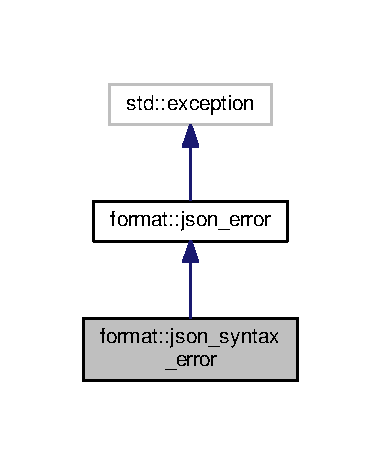
\includegraphics[width=183pt]{classformat_1_1json__syntax__error__coll__graph}
\end{center}
\end{figure}
\subsection*{Public Member Functions}
\begin{DoxyCompactItemize}
\item 
\hyperlink{classformat_1_1json__syntax__error_adc11f7d60bc9d8e69364205826df301b}{json\+\_\+syntax\+\_\+error} (const char $\ast$const \hyperlink{classformat_1_1json__error_ad485f2d9233498b1a66695f94e313dd5}{what})
\begin{DoxyCompactList}\small\item\em Syntax\+\_\+\+Error. \end{DoxyCompactList}\item 
\hyperlink{classformat_1_1json__syntax__error_a662ffb27c025c7934a57783a50b388df}{json\+\_\+syntax\+\_\+error} (const char $\ast$const \hyperlink{classformat_1_1json__error_ad485f2d9233498b1a66695f94e313dd5}{what}, wchar\+\_\+t token)
\begin{DoxyCompactList}\small\item\em Syntax\+\_\+\+Error. \end{DoxyCompactList}\item 
\hyperlink{classformat_1_1json__syntax__error_add967122801c06e55247d38bf1f5bef0}{json\+\_\+syntax\+\_\+error} (const char $\ast$const \hyperlink{classformat_1_1json__error_ad485f2d9233498b1a66695f94e313dd5}{what}, const wchar\+\_\+t $\ast$token, size\+\_\+t charc=0)
\begin{DoxyCompactList}\small\item\em Syntax\+\_\+\+Error. \end{DoxyCompactList}\end{DoxyCompactItemize}
\subsection*{Protected Member Functions}
\begin{DoxyCompactItemize}
\item 
size\+\_\+t {\bfseries \+\_\+add\+\_\+token} (const wchar\+\_\+t $\ast$token, size\+\_\+t charc=0)\hypertarget{classformat_1_1json__syntax__error_a3ed3b471ec7790e02a44176ad4ef64c3}{}\label{classformat_1_1json__syntax__error_a3ed3b471ec7790e02a44176ad4ef64c3}

\end{DoxyCompactItemize}
\subsection*{Additional Inherited Members}


\subsection{Detailed Description}
The J\+S\+O\+N\+\_\+\+Syntax\+\_\+\+Error class. 

\subsection{Constructor \& Destructor Documentation}
\index{format\+::json\+\_\+syntax\+\_\+error@{format\+::json\+\_\+syntax\+\_\+error}!json\+\_\+syntax\+\_\+error@{json\+\_\+syntax\+\_\+error}}
\index{json\+\_\+syntax\+\_\+error@{json\+\_\+syntax\+\_\+error}!format\+::json\+\_\+syntax\+\_\+error@{format\+::json\+\_\+syntax\+\_\+error}}
\subsubsection[{\texorpdfstring{json\+\_\+syntax\+\_\+error(const char $\ast$const what)}{json_syntax_error(const char *const what)}}]{\setlength{\rightskip}{0pt plus 5cm}format\+::json\+\_\+syntax\+\_\+error\+::json\+\_\+syntax\+\_\+error (
\begin{DoxyParamCaption}
\item[{const char $\ast$const}]{what}
\end{DoxyParamCaption}
)\hspace{0.3cm}{\ttfamily [inline]}}\hypertarget{classformat_1_1json__syntax__error_adc11f7d60bc9d8e69364205826df301b}{}\label{classformat_1_1json__syntax__error_adc11f7d60bc9d8e69364205826df301b}


Syntax\+\_\+\+Error. 


\begin{DoxyParams}{Parameters}
{\em what} & \\
\hline
\end{DoxyParams}
\index{format\+::json\+\_\+syntax\+\_\+error@{format\+::json\+\_\+syntax\+\_\+error}!json\+\_\+syntax\+\_\+error@{json\+\_\+syntax\+\_\+error}}
\index{json\+\_\+syntax\+\_\+error@{json\+\_\+syntax\+\_\+error}!format\+::json\+\_\+syntax\+\_\+error@{format\+::json\+\_\+syntax\+\_\+error}}
\subsubsection[{\texorpdfstring{json\+\_\+syntax\+\_\+error(const char $\ast$const what, wchar\+\_\+t token)}{json_syntax_error(const char *const what, wchar_t token)}}]{\setlength{\rightskip}{0pt plus 5cm}format\+::json\+\_\+syntax\+\_\+error\+::json\+\_\+syntax\+\_\+error (
\begin{DoxyParamCaption}
\item[{const char $\ast$const}]{what, }
\item[{wchar\+\_\+t}]{token}
\end{DoxyParamCaption}
)\hspace{0.3cm}{\ttfamily [inline]}}\hypertarget{classformat_1_1json__syntax__error_a662ffb27c025c7934a57783a50b388df}{}\label{classformat_1_1json__syntax__error_a662ffb27c025c7934a57783a50b388df}


Syntax\+\_\+\+Error. 


\begin{DoxyParams}{Parameters}
{\em what} & \\
\hline
{\em token} & \\
\hline
\end{DoxyParams}
\index{format\+::json\+\_\+syntax\+\_\+error@{format\+::json\+\_\+syntax\+\_\+error}!json\+\_\+syntax\+\_\+error@{json\+\_\+syntax\+\_\+error}}
\index{json\+\_\+syntax\+\_\+error@{json\+\_\+syntax\+\_\+error}!format\+::json\+\_\+syntax\+\_\+error@{format\+::json\+\_\+syntax\+\_\+error}}
\subsubsection[{\texorpdfstring{json\+\_\+syntax\+\_\+error(const char $\ast$const what, const wchar\+\_\+t $\ast$token, size\+\_\+t charc=0)}{json_syntax_error(const char *const what, const wchar_t *token, size_t charc=0)}}]{\setlength{\rightskip}{0pt plus 5cm}format\+::json\+\_\+syntax\+\_\+error\+::json\+\_\+syntax\+\_\+error (
\begin{DoxyParamCaption}
\item[{const char $\ast$const}]{what, }
\item[{const wchar\+\_\+t $\ast$}]{token, }
\item[{size\+\_\+t}]{charc = {\ttfamily 0}}
\end{DoxyParamCaption}
)\hspace{0.3cm}{\ttfamily [inline]}}\hypertarget{classformat_1_1json__syntax__error_add967122801c06e55247d38bf1f5bef0}{}\label{classformat_1_1json__syntax__error_add967122801c06e55247d38bf1f5bef0}


Syntax\+\_\+\+Error. 

\begin{DoxySeeAlso}{See also}
\href{http://www.cplusplus.com/reference/cstdlib/wcstombs/}{\tt http\+://www.\+cplusplus.\+com/reference/cstdlib/wcstombs/} 
\end{DoxySeeAlso}

\begin{DoxyParams}{Parameters}
{\em what} & \\
\hline
{\em token} & \\
\hline
\end{DoxyParams}


The documentation for this class was generated from the following file\+:\begin{DoxyCompactItemize}
\item 
json\+\_\+exception.\+h\end{DoxyCompactItemize}

\hypertarget{classformat_1_1leaf}{}\section{format\+:\+:leaf Class Reference}
\label{classformat_1_1leaf}\index{format\+::leaf@{format\+::leaf}}


The leaf class.  




{\ttfamily \#include $<$json\+\_\+leaf.\+h$>$}



Inheritance diagram for format\+:\+:leaf\+:
\nopagebreak
\begin{figure}[H]
\begin{center}
\leavevmode
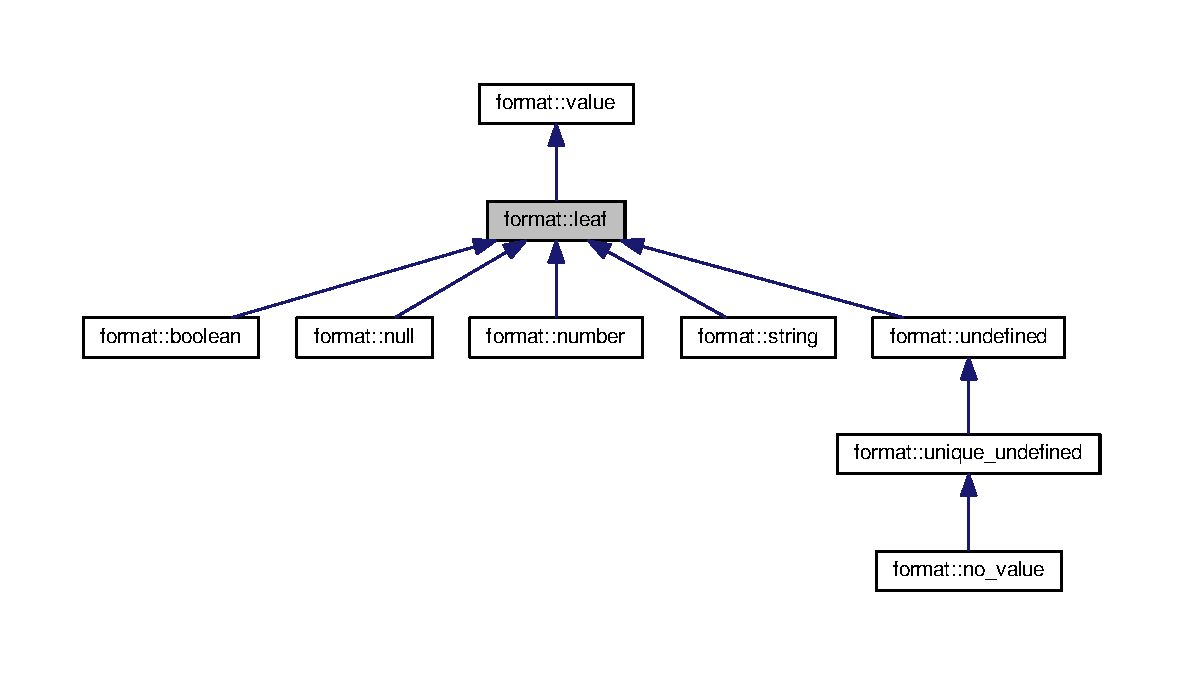
\includegraphics[width=350pt]{classformat_1_1leaf__inherit__graph}
\end{center}
\end{figure}


Collaboration diagram for format\+:\+:leaf\+:
\nopagebreak
\begin{figure}[H]
\begin{center}
\leavevmode
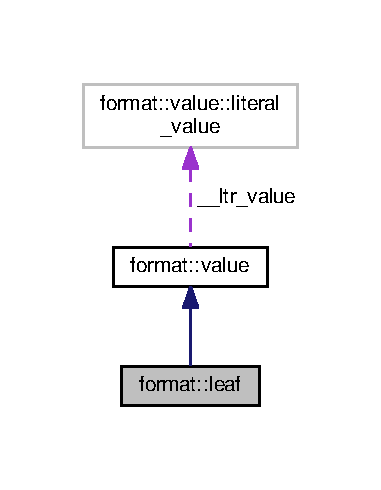
\includegraphics[width=183pt]{classformat_1_1leaf__coll__graph}
\end{center}
\end{figure}
\subsection*{Classes}
\begin{DoxyCompactItemize}
\item 
class \hyperlink{classformat_1_1leaf_1_1iterator}{iterator}
\begin{DoxyCompactList}\small\item\em The iterator class. \end{DoxyCompactList}\end{DoxyCompactItemize}
\subsection*{Public Member Functions}
\begin{DoxyCompactItemize}
\item 
\hyperlink{classformat_1_1leaf_a218f3826712c4cb9056cb61624253d60}{leaf} ()\hypertarget{classformat_1_1leaf_a218f3826712c4cb9056cb61624253d60}{}\label{classformat_1_1leaf_a218f3826712c4cb9056cb61624253d60}

\begin{DoxyCompactList}\small\item\em Leaf. \end{DoxyCompactList}\item 
\hyperlink{classformat_1_1leaf_a21f677a477468cf7604d251d835d0823}{leaf} (const wchar\+\_\+t $\ast$\hyperlink{classformat_1_1json}{json})
\begin{DoxyCompactList}\small\item\em Leaf. \end{DoxyCompactList}\item 
\hyperlink{classformat_1_1leaf_ac3e3d8c7aa7e81bca038b31df80f4aef}{leaf} (\hyperlink{classformat_1_1json}{json} $\ast$\hyperlink{classformat_1_1value_a86c03ec8810bfd0d60ec49095120040d}{parent})
\begin{DoxyCompactList}\small\item\em Leaf. \end{DoxyCompactList}\item 
\hyperlink{classformat_1_1leaf_ac0001e636d8511d4c7bbf59f8cf0706b}{leaf} (const \hyperlink{classformat_1_1leaf}{leaf} \&other)=default
\begin{DoxyCompactList}\small\item\em Leaf. \end{DoxyCompactList}\item 
virtual \hyperlink{classformat_1_1leaf_a445166bd9ca7296bbda80ec4a1128ef1}{$\sim$leaf} () override=default\hypertarget{classformat_1_1leaf_a445166bd9ca7296bbda80ec4a1128ef1}{}\label{classformat_1_1leaf_a445166bd9ca7296bbda80ec4a1128ef1}

\begin{DoxyCompactList}\small\item\em $\sim$\+Leaf \end{DoxyCompactList}\item 
virtual \hyperlink{classformat_1_1value_aa6b85823936bf7b8ab78d3f8d443c00d}{value} $\ast$ \hyperlink{classformat_1_1leaf_a861972c1866ab17d00e4b950d33d4ced}{clone} () const override=0
\begin{DoxyCompactList}\small\item\em \+\_\+clone \end{DoxyCompactList}\item 
virtual \hyperlink{classformat_1_1value_aa0334be06389a7b14af485fa0cd3aa21}{value\+\_\+t} \hyperlink{classformat_1_1leaf_ac29de88719f2da4d262255ef8a234ced}{type} () const noexcept=0
\begin{DoxyCompactList}\small\item\em type \end{DoxyCompactList}\item 
virtual size\+\_\+t \hyperlink{classformat_1_1leaf_ab14acf7466a4a603d4558419d36fe75a}{length} () const noexceptfinaloverride
\begin{DoxyCompactList}\small\item\em size \end{DoxyCompactList}\item 
\hyperlink{classformat_1_1leaf_1_1iterator}{iterator} \hyperlink{classformat_1_1leaf_af4188fcb27d2c56c1b5af0e5db9fc603}{begin} ()
\begin{DoxyCompactList}\small\item\em begin \end{DoxyCompactList}\item 
\hyperlink{classformat_1_1leaf_1_1iterator}{iterator} \hyperlink{classformat_1_1leaf_a95970b9f786076d77448f12c0daa99e2}{end} ()
\begin{DoxyCompactList}\small\item\em end \end{DoxyCompactList}\end{DoxyCompactItemize}
\subsection*{Protected Member Functions}
\begin{DoxyCompactItemize}
\item 
virtual \hyperlink{classformat_1_1value_aa6b85823936bf7b8ab78d3f8d443c00d}{value} \& \hyperlink{classformat_1_1leaf_aa92aad1668dce02132ca0920b8803f1f}{\+\_\+at} (const wchar\+\_\+t $\ast$) finaloverride
\begin{DoxyCompactList}\small\item\em \+\_\+at \end{DoxyCompactList}\item 
virtual \hyperlink{classformat_1_1value_aa6b85823936bf7b8ab78d3f8d443c00d}{value} \& \hyperlink{classformat_1_1leaf_a629bf52297b80f099b6477ff88761a2b}{\+\_\+at} (size\+\_\+t) finaloverride
\begin{DoxyCompactList}\small\item\em \+\_\+at \end{DoxyCompactList}\item 
virtual \hyperlink{classformat_1_1value_aa6b85823936bf7b8ab78d3f8d443c00d}{value} \& \hyperlink{classformat_1_1leaf_ab73b4db4d7aa9d7490bdfb90d31cdc71}{\+\_\+assign} (\hyperlink{classformat_1_1value_aa6b85823936bf7b8ab78d3f8d443c00d}{value} $\ast$, \hyperlink{classformat_1_1value_aa6b85823936bf7b8ab78d3f8d443c00d}{value} $\ast$) finaloverride
\begin{DoxyCompactList}\small\item\em assign \end{DoxyCompactList}\item 
virtual void \hyperlink{classformat_1_1leaf_a98449fdebba18260ac00319e3ad7298f}{\+\_\+clear} ()=0\hypertarget{classformat_1_1leaf_a98449fdebba18260ac00319e3ad7298f}{}\label{classformat_1_1leaf_a98449fdebba18260ac00319e3ad7298f}

\begin{DoxyCompactList}\small\item\em \+\_\+clear \end{DoxyCompactList}\item 
virtual \hyperlink{classformat_1_1value_aa6b85823936bf7b8ab78d3f8d443c00d}{value} \& \hyperlink{classformat_1_1leaf_a666ee6101e4b668aba5925f1c68e2508}{\+\_\+erase} (const \hyperlink{classformat_1_1value_aa6b85823936bf7b8ab78d3f8d443c00d}{value} \&) noexceptfinaloverride
\begin{DoxyCompactList}\small\item\em \+\_\+erase \end{DoxyCompactList}\item 
virtual \hyperlink{classformat_1_1value_aa6b85823936bf7b8ab78d3f8d443c00d}{value} $\ast$ \hyperlink{classformat_1_1leaf_a45f6e4e09027122e445ba3b8352aec14}{\+\_\+clone} (const \hyperlink{classformat_1_1value_aa6b85823936bf7b8ab78d3f8d443c00d}{value} \&)=0
\begin{DoxyCompactList}\small\item\em \+\_\+clone \end{DoxyCompactList}\end{DoxyCompactItemize}
\subsection*{Additional Inherited Members}


\subsection{Detailed Description}
The leaf class. 

\subsection{Constructor \& Destructor Documentation}
\index{format\+::leaf@{format\+::leaf}!leaf@{leaf}}
\index{leaf@{leaf}!format\+::leaf@{format\+::leaf}}
\subsubsection[{\texorpdfstring{leaf(const wchar\+\_\+t $\ast$json)}{leaf(const wchar_t *json)}}]{\setlength{\rightskip}{0pt plus 5cm}format\+::leaf\+::leaf (
\begin{DoxyParamCaption}
\item[{const wchar\+\_\+t $\ast$}]{json}
\end{DoxyParamCaption}
)\hspace{0.3cm}{\ttfamily [inline]}}\hypertarget{classformat_1_1leaf_a21f677a477468cf7604d251d835d0823}{}\label{classformat_1_1leaf_a21f677a477468cf7604d251d835d0823}


Leaf. 


\begin{DoxyParams}{Parameters}
{\em json} & \\
\hline
\end{DoxyParams}
\index{format\+::leaf@{format\+::leaf}!leaf@{leaf}}
\index{leaf@{leaf}!format\+::leaf@{format\+::leaf}}
\subsubsection[{\texorpdfstring{leaf(json $\ast$parent)}{leaf(json *parent)}}]{\setlength{\rightskip}{0pt plus 5cm}format\+::leaf\+::leaf (
\begin{DoxyParamCaption}
\item[{{\bf json} $\ast$}]{parent}
\end{DoxyParamCaption}
)\hspace{0.3cm}{\ttfamily [inline]}}\hypertarget{classformat_1_1leaf_ac3e3d8c7aa7e81bca038b31df80f4aef}{}\label{classformat_1_1leaf_ac3e3d8c7aa7e81bca038b31df80f4aef}


Leaf. 


\begin{DoxyParams}{Parameters}
{\em parent} & \\
\hline
\end{DoxyParams}
\index{format\+::leaf@{format\+::leaf}!leaf@{leaf}}
\index{leaf@{leaf}!format\+::leaf@{format\+::leaf}}
\subsubsection[{\texorpdfstring{leaf(const leaf \&other)=default}{leaf(const leaf &other)=default}}]{\setlength{\rightskip}{0pt plus 5cm}format\+::leaf\+::leaf (
\begin{DoxyParamCaption}
\item[{const {\bf leaf} \&}]{other}
\end{DoxyParamCaption}
)\hspace{0.3cm}{\ttfamily [default]}}\hypertarget{classformat_1_1leaf_ac0001e636d8511d4c7bbf59f8cf0706b}{}\label{classformat_1_1leaf_ac0001e636d8511d4c7bbf59f8cf0706b}


Leaf. 


\begin{DoxyParams}{Parameters}
{\em other} & \\
\hline
\end{DoxyParams}


\subsection{Member Function Documentation}
\index{format\+::leaf@{format\+::leaf}!\+\_\+assign@{\+\_\+assign}}
\index{\+\_\+assign@{\+\_\+assign}!format\+::leaf@{format\+::leaf}}
\subsubsection[{\texorpdfstring{\+\_\+assign(value $\ast$, value $\ast$) finaloverride}{_assign(value *, value *) finaloverride}}]{\setlength{\rightskip}{0pt plus 5cm}virtual {\bf value}\& format\+::leaf\+::\+\_\+assign (
\begin{DoxyParamCaption}
\item[{{\bf value} $\ast$}]{, }
\item[{{\bf value} $\ast$}]{}
\end{DoxyParamCaption}
)\hspace{0.3cm}{\ttfamily [inline]}, {\ttfamily [final]}, {\ttfamily [override]}, {\ttfamily [protected]}, {\ttfamily [virtual]}}\hypertarget{classformat_1_1leaf_ab73b4db4d7aa9d7490bdfb90d31cdc71}{}\label{classformat_1_1leaf_ab73b4db4d7aa9d7490bdfb90d31cdc71}


assign 

\begin{DoxyReturn}{Returns}

\end{DoxyReturn}
\index{format\+::leaf@{format\+::leaf}!\+\_\+at@{\+\_\+at}}
\index{\+\_\+at@{\+\_\+at}!format\+::leaf@{format\+::leaf}}
\subsubsection[{\texorpdfstring{\+\_\+at(const wchar\+\_\+t $\ast$) finaloverride}{_at(const wchar_t *) finaloverride}}]{\setlength{\rightskip}{0pt plus 5cm}virtual {\bf value}\& format\+::leaf\+::\+\_\+at (
\begin{DoxyParamCaption}
\item[{const wchar\+\_\+t $\ast$}]{}
\end{DoxyParamCaption}
)\hspace{0.3cm}{\ttfamily [inline]}, {\ttfamily [final]}, {\ttfamily [override]}, {\ttfamily [protected]}, {\ttfamily [virtual]}}\hypertarget{classformat_1_1leaf_aa92aad1668dce02132ca0920b8803f1f}{}\label{classformat_1_1leaf_aa92aad1668dce02132ca0920b8803f1f}


\+\_\+at 

\begin{DoxyReturn}{Returns}

\end{DoxyReturn}


Implements \hyperlink{classformat_1_1value_a3f67662acb201f2ab8a768f8cb670678}{format\+::value}.

\index{format\+::leaf@{format\+::leaf}!\+\_\+at@{\+\_\+at}}
\index{\+\_\+at@{\+\_\+at}!format\+::leaf@{format\+::leaf}}
\subsubsection[{\texorpdfstring{\+\_\+at(size\+\_\+t) finaloverride}{_at(size_t) finaloverride}}]{\setlength{\rightskip}{0pt plus 5cm}virtual {\bf value}\& format\+::leaf\+::\+\_\+at (
\begin{DoxyParamCaption}
\item[{size\+\_\+t}]{}
\end{DoxyParamCaption}
)\hspace{0.3cm}{\ttfamily [inline]}, {\ttfamily [final]}, {\ttfamily [override]}, {\ttfamily [protected]}, {\ttfamily [virtual]}}\hypertarget{classformat_1_1leaf_a629bf52297b80f099b6477ff88761a2b}{}\label{classformat_1_1leaf_a629bf52297b80f099b6477ff88761a2b}


\+\_\+at 

\begin{DoxyReturn}{Returns}

\end{DoxyReturn}


Implements \hyperlink{classformat_1_1value_ab94a7f0af8ea5c60fd0e59ccde8d0371}{format\+::value}.

\index{format\+::leaf@{format\+::leaf}!\+\_\+clone@{\+\_\+clone}}
\index{\+\_\+clone@{\+\_\+clone}!format\+::leaf@{format\+::leaf}}
\subsubsection[{\texorpdfstring{\+\_\+clone(const value \&)=0}{_clone(const value &)=0}}]{\setlength{\rightskip}{0pt plus 5cm}virtual {\bf value}$\ast$ format\+::leaf\+::\+\_\+clone (
\begin{DoxyParamCaption}
\item[{const {\bf value} \&}]{}
\end{DoxyParamCaption}
)\hspace{0.3cm}{\ttfamily [protected]}, {\ttfamily [pure virtual]}}\hypertarget{classformat_1_1leaf_a45f6e4e09027122e445ba3b8352aec14}{}\label{classformat_1_1leaf_a45f6e4e09027122e445ba3b8352aec14}


\+\_\+clone 

\begin{DoxyReturn}{Returns}

\end{DoxyReturn}


Implemented in \hyperlink{classformat_1_1number_a995497a87887619195ebb4f96e7faa88}{format\+::number}, \hyperlink{classformat_1_1undefined_aacb01d587e4e623a450e5e477d25bf71}{format\+::undefined}, \hyperlink{classformat_1_1boolean_aa736f994233dad5fa8fcef030e50e2d7}{format\+::boolean}, \hyperlink{classformat_1_1string_a876061b10e5edf4d8ba9801bf819f8c9}{format\+::string}, and \hyperlink{classformat_1_1null_ae43d32571c3b127c43ac4f588cfa9b6a}{format\+::null}.

\index{format\+::leaf@{format\+::leaf}!\+\_\+erase@{\+\_\+erase}}
\index{\+\_\+erase@{\+\_\+erase}!format\+::leaf@{format\+::leaf}}
\subsubsection[{\texorpdfstring{\+\_\+erase(const value \&) noexceptfinaloverride}{_erase(const value &) noexceptfinaloverride}}]{\setlength{\rightskip}{0pt plus 5cm}virtual {\bf value}\& format\+::leaf\+::\+\_\+erase (
\begin{DoxyParamCaption}
\item[{const {\bf value} \&}]{}
\end{DoxyParamCaption}
)\hspace{0.3cm}{\ttfamily [inline]}, {\ttfamily [final]}, {\ttfamily [override]}, {\ttfamily [protected]}, {\ttfamily [virtual]}, {\ttfamily [noexcept]}}\hypertarget{classformat_1_1leaf_a666ee6101e4b668aba5925f1c68e2508}{}\label{classformat_1_1leaf_a666ee6101e4b668aba5925f1c68e2508}


\+\_\+erase 

\begin{DoxyReturn}{Returns}

\end{DoxyReturn}
\index{format\+::leaf@{format\+::leaf}!begin@{begin}}
\index{begin@{begin}!format\+::leaf@{format\+::leaf}}
\subsubsection[{\texorpdfstring{begin()}{begin()}}]{\setlength{\rightskip}{0pt plus 5cm}{\bf iterator} format\+::leaf\+::begin (
\begin{DoxyParamCaption}
{}
\end{DoxyParamCaption}
)\hspace{0.3cm}{\ttfamily [inline]}}\hypertarget{classformat_1_1leaf_af4188fcb27d2c56c1b5af0e5db9fc603}{}\label{classformat_1_1leaf_af4188fcb27d2c56c1b5af0e5db9fc603}


begin 

\begin{DoxyReturn}{Returns}

\end{DoxyReturn}
\index{format\+::leaf@{format\+::leaf}!clone@{clone}}
\index{clone@{clone}!format\+::leaf@{format\+::leaf}}
\subsubsection[{\texorpdfstring{clone() const override=0}{clone() const override=0}}]{\setlength{\rightskip}{0pt plus 5cm}virtual {\bf value}$\ast$ format\+::leaf\+::clone (
\begin{DoxyParamCaption}
{}
\end{DoxyParamCaption}
) const\hspace{0.3cm}{\ttfamily [override]}, {\ttfamily [pure virtual]}}\hypertarget{classformat_1_1leaf_a861972c1866ab17d00e4b950d33d4ced}{}\label{classformat_1_1leaf_a861972c1866ab17d00e4b950d33d4ced}


\+\_\+clone 

\begin{DoxyReturn}{Returns}

\end{DoxyReturn}


Implements \hyperlink{classformat_1_1value_a8756eb79e41851859d83ae46069dc400}{format\+::value}.



Implemented in \hyperlink{classformat_1_1unique__undefined_af69057a00374c21c5cd73dc77efffb0e}{format\+::unique\+\_\+undefined}, \hyperlink{classformat_1_1undefined_af418bdce70e2d41131ac640fcf6dc121}{format\+::undefined}, \hyperlink{classformat_1_1number_aa4c1aec4e42a504ea16f6b09c2223d9e}{format\+::number}, \hyperlink{classformat_1_1boolean_aed9485ecc21695be4ef8f03cd1034b1e}{format\+::boolean}, \hyperlink{classformat_1_1string_a41b0ffc3e1c686bc07fbe911942a0a4f}{format\+::string}, and \hyperlink{classformat_1_1null_a5a36484f97cd8795e42981f8c30181c2}{format\+::null}.

\index{format\+::leaf@{format\+::leaf}!end@{end}}
\index{end@{end}!format\+::leaf@{format\+::leaf}}
\subsubsection[{\texorpdfstring{end()}{end()}}]{\setlength{\rightskip}{0pt plus 5cm}{\bf iterator} format\+::leaf\+::end (
\begin{DoxyParamCaption}
{}
\end{DoxyParamCaption}
)\hspace{0.3cm}{\ttfamily [inline]}}\hypertarget{classformat_1_1leaf_a95970b9f786076d77448f12c0daa99e2}{}\label{classformat_1_1leaf_a95970b9f786076d77448f12c0daa99e2}


end 

\begin{DoxyReturn}{Returns}

\end{DoxyReturn}
\index{format\+::leaf@{format\+::leaf}!length@{length}}
\index{length@{length}!format\+::leaf@{format\+::leaf}}
\subsubsection[{\texorpdfstring{length() const noexceptfinaloverride}{length() const noexceptfinaloverride}}]{\setlength{\rightskip}{0pt plus 5cm}virtual size\+\_\+t format\+::leaf\+::length (
\begin{DoxyParamCaption}
{}
\end{DoxyParamCaption}
) const\hspace{0.3cm}{\ttfamily [inline]}, {\ttfamily [final]}, {\ttfamily [override]}, {\ttfamily [virtual]}, {\ttfamily [noexcept]}}\hypertarget{classformat_1_1leaf_ab14acf7466a4a603d4558419d36fe75a}{}\label{classformat_1_1leaf_ab14acf7466a4a603d4558419d36fe75a}


size 

\begin{DoxyReturn}{Returns}

\end{DoxyReturn}


Implements \hyperlink{classformat_1_1value_a406a9553c4d83a0613aa54d77f6c462d}{format\+::value}.

\index{format\+::leaf@{format\+::leaf}!type@{type}}
\index{type@{type}!format\+::leaf@{format\+::leaf}}
\subsubsection[{\texorpdfstring{type() const noexcept=0}{type() const noexcept=0}}]{\setlength{\rightskip}{0pt plus 5cm}virtual {\bf value\+\_\+t} format\+::leaf\+::type (
\begin{DoxyParamCaption}
{}
\end{DoxyParamCaption}
) const\hspace{0.3cm}{\ttfamily [pure virtual]}, {\ttfamily [noexcept]}}\hypertarget{classformat_1_1leaf_ac29de88719f2da4d262255ef8a234ced}{}\label{classformat_1_1leaf_ac29de88719f2da4d262255ef8a234ced}


type 

\begin{DoxyReturn}{Returns}

\end{DoxyReturn}


Implements \hyperlink{classformat_1_1value_a7112d0f83cf61aa9e1cdde90fc444996}{format\+::value}.



Implemented in \hyperlink{classformat_1_1no__value_a2819b3ce13265c40a74d4f11c2577bf5}{format\+::no\+\_\+value}, \hyperlink{classformat_1_1undefined_a72e4ff819514b2a4126be1969d5bbabe}{format\+::undefined}, \hyperlink{classformat_1_1number_a1934b4d3cf603de3afd5eb6329be7fba}{format\+::number}, \hyperlink{classformat_1_1boolean_a91dccd7986764af76b70627a348f27a4}{format\+::boolean}, \hyperlink{classformat_1_1null_a3878d16875e190e0f319bf6f600883c9}{format\+::null}, and \hyperlink{classformat_1_1string_a247e17aaf8cb8e0afdc29e943d492232}{format\+::string}.



The documentation for this class was generated from the following file\+:\begin{DoxyCompactItemize}
\item 
json\+\_\+leaf.\+h\end{DoxyCompactItemize}

\hypertarget{classformat_1_1no__value}{}\section{format\+:\+:no\+\_\+value Class Reference}
\label{classformat_1_1no__value}\index{format\+::no\+\_\+value@{format\+::no\+\_\+value}}


The \hyperlink{classformat_1_1no__value}{no\+\_\+value} class.  




{\ttfamily \#include $<$json\+\_\+undefined.\+h$>$}



Inheritance diagram for format\+:\+:no\+\_\+value\+:
\nopagebreak
\begin{figure}[H]
\begin{center}
\leavevmode
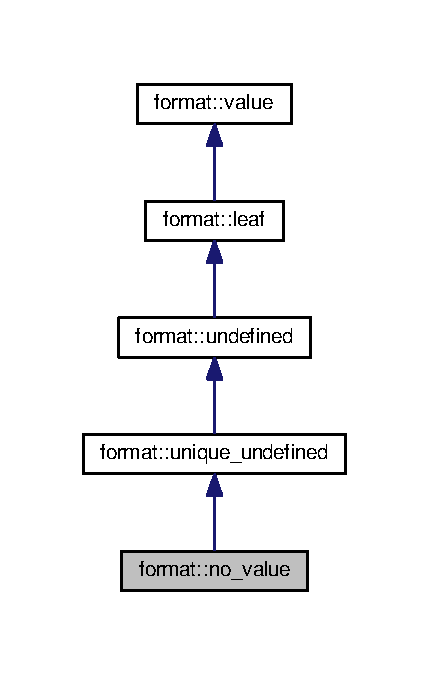
\includegraphics[width=206pt]{classformat_1_1no__value__inherit__graph}
\end{center}
\end{figure}


Collaboration diagram for format\+:\+:no\+\_\+value\+:
\nopagebreak
\begin{figure}[H]
\begin{center}
\leavevmode
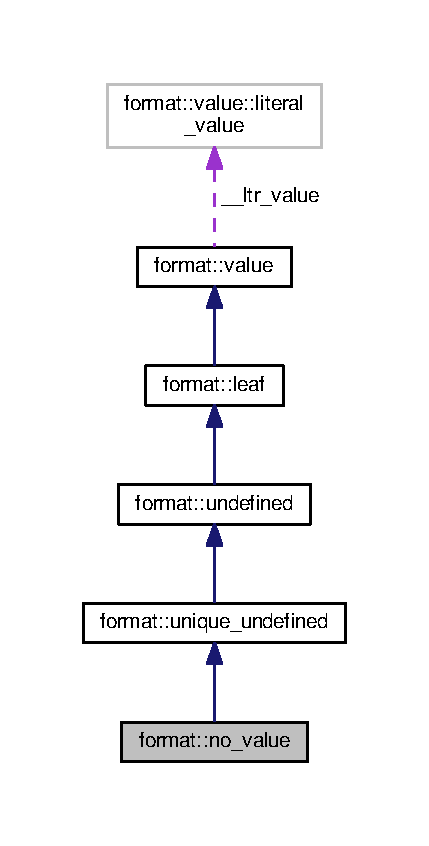
\includegraphics[width=206pt]{classformat_1_1no__value__coll__graph}
\end{center}
\end{figure}
\subsection*{Public Member Functions}
\begin{DoxyCompactItemize}
\item 
void {\bfseries operator delete} (void $\ast$)\hypertarget{classformat_1_1no__value_a0e3cf7fff86241a7ca840a5ab6aa0097}{}\label{classformat_1_1no__value_a0e3cf7fff86241a7ca840a5ab6aa0097}

\item 
void {\bfseries operator delete\mbox{[}$\,$\mbox{]}} (void $\ast$)\hypertarget{classformat_1_1no__value_a8a81fb06723992b2daa275deffd23517}{}\label{classformat_1_1no__value_a8a81fb06723992b2daa275deffd23517}

\item 
virtual \hyperlink{classformat_1_1no__value_a86937bee6e9e4d514d33070be05ad7c6}{$\sim$no\+\_\+value} () override=default\hypertarget{classformat_1_1no__value_a86937bee6e9e4d514d33070be05ad7c6}{}\label{classformat_1_1no__value_a86937bee6e9e4d514d33070be05ad7c6}

\begin{DoxyCompactList}\small\item\em $\sim$no\+\_\+value \end{DoxyCompactList}\item 
virtual \hyperlink{classformat_1_1value_aa0334be06389a7b14af485fa0cd3aa21}{value\+\_\+t} \hyperlink{classformat_1_1no__value_a2819b3ce13265c40a74d4f11c2577bf5}{type} () const noexceptoverride
\begin{DoxyCompactList}\small\item\em type \end{DoxyCompactList}\end{DoxyCompactItemize}
\subsection*{Static Public Member Functions}
\begin{DoxyCompactItemize}
\item 
static \hyperlink{classformat_1_1no__value}{no\+\_\+value} $\ast$ \hyperlink{classformat_1_1no__value_aba9972bb8f7336f2f62270ceee861abf}{instance} (\hyperlink{classformat_1_1json}{json} $\ast$\hyperlink{classformat_1_1value_a86c03ec8810bfd0d60ec49095120040d}{parent})
\begin{DoxyCompactList}\small\item\em instance \end{DoxyCompactList}\end{DoxyCompactItemize}
\subsection*{Protected Member Functions}
\begin{DoxyCompactItemize}
\item 
\hyperlink{classformat_1_1no__value_a454edf863f43cfdd453687c74418e8c0}{no\+\_\+value} (\hyperlink{classformat_1_1json}{json} $\ast$\hyperlink{classformat_1_1value_a86c03ec8810bfd0d60ec49095120040d}{parent})\hypertarget{classformat_1_1no__value_a454edf863f43cfdd453687c74418e8c0}{}\label{classformat_1_1no__value_a454edf863f43cfdd453687c74418e8c0}

\begin{DoxyCompactList}\small\item\em No\+\_\+\+Value. \end{DoxyCompactList}\end{DoxyCompactItemize}
\subsection*{Additional Inherited Members}


\subsection{Detailed Description}
The \hyperlink{classformat_1_1no__value}{no\+\_\+value} class. 

\subsection{Member Function Documentation}
\index{format\+::no\+\_\+value@{format\+::no\+\_\+value}!instance@{instance}}
\index{instance@{instance}!format\+::no\+\_\+value@{format\+::no\+\_\+value}}
\subsubsection[{\texorpdfstring{instance(json $\ast$parent)}{instance(json *parent)}}]{\setlength{\rightskip}{0pt plus 5cm}{\bf format\+::no\+\_\+value} $\ast$ format\+::no\+\_\+value\+::instance (
\begin{DoxyParamCaption}
\item[{{\bf json} $\ast$}]{parent}
\end{DoxyParamCaption}
)\hspace{0.3cm}{\ttfamily [static]}}\hypertarget{classformat_1_1no__value_aba9972bb8f7336f2f62270ceee861abf}{}\label{classformat_1_1no__value_aba9972bb8f7336f2f62270ceee861abf}


instance 


\begin{DoxyParams}{Parameters}
{\em parent} & \\
\hline
\end{DoxyParams}
\begin{DoxyReturn}{Returns}

\end{DoxyReturn}
\index{format\+::no\+\_\+value@{format\+::no\+\_\+value}!type@{type}}
\index{type@{type}!format\+::no\+\_\+value@{format\+::no\+\_\+value}}
\subsubsection[{\texorpdfstring{type() const noexceptoverride}{type() const noexceptoverride}}]{\setlength{\rightskip}{0pt plus 5cm}virtual {\bf value\+\_\+t} format\+::no\+\_\+value\+::type (
\begin{DoxyParamCaption}
{}
\end{DoxyParamCaption}
) const\hspace{0.3cm}{\ttfamily [inline]}, {\ttfamily [override]}, {\ttfamily [virtual]}, {\ttfamily [noexcept]}}\hypertarget{classformat_1_1no__value_a2819b3ce13265c40a74d4f11c2577bf5}{}\label{classformat_1_1no__value_a2819b3ce13265c40a74d4f11c2577bf5}


type 

\begin{DoxyReturn}{Returns}

\end{DoxyReturn}


Reimplemented from \hyperlink{classformat_1_1undefined_a72e4ff819514b2a4126be1969d5bbabe}{format\+::undefined}.



The documentation for this class was generated from the following files\+:\begin{DoxyCompactItemize}
\item 
json\+\_\+undefined.\+h\item 
json\+\_\+undefined.\+cpp\end{DoxyCompactItemize}

\hypertarget{classformat_1_1null}{}\section{format\+:\+:null Class Reference}
\label{classformat_1_1null}\index{format\+::null@{format\+::null}}


The null class.  




{\ttfamily \#include $<$json\+\_\+null.\+h$>$}



Inheritance diagram for format\+:\+:null\+:
\nopagebreak
\begin{figure}[H]
\begin{center}
\leavevmode
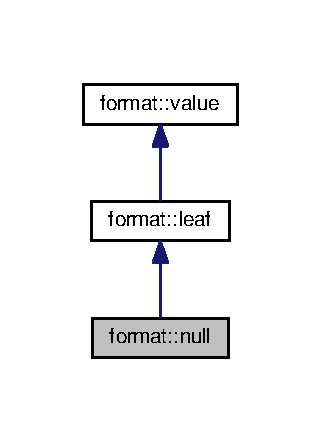
\includegraphics[width=154pt]{classformat_1_1null__inherit__graph}
\end{center}
\end{figure}


Collaboration diagram for format\+:\+:null\+:
\nopagebreak
\begin{figure}[H]
\begin{center}
\leavevmode
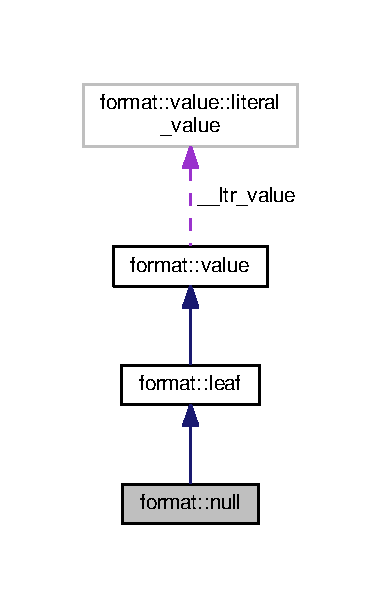
\includegraphics[width=183pt]{classformat_1_1null__coll__graph}
\end{center}
\end{figure}
\subsection*{Public Member Functions}
\begin{DoxyCompactItemize}
\item 
\hyperlink{classformat_1_1null_ad9f30cebcd6641b4a4a57df7ae069851}{null} ()\hypertarget{classformat_1_1null_ad9f30cebcd6641b4a4a57df7ae069851}{}\label{classformat_1_1null_ad9f30cebcd6641b4a4a57df7ae069851}

\begin{DoxyCompactList}\small\item\em null \end{DoxyCompactList}\item 
\hyperlink{classformat_1_1null_ad406608e47f7aa9975992f23b99bd996}{null} (const \hyperlink{classformat_1_1null}{null} \&other)=default
\begin{DoxyCompactList}\small\item\em Null. \end{DoxyCompactList}\item 
virtual \hyperlink{classformat_1_1null_a4d04350101ca2371ad0063467182f5a1}{$\sim$null} () override=default\hypertarget{classformat_1_1null_a4d04350101ca2371ad0063467182f5a1}{}\label{classformat_1_1null_a4d04350101ca2371ad0063467182f5a1}

\begin{DoxyCompactList}\small\item\em $\sim$null \end{DoxyCompactList}\item 
virtual \hyperlink{classformat_1_1value_aa6b85823936bf7b8ab78d3f8d443c00d}{value} $\ast$ \hyperlink{classformat_1_1null_a5a36484f97cd8795e42981f8c30181c2}{clone} () const 
\begin{DoxyCompactList}\small\item\em clone \end{DoxyCompactList}\item 
virtual const wchar\+\_\+t $\ast$ \hyperlink{classformat_1_1null_a7cb0c2e0582c244746f2dafb8712e19a}{\+\_\+parse} (const wchar\+\_\+t $\ast$\hyperlink{classformat_1_1json}{json}) override
\begin{DoxyCompactList}\small\item\em \+\_\+parse \end{DoxyCompactList}\item 
virtual \hyperlink{classformat_1_1value_aa0334be06389a7b14af485fa0cd3aa21}{value\+::value\+\_\+t} \hyperlink{classformat_1_1null_a3878d16875e190e0f319bf6f600883c9}{type} () const noexceptoverride
\begin{DoxyCompactList}\small\item\em type \end{DoxyCompactList}\item 
std\+::nullptr\+\_\+t \hyperlink{classformat_1_1null_ae32163fe796ecb28e12afcbc6fa47ea4}{get} () const noexcept
\begin{DoxyCompactList}\small\item\em Value. \end{DoxyCompactList}\item 
\hyperlink{classformat_1_1value_aa6b85823936bf7b8ab78d3f8d443c00d}{value} \& \hyperlink{classformat_1_1null_a0d04f44f36c54d8192ac40aeb5540f41}{operator=} (const \hyperlink{classformat_1_1null}{null} \&n)
\begin{DoxyCompactList}\small\item\em operator = \end{DoxyCompactList}\item 
virtual size\+\_\+t \hyperlink{classformat_1_1null_ae5df2937bf5677e5894685ff47654642}{str\+\_\+length} () const noexceptoverride
\begin{DoxyCompactList}\small\item\em str\+Length \end{DoxyCompactList}\end{DoxyCompactItemize}
\subsection*{Protected Member Functions}
\begin{DoxyCompactItemize}
\item 
\hyperlink{classformat_1_1null_aeaec053f34742b73ceee29fa52c89a07}{null} (\hyperlink{classformat_1_1json}{json} $\ast$\hyperlink{classformat_1_1value_a86c03ec8810bfd0d60ec49095120040d}{parent})
\begin{DoxyCompactList}\small\item\em null \end{DoxyCompactList}\item 
\hyperlink{classformat_1_1value_aa6b85823936bf7b8ab78d3f8d443c00d}{value} \& \hyperlink{classformat_1_1null_a78e3069d06d7d7b96601119e4c940013}{\+\_\+assign} (const \hyperlink{classformat_1_1null}{null} \&)
\begin{DoxyCompactList}\small\item\em assign \end{DoxyCompactList}\item 
virtual void \hyperlink{classformat_1_1null_a0ee1ca6d5fa2957d7000e8673b6c4168}{\+\_\+clear} ()\hypertarget{classformat_1_1null_a0ee1ca6d5fa2957d7000e8673b6c4168}{}\label{classformat_1_1null_a0ee1ca6d5fa2957d7000e8673b6c4168}

\begin{DoxyCompactList}\small\item\em \+\_\+clear \end{DoxyCompactList}\item 
virtual \hyperlink{classformat_1_1value_aa6b85823936bf7b8ab78d3f8d443c00d}{value} $\ast$ \hyperlink{classformat_1_1null_ae43d32571c3b127c43ac4f588cfa9b6a}{\+\_\+clone} (const \hyperlink{classformat_1_1value_aa6b85823936bf7b8ab78d3f8d443c00d}{value} \&) override
\begin{DoxyCompactList}\small\item\em \+\_\+clone \end{DoxyCompactList}\item 
virtual const wchar\+\_\+t $\ast$ \hyperlink{classformat_1_1null_a8c85176815e031702c5487573b07ffac}{\+\_\+to\+\_\+string} (wchar\+\_\+t $\ast$) const noexceptoverride
\begin{DoxyCompactList}\small\item\em str\+Value \end{DoxyCompactList}\end{DoxyCompactItemize}
\subsection*{Friends}
\begin{DoxyCompactItemize}
\item 
\hyperlink{classformat_1_1null}{null} $\ast$ {\bfseries \+\_\+\+\_\+call\+\_\+null} (\hyperlink{classformat_1_1json}{json} $\ast$)\hypertarget{classformat_1_1null_accd6c2901e09fe6015df1ef58e3f1fcb}{}\label{classformat_1_1null_accd6c2901e09fe6015df1ef58e3f1fcb}

\end{DoxyCompactItemize}
\subsection*{Additional Inherited Members}


\subsection{Detailed Description}
The null class. 

\subsection{Constructor \& Destructor Documentation}
\index{format\+::null@{format\+::null}!null@{null}}
\index{null@{null}!format\+::null@{format\+::null}}
\subsubsection[{\texorpdfstring{null(const null \&other)=default}{null(const null &other)=default}}]{\setlength{\rightskip}{0pt plus 5cm}format\+::null\+::null (
\begin{DoxyParamCaption}
\item[{const {\bf null} \&}]{other}
\end{DoxyParamCaption}
)\hspace{0.3cm}{\ttfamily [default]}}\hypertarget{classformat_1_1null_ad406608e47f7aa9975992f23b99bd996}{}\label{classformat_1_1null_ad406608e47f7aa9975992f23b99bd996}


Null. 


\begin{DoxyParams}{Parameters}
{\em other} & \\
\hline
\end{DoxyParams}
\index{format\+::null@{format\+::null}!null@{null}}
\index{null@{null}!format\+::null@{format\+::null}}
\subsubsection[{\texorpdfstring{null(json $\ast$parent)}{null(json *parent)}}]{\setlength{\rightskip}{0pt plus 5cm}format\+::null\+::null (
\begin{DoxyParamCaption}
\item[{{\bf json} $\ast$}]{parent}
\end{DoxyParamCaption}
)\hspace{0.3cm}{\ttfamily [inline]}, {\ttfamily [protected]}}\hypertarget{classformat_1_1null_aeaec053f34742b73ceee29fa52c89a07}{}\label{classformat_1_1null_aeaec053f34742b73ceee29fa52c89a07}


null 


\begin{DoxyParams}{Parameters}
{\em parent} & \\
\hline
\end{DoxyParams}


\subsection{Member Function Documentation}
\index{format\+::null@{format\+::null}!\+\_\+assign@{\+\_\+assign}}
\index{\+\_\+assign@{\+\_\+assign}!format\+::null@{format\+::null}}
\subsubsection[{\texorpdfstring{\+\_\+assign(const null \&)}{_assign(const null &)}}]{\setlength{\rightskip}{0pt plus 5cm}{\bf value}\& format\+::null\+::\+\_\+assign (
\begin{DoxyParamCaption}
\item[{const {\bf null} \&}]{}
\end{DoxyParamCaption}
)\hspace{0.3cm}{\ttfamily [inline]}, {\ttfamily [protected]}}\hypertarget{classformat_1_1null_a78e3069d06d7d7b96601119e4c940013}{}\label{classformat_1_1null_a78e3069d06d7d7b96601119e4c940013}


assign 


\begin{DoxyParams}{Parameters}
{\em nv} & \\
\hline
\end{DoxyParams}
\begin{DoxyReturn}{Returns}

\end{DoxyReturn}
\index{format\+::null@{format\+::null}!\+\_\+clone@{\+\_\+clone}}
\index{\+\_\+clone@{\+\_\+clone}!format\+::null@{format\+::null}}
\subsubsection[{\texorpdfstring{\+\_\+clone(const value \&) override}{_clone(const value &) override}}]{\setlength{\rightskip}{0pt plus 5cm}virtual {\bf value}$\ast$ format\+::null\+::\+\_\+clone (
\begin{DoxyParamCaption}
\item[{const {\bf value} \&}]{}
\end{DoxyParamCaption}
)\hspace{0.3cm}{\ttfamily [inline]}, {\ttfamily [override]}, {\ttfamily [protected]}, {\ttfamily [virtual]}}\hypertarget{classformat_1_1null_ae43d32571c3b127c43ac4f588cfa9b6a}{}\label{classformat_1_1null_ae43d32571c3b127c43ac4f588cfa9b6a}


\+\_\+clone 

\begin{DoxyReturn}{Returns}

\end{DoxyReturn}


Implements \hyperlink{classformat_1_1leaf_a45f6e4e09027122e445ba3b8352aec14}{format\+::leaf}.

\index{format\+::null@{format\+::null}!\+\_\+parse@{\+\_\+parse}}
\index{\+\_\+parse@{\+\_\+parse}!format\+::null@{format\+::null}}
\subsubsection[{\texorpdfstring{\+\_\+parse(const wchar\+\_\+t $\ast$json) override}{_parse(const wchar_t *json) override}}]{\setlength{\rightskip}{0pt plus 5cm}virtual const wchar\+\_\+t$\ast$ format\+::null\+::\+\_\+parse (
\begin{DoxyParamCaption}
\item[{const wchar\+\_\+t $\ast$}]{json}
\end{DoxyParamCaption}
)\hspace{0.3cm}{\ttfamily [inline]}, {\ttfamily [override]}, {\ttfamily [virtual]}}\hypertarget{classformat_1_1null_a7cb0c2e0582c244746f2dafb8712e19a}{}\label{classformat_1_1null_a7cb0c2e0582c244746f2dafb8712e19a}


\+\_\+parse 


\begin{DoxyParams}{Parameters}
{\em json} & \\
\hline
\end{DoxyParams}
\begin{DoxyReturn}{Returns}

\end{DoxyReturn}


Implements \hyperlink{classformat_1_1value_a7859b1aa48f667a83e091f0eba22d4a1}{format\+::value}.

\index{format\+::null@{format\+::null}!\+\_\+to\+\_\+string@{\+\_\+to\+\_\+string}}
\index{\+\_\+to\+\_\+string@{\+\_\+to\+\_\+string}!format\+::null@{format\+::null}}
\subsubsection[{\texorpdfstring{\+\_\+to\+\_\+string(wchar\+\_\+t $\ast$) const noexceptoverride}{_to_string(wchar_t *) const noexceptoverride}}]{\setlength{\rightskip}{0pt plus 5cm}virtual const wchar\+\_\+t$\ast$ format\+::null\+::\+\_\+to\+\_\+string (
\begin{DoxyParamCaption}
\item[{wchar\+\_\+t $\ast$}]{}
\end{DoxyParamCaption}
) const\hspace{0.3cm}{\ttfamily [inline]}, {\ttfamily [override]}, {\ttfamily [protected]}, {\ttfamily [virtual]}, {\ttfamily [noexcept]}}\hypertarget{classformat_1_1null_a8c85176815e031702c5487573b07ffac}{}\label{classformat_1_1null_a8c85176815e031702c5487573b07ffac}


str\+Value 

\begin{DoxyReturn}{Returns}

\end{DoxyReturn}


Implements \hyperlink{classformat_1_1value_a94ed31f07b19866495297472accd33a8}{format\+::value}.

\index{format\+::null@{format\+::null}!clone@{clone}}
\index{clone@{clone}!format\+::null@{format\+::null}}
\subsubsection[{\texorpdfstring{clone() const }{clone() const }}]{\setlength{\rightskip}{0pt plus 5cm}virtual {\bf value}$\ast$ format\+::null\+::clone (
\begin{DoxyParamCaption}
{}
\end{DoxyParamCaption}
) const\hspace{0.3cm}{\ttfamily [inline]}, {\ttfamily [virtual]}}\hypertarget{classformat_1_1null_a5a36484f97cd8795e42981f8c30181c2}{}\label{classformat_1_1null_a5a36484f97cd8795e42981f8c30181c2}


clone 


\begin{DoxyParams}{Parameters}
{\em other} & \\
\hline
\end{DoxyParams}
\begin{DoxyReturn}{Returns}

\end{DoxyReturn}


Implements \hyperlink{classformat_1_1leaf_a861972c1866ab17d00e4b950d33d4ced}{format\+::leaf}.

\index{format\+::null@{format\+::null}!get@{get}}
\index{get@{get}!format\+::null@{format\+::null}}
\subsubsection[{\texorpdfstring{get() const noexcept}{get() const noexcept}}]{\setlength{\rightskip}{0pt plus 5cm}std\+::nullptr\+\_\+t format\+::null\+::get (
\begin{DoxyParamCaption}
{}
\end{DoxyParamCaption}
) const\hspace{0.3cm}{\ttfamily [inline]}, {\ttfamily [noexcept]}}\hypertarget{classformat_1_1null_ae32163fe796ecb28e12afcbc6fa47ea4}{}\label{classformat_1_1null_ae32163fe796ecb28e12afcbc6fa47ea4}


Value. 

\begin{DoxyReturn}{Returns}

\end{DoxyReturn}
\index{format\+::null@{format\+::null}!operator=@{operator=}}
\index{operator=@{operator=}!format\+::null@{format\+::null}}
\subsubsection[{\texorpdfstring{operator=(const null \&n)}{operator=(const null &n)}}]{\setlength{\rightskip}{0pt plus 5cm}{\bf value}\& format\+::null\+::operator= (
\begin{DoxyParamCaption}
\item[{const {\bf null} \&}]{n}
\end{DoxyParamCaption}
)\hspace{0.3cm}{\ttfamily [inline]}}\hypertarget{classformat_1_1null_a0d04f44f36c54d8192ac40aeb5540f41}{}\label{classformat_1_1null_a0d04f44f36c54d8192ac40aeb5540f41}


operator = 


\begin{DoxyParams}{Parameters}
{\em n} & \\
\hline
\end{DoxyParams}
\begin{DoxyReturn}{Returns}

\end{DoxyReturn}
\index{format\+::null@{format\+::null}!str\+\_\+length@{str\+\_\+length}}
\index{str\+\_\+length@{str\+\_\+length}!format\+::null@{format\+::null}}
\subsubsection[{\texorpdfstring{str\+\_\+length() const noexceptoverride}{str_length() const noexceptoverride}}]{\setlength{\rightskip}{0pt plus 5cm}virtual size\+\_\+t format\+::null\+::str\+\_\+length (
\begin{DoxyParamCaption}
{}
\end{DoxyParamCaption}
) const\hspace{0.3cm}{\ttfamily [inline]}, {\ttfamily [override]}, {\ttfamily [virtual]}, {\ttfamily [noexcept]}}\hypertarget{classformat_1_1null_ae5df2937bf5677e5894685ff47654642}{}\label{classformat_1_1null_ae5df2937bf5677e5894685ff47654642}


str\+Length 

\begin{DoxyReturn}{Returns}

\end{DoxyReturn}


Implements \hyperlink{classformat_1_1value_a399280e27e629db0582b5781b90ca58b}{format\+::value}.

\index{format\+::null@{format\+::null}!type@{type}}
\index{type@{type}!format\+::null@{format\+::null}}
\subsubsection[{\texorpdfstring{type() const noexceptoverride}{type() const noexceptoverride}}]{\setlength{\rightskip}{0pt plus 5cm}virtual {\bf value\+::value\+\_\+t} format\+::null\+::type (
\begin{DoxyParamCaption}
{}
\end{DoxyParamCaption}
) const\hspace{0.3cm}{\ttfamily [inline]}, {\ttfamily [override]}, {\ttfamily [virtual]}, {\ttfamily [noexcept]}}\hypertarget{classformat_1_1null_a3878d16875e190e0f319bf6f600883c9}{}\label{classformat_1_1null_a3878d16875e190e0f319bf6f600883c9}


type 

\begin{DoxyReturn}{Returns}

\end{DoxyReturn}


Implements \hyperlink{classformat_1_1leaf_ac29de88719f2da4d262255ef8a234ced}{format\+::leaf}.



The documentation for this class was generated from the following file\+:\begin{DoxyCompactItemize}
\item 
json\+\_\+null.\+h\end{DoxyCompactItemize}

\hypertarget{classformat_1_1number}{}\section{format\+:\+:number Class Reference}
\label{classformat_1_1number}\index{format\+::number@{format\+::number}}


The number class.  




{\ttfamily \#include $<$json\+\_\+number.\+h$>$}



Inheritance diagram for format\+:\+:number\+:
\nopagebreak
\begin{figure}[H]
\begin{center}
\leavevmode
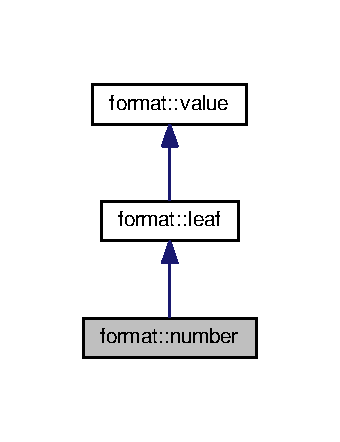
\includegraphics[width=163pt]{classformat_1_1number__inherit__graph}
\end{center}
\end{figure}


Collaboration diagram for format\+:\+:number\+:
\nopagebreak
\begin{figure}[H]
\begin{center}
\leavevmode
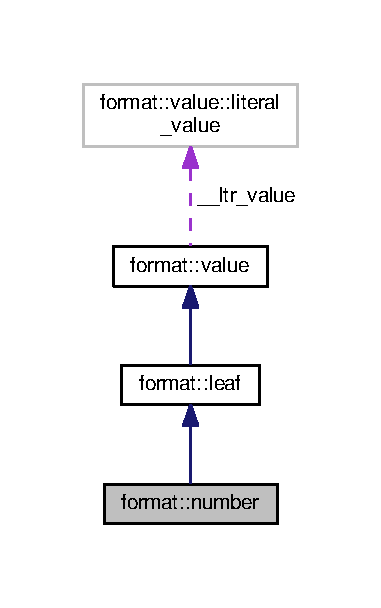
\includegraphics[width=183pt]{classformat_1_1number__coll__graph}
\end{center}
\end{figure}
\subsection*{Public Member Functions}
\begin{DoxyCompactItemize}
\item 
\hyperlink{classformat_1_1number_a58066aeca6b6d93482c0f90038fa3b32}{number} ()\hypertarget{classformat_1_1number_a58066aeca6b6d93482c0f90038fa3b32}{}\label{classformat_1_1number_a58066aeca6b6d93482c0f90038fa3b32}

\begin{DoxyCompactList}\small\item\em Number. \end{DoxyCompactList}\item 
\hyperlink{classformat_1_1number_acea9b475fe9ad85524c63871b9883fa0}{number} (double d)
\begin{DoxyCompactList}\small\item\em number \end{DoxyCompactList}\item 
\hyperlink{classformat_1_1number_a8b5dc6dac86b17a82614ffa9f7aa4791}{number} (const wchar\+\_\+t $\ast$\hyperlink{classformat_1_1json}{json})
\begin{DoxyCompactList}\small\item\em Number. \end{DoxyCompactList}\item 
\hyperlink{classformat_1_1number_a564ebd8714e06cec52daa5c62dbb37b1}{number} (const \hyperlink{classformat_1_1number}{number} \&other)
\begin{DoxyCompactList}\small\item\em Number. \end{DoxyCompactList}\item 
virtual \hyperlink{classformat_1_1number_ab9112b9c312f94488ba48187779787c9}{$\sim$number} () override=default
\begin{DoxyCompactList}\small\item\em $\sim$number \end{DoxyCompactList}\item 
virtual \hyperlink{classformat_1_1value_aa6b85823936bf7b8ab78d3f8d443c00d}{value} $\ast$ \hyperlink{classformat_1_1number_aa4c1aec4e42a504ea16f6b09c2223d9e}{clone} () const 
\begin{DoxyCompactList}\small\item\em clone \end{DoxyCompactList}\item 
virtual \hyperlink{classformat_1_1value_aa0334be06389a7b14af485fa0cd3aa21}{value\+\_\+t} \hyperlink{classformat_1_1number_a1934b4d3cf603de3afd5eb6329be7fba}{type} () const noexceptoverride
\begin{DoxyCompactList}\small\item\em type \end{DoxyCompactList}\item 
\hyperlink{classformat_1_1value_aa6b85823936bf7b8ab78d3f8d443c00d}{value} \& \hyperlink{classformat_1_1number_a6937659eaedafdf0f946af2eeaf72c29}{operator=} (const \hyperlink{classformat_1_1number}{number} \&n)
\begin{DoxyCompactList}\small\item\em operator = \end{DoxyCompactList}\item 
double \hyperlink{classformat_1_1number_a5400100e33e1cc07863820f8be0a330a}{get} () const 
\begin{DoxyCompactList}\small\item\em value \end{DoxyCompactList}\item 
virtual size\+\_\+t \hyperlink{classformat_1_1number_ab7c3bce51e57bc20f3443b74e360e14a}{str\+\_\+length} () const noexceptoverride
\begin{DoxyCompactList}\small\item\em str\+Length \end{DoxyCompactList}\end{DoxyCompactItemize}
\subsection*{Protected Member Functions}
\begin{DoxyCompactItemize}
\item 
\hyperlink{classformat_1_1number_a42925fd91530ff2387551786f693d64c}{number} (\hyperlink{classformat_1_1json}{json} $\ast$\hyperlink{classformat_1_1value_a86c03ec8810bfd0d60ec49095120040d}{parent})
\begin{DoxyCompactList}\small\item\em number \end{DoxyCompactList}\item 
virtual const wchar\+\_\+t $\ast$ \hyperlink{classformat_1_1number_a4f6d13dea49376a8fdc9d7fabdca2ae8}{\+\_\+parse} (const wchar\+\_\+t $\ast$\hyperlink{classformat_1_1json}{json}) override
\begin{DoxyCompactList}\small\item\em parse \end{DoxyCompactList}\item 
int \hyperlink{classformat_1_1number_af1494bce577a03f7492df16280d26bb8}{\+\_\+digits} () noexcept
\begin{DoxyCompactList}\small\item\em \+\_\+digits If $>$= 1 digits found, return first non-\/digit character. Else return -\/1. \end{DoxyCompactList}\item 
const wchar\+\_\+t $\ast$ \hyperlink{classformat_1_1number_ae883194a337cd099e2e681020f23f4f7}{\+\_\+frag} ()
\begin{DoxyCompactList}\small\item\em \+\_\+frag \end{DoxyCompactList}\item 
const wchar\+\_\+t $\ast$ \hyperlink{classformat_1_1number_aeef08ddacaa9660d294e2b1ba352b2bc}{\+\_\+exp} ()
\begin{DoxyCompactList}\small\item\em {\itshape exp} \end{DoxyCompactList}\item 
double \hyperlink{classformat_1_1number_a07231914fb9d70ffa8df059d5fe134f3}{\+\_\+calculate} (const wchar\+\_\+t $\ast$const digitp\mbox{[}2\mbox{]}\mbox{[}2\mbox{]}) const 
\begin{DoxyCompactList}\small\item\em \+\_\+calculate \end{DoxyCompactList}\item 
double \hyperlink{classformat_1_1number_a5ea6797181571045ad80166c7312f879}{\+\_\+atof} (const wchar\+\_\+t $\ast$const digitp\mbox{[}2\mbox{]}) const 
\begin{DoxyCompactList}\small\item\em \+\_\+atof \end{DoxyCompactList}\item 
long long \hyperlink{classformat_1_1number_a454b958042621f103643c62de6bd3354}{\+\_\+atoll} (const wchar\+\_\+t $\ast$const digitp\mbox{[}2\mbox{]}) const 
\begin{DoxyCompactList}\small\item\em \+\_\+atoll \end{DoxyCompactList}\item 
\hyperlink{classformat_1_1value_aa6b85823936bf7b8ab78d3f8d443c00d}{value} \& \hyperlink{classformat_1_1number_adceec31ec4867ed381c7fbd1ec1ad8ae}{\+\_\+assign} (const \hyperlink{classformat_1_1number}{number} \&nv)
\begin{DoxyCompactList}\small\item\em \+\_\+assign \end{DoxyCompactList}\item 
virtual void \hyperlink{classformat_1_1number_ab66bc772f00069e47a04f3ebc2f48db7}{\+\_\+clear} ()\hypertarget{classformat_1_1number_ab66bc772f00069e47a04f3ebc2f48db7}{}\label{classformat_1_1number_ab66bc772f00069e47a04f3ebc2f48db7}

\begin{DoxyCompactList}\small\item\em \+\_\+clear \end{DoxyCompactList}\item 
virtual const wchar\+\_\+t $\ast$ \hyperlink{classformat_1_1number_a19023252f46d9589a4fc5b960b7c8b2b}{\+\_\+to\+\_\+string} (wchar\+\_\+t $\ast$=0) const override
\begin{DoxyCompactList}\small\item\em str\+Value \end{DoxyCompactList}\item 
virtual \hyperlink{classformat_1_1value_aa6b85823936bf7b8ab78d3f8d443c00d}{value} $\ast$ \hyperlink{classformat_1_1number_a995497a87887619195ebb4f96e7faa88}{\+\_\+clone} (const \hyperlink{classformat_1_1value_aa6b85823936bf7b8ab78d3f8d443c00d}{value} \&other)
\begin{DoxyCompactList}\small\item\em \+\_\+clone \end{DoxyCompactList}\end{DoxyCompactItemize}
\subsection*{Protected Attributes}
\begin{DoxyCompactItemize}
\item 
double \hyperlink{classformat_1_1number_a0d0d3ea72aa600fe3dcc2e9d798db439}{\+\_\+double\+\_\+value}\hypertarget{classformat_1_1number_a0d0d3ea72aa600fe3dcc2e9d798db439}{}\label{classformat_1_1number_a0d0d3ea72aa600fe3dcc2e9d798db439}

\begin{DoxyCompactList}\small\item\em \+\_\+value \end{DoxyCompactList}\item 
double $\ast$ \hyperlink{classformat_1_1number_ae74cb78649b9c7ba78aa0456f1e717d8}{\+\_\+double\+\_\+valuep}\hypertarget{classformat_1_1number_ae74cb78649b9c7ba78aa0456f1e717d8}{}\label{classformat_1_1number_ae74cb78649b9c7ba78aa0456f1e717d8}

\begin{DoxyCompactList}\small\item\em \+\_\+double\+\_\+valuep \end{DoxyCompactList}\item 
const wchar\+\_\+t $\ast$ \hyperlink{classformat_1_1number_a805af432cff44555cb9d67ad6e7b8cff}{\+\_\+digitp} \mbox{[}2\mbox{]}\mbox{[}2\mbox{]}\hypertarget{classformat_1_1number_a805af432cff44555cb9d67ad6e7b8cff}{}\label{classformat_1_1number_a805af432cff44555cb9d67ad6e7b8cff}

\begin{DoxyCompactList}\small\item\em \+\_\+digitp \end{DoxyCompactList}\item 
bool \hyperlink{classformat_1_1number_a7bd3d15960507f43636f50c1d8cee360}{\+\_\+is\+\_\+double}\hypertarget{classformat_1_1number_a7bd3d15960507f43636f50c1d8cee360}{}\label{classformat_1_1number_a7bd3d15960507f43636f50c1d8cee360}

\begin{DoxyCompactList}\small\item\em \+\_\+is\+\_\+double \end{DoxyCompactList}\item 
std\+::wstring \hyperlink{classformat_1_1number_ad3c83c898afea692b14718ef4da12a13}{\+\_\+double\+\_\+str}\hypertarget{classformat_1_1number_ad3c83c898afea692b14718ef4da12a13}{}\label{classformat_1_1number_ad3c83c898afea692b14718ef4da12a13}

\begin{DoxyCompactList}\small\item\em \+\_\+double\+\_\+str \end{DoxyCompactList}\end{DoxyCompactItemize}
\subsection*{Friends}
\begin{DoxyCompactItemize}
\item 
\hyperlink{classformat_1_1number}{number} $\ast$ {\bfseries \+\_\+\+\_\+call\+\_\+number} (\hyperlink{classformat_1_1json}{json} $\ast$\hyperlink{classformat_1_1value_a86c03ec8810bfd0d60ec49095120040d}{parent})\hypertarget{classformat_1_1number_ad84c7c8aeba198cfc179d75af9bb71c4}{}\label{classformat_1_1number_ad84c7c8aeba198cfc179d75af9bb71c4}

\end{DoxyCompactItemize}
\subsection*{Additional Inherited Members}


\subsection{Detailed Description}
The number class. 

\subsection{Constructor \& Destructor Documentation}
\index{format\+::number@{format\+::number}!number@{number}}
\index{number@{number}!format\+::number@{format\+::number}}
\subsubsection[{\texorpdfstring{number(double d)}{number(double d)}}]{\setlength{\rightskip}{0pt plus 5cm}format\+::number\+::number (
\begin{DoxyParamCaption}
\item[{double}]{d}
\end{DoxyParamCaption}
)}\hypertarget{classformat_1_1number_acea9b475fe9ad85524c63871b9883fa0}{}\label{classformat_1_1number_acea9b475fe9ad85524c63871b9883fa0}


number 


\begin{DoxyParams}{Parameters}
{\em d} & \\
\hline
\end{DoxyParams}
\index{format\+::number@{format\+::number}!number@{number}}
\index{number@{number}!format\+::number@{format\+::number}}
\subsubsection[{\texorpdfstring{number(const wchar\+\_\+t $\ast$json)}{number(const wchar_t *json)}}]{\setlength{\rightskip}{0pt plus 5cm}format\+::number\+::number (
\begin{DoxyParamCaption}
\item[{const wchar\+\_\+t $\ast$}]{json}
\end{DoxyParamCaption}
)}\hypertarget{classformat_1_1number_a8b5dc6dac86b17a82614ffa9f7aa4791}{}\label{classformat_1_1number_a8b5dc6dac86b17a82614ffa9f7aa4791}


Number. 


\begin{DoxyParams}{Parameters}
{\em json} & \\
\hline
\end{DoxyParams}
\index{format\+::number@{format\+::number}!number@{number}}
\index{number@{number}!format\+::number@{format\+::number}}
\subsubsection[{\texorpdfstring{number(const number \&other)}{number(const number &other)}}]{\setlength{\rightskip}{0pt plus 5cm}format\+::number\+::number (
\begin{DoxyParamCaption}
\item[{const {\bf number} \&}]{other}
\end{DoxyParamCaption}
)}\hypertarget{classformat_1_1number_a564ebd8714e06cec52daa5c62dbb37b1}{}\label{classformat_1_1number_a564ebd8714e06cec52daa5c62dbb37b1}


Number. 


\begin{DoxyParams}{Parameters}
{\em other} & \\
\hline
\end{DoxyParams}
\index{format\+::number@{format\+::number}!````~number@{$\sim$number}}
\index{````~number@{$\sim$number}!format\+::number@{format\+::number}}
\subsubsection[{\texorpdfstring{$\sim$number() override=default}{~number() override=default}}]{\setlength{\rightskip}{0pt plus 5cm}virtual format\+::number\+::$\sim$number (
\begin{DoxyParamCaption}
{}
\end{DoxyParamCaption}
)\hspace{0.3cm}{\ttfamily [override]}, {\ttfamily [virtual]}, {\ttfamily [default]}}\hypertarget{classformat_1_1number_ab9112b9c312f94488ba48187779787c9}{}\label{classformat_1_1number_ab9112b9c312f94488ba48187779787c9}


$\sim$number 

\begin{DoxyReturn}{Returns}

\end{DoxyReturn}
\index{format\+::number@{format\+::number}!number@{number}}
\index{number@{number}!format\+::number@{format\+::number}}
\subsubsection[{\texorpdfstring{number(json $\ast$parent)}{number(json *parent)}}]{\setlength{\rightskip}{0pt plus 5cm}format\+::number\+::number (
\begin{DoxyParamCaption}
\item[{{\bf json} $\ast$}]{parent}
\end{DoxyParamCaption}
)\hspace{0.3cm}{\ttfamily [protected]}}\hypertarget{classformat_1_1number_a42925fd91530ff2387551786f693d64c}{}\label{classformat_1_1number_a42925fd91530ff2387551786f693d64c}


number 


\begin{DoxyParams}{Parameters}
{\em parent} & \\
\hline
\end{DoxyParams}


\subsection{Member Function Documentation}
\index{format\+::number@{format\+::number}!\+\_\+assign@{\+\_\+assign}}
\index{\+\_\+assign@{\+\_\+assign}!format\+::number@{format\+::number}}
\subsubsection[{\texorpdfstring{\+\_\+assign(const number \&nv)}{_assign(const number &nv)}}]{\setlength{\rightskip}{0pt plus 5cm}{\bf value}\& format\+::number\+::\+\_\+assign (
\begin{DoxyParamCaption}
\item[{const {\bf number} \&}]{nv}
\end{DoxyParamCaption}
)\hspace{0.3cm}{\ttfamily [inline]}, {\ttfamily [protected]}}\hypertarget{classformat_1_1number_adceec31ec4867ed381c7fbd1ec1ad8ae}{}\label{classformat_1_1number_adceec31ec4867ed381c7fbd1ec1ad8ae}


\+\_\+assign 


\begin{DoxyParams}{Parameters}
{\em nv} & \\
\hline
\end{DoxyParams}
\begin{DoxyReturn}{Returns}

\end{DoxyReturn}
\index{format\+::number@{format\+::number}!\+\_\+atof@{\+\_\+atof}}
\index{\+\_\+atof@{\+\_\+atof}!format\+::number@{format\+::number}}
\subsubsection[{\texorpdfstring{\+\_\+atof(const wchar\+\_\+t $\ast$const digitp[2]) const }{_atof(const wchar_t *const digitp[2]) const }}]{\setlength{\rightskip}{0pt plus 5cm}double format\+::number\+::\+\_\+atof (
\begin{DoxyParamCaption}
\item[{const wchar\+\_\+t $\ast$const}]{digitp\mbox{[}2\mbox{]}}
\end{DoxyParamCaption}
) const\hspace{0.3cm}{\ttfamily [inline]}, {\ttfamily [protected]}}\hypertarget{classformat_1_1number_a5ea6797181571045ad80166c7312f879}{}\label{classformat_1_1number_a5ea6797181571045ad80166c7312f879}


\+\_\+atof 


\begin{DoxyParams}{Parameters}
{\em digitp} & \\
\hline
\end{DoxyParams}
\begin{DoxyReturn}{Returns}

\end{DoxyReturn}
\index{format\+::number@{format\+::number}!\+\_\+atoll@{\+\_\+atoll}}
\index{\+\_\+atoll@{\+\_\+atoll}!format\+::number@{format\+::number}}
\subsubsection[{\texorpdfstring{\+\_\+atoll(const wchar\+\_\+t $\ast$const digitp[2]) const }{_atoll(const wchar_t *const digitp[2]) const }}]{\setlength{\rightskip}{0pt plus 5cm}long long format\+::number\+::\+\_\+atoll (
\begin{DoxyParamCaption}
\item[{const wchar\+\_\+t $\ast$const}]{digitp\mbox{[}2\mbox{]}}
\end{DoxyParamCaption}
) const\hspace{0.3cm}{\ttfamily [inline]}, {\ttfamily [protected]}}\hypertarget{classformat_1_1number_a454b958042621f103643c62de6bd3354}{}\label{classformat_1_1number_a454b958042621f103643c62de6bd3354}


\+\_\+atoll 


\begin{DoxyParams}{Parameters}
{\em digitp} & \\
\hline
\end{DoxyParams}
\begin{DoxyReturn}{Returns}

\end{DoxyReturn}
\index{format\+::number@{format\+::number}!\+\_\+calculate@{\+\_\+calculate}}
\index{\+\_\+calculate@{\+\_\+calculate}!format\+::number@{format\+::number}}
\subsubsection[{\texorpdfstring{\+\_\+calculate(const wchar\+\_\+t $\ast$const digitp[2][2]) const }{_calculate(const wchar_t *const digitp[2][2]) const }}]{\setlength{\rightskip}{0pt plus 5cm}double format\+::number\+::\+\_\+calculate (
\begin{DoxyParamCaption}
\item[{const wchar\+\_\+t $\ast$const}]{digitp\mbox{[}2\mbox{]}\mbox{[}2\mbox{]}}
\end{DoxyParamCaption}
) const\hspace{0.3cm}{\ttfamily [protected]}}\hypertarget{classformat_1_1number_a07231914fb9d70ffa8df059d5fe134f3}{}\label{classformat_1_1number_a07231914fb9d70ffa8df059d5fe134f3}


\+\_\+calculate 


\begin{DoxyParams}{Parameters}
{\em digitp} & \\
\hline
\end{DoxyParams}
\begin{DoxyReturn}{Returns}

\end{DoxyReturn}
\index{format\+::number@{format\+::number}!\+\_\+clone@{\+\_\+clone}}
\index{\+\_\+clone@{\+\_\+clone}!format\+::number@{format\+::number}}
\subsubsection[{\texorpdfstring{\+\_\+clone(const value \&other)}{_clone(const value &other)}}]{\setlength{\rightskip}{0pt plus 5cm}{\bf format\+::value} $\ast$ format\+::number\+::\+\_\+clone (
\begin{DoxyParamCaption}
\item[{const {\bf value} \&}]{other}
\end{DoxyParamCaption}
)\hspace{0.3cm}{\ttfamily [protected]}, {\ttfamily [virtual]}}\hypertarget{classformat_1_1number_a995497a87887619195ebb4f96e7faa88}{}\label{classformat_1_1number_a995497a87887619195ebb4f96e7faa88}


\+\_\+clone 

\begin{DoxyReturn}{Returns}

\end{DoxyReturn}


Implements \hyperlink{classformat_1_1leaf_a45f6e4e09027122e445ba3b8352aec14}{format\+::leaf}.

\index{format\+::number@{format\+::number}!\+\_\+digits@{\+\_\+digits}}
\index{\+\_\+digits@{\+\_\+digits}!format\+::number@{format\+::number}}
\subsubsection[{\texorpdfstring{\+\_\+digits() noexcept}{_digits() noexcept}}]{\setlength{\rightskip}{0pt plus 5cm}int format\+::number\+::\+\_\+digits (
\begin{DoxyParamCaption}
{}
\end{DoxyParamCaption}
)\hspace{0.3cm}{\ttfamily [protected]}, {\ttfamily [noexcept]}}\hypertarget{classformat_1_1number_af1494bce577a03f7492df16280d26bb8}{}\label{classformat_1_1number_af1494bce577a03f7492df16280d26bb8}


\+\_\+digits If $>$= 1 digits found, return first non-\/digit character. Else return -\/1. 

\begin{DoxyReturn}{Returns}

\end{DoxyReturn}
\index{format\+::number@{format\+::number}!\+\_\+exp@{\+\_\+exp}}
\index{\+\_\+exp@{\+\_\+exp}!format\+::number@{format\+::number}}
\subsubsection[{\texorpdfstring{\+\_\+exp()}{_exp()}}]{\setlength{\rightskip}{0pt plus 5cm}const wchar\+\_\+t $\ast$ format\+::number\+::\+\_\+exp (
\begin{DoxyParamCaption}
{}
\end{DoxyParamCaption}
)\hspace{0.3cm}{\ttfamily [protected]}}\hypertarget{classformat_1_1number_aeef08ddacaa9660d294e2b1ba352b2bc}{}\label{classformat_1_1number_aeef08ddacaa9660d294e2b1ba352b2bc}


{\itshape exp} 

\begin{DoxyReturn}{Returns}

\end{DoxyReturn}
\index{format\+::number@{format\+::number}!\+\_\+frag@{\+\_\+frag}}
\index{\+\_\+frag@{\+\_\+frag}!format\+::number@{format\+::number}}
\subsubsection[{\texorpdfstring{\+\_\+frag()}{_frag()}}]{\setlength{\rightskip}{0pt plus 5cm}const wchar\+\_\+t $\ast$ format\+::number\+::\+\_\+frag (
\begin{DoxyParamCaption}
{}
\end{DoxyParamCaption}
)\hspace{0.3cm}{\ttfamily [protected]}}\hypertarget{classformat_1_1number_ae883194a337cd099e2e681020f23f4f7}{}\label{classformat_1_1number_ae883194a337cd099e2e681020f23f4f7}


\+\_\+frag 

\begin{DoxyReturn}{Returns}

\end{DoxyReturn}
\index{format\+::number@{format\+::number}!\+\_\+parse@{\+\_\+parse}}
\index{\+\_\+parse@{\+\_\+parse}!format\+::number@{format\+::number}}
\subsubsection[{\texorpdfstring{\+\_\+parse(const wchar\+\_\+t $\ast$json) override}{_parse(const wchar_t *json) override}}]{\setlength{\rightskip}{0pt plus 5cm}const wchar\+\_\+t $\ast$ format\+::number\+::\+\_\+parse (
\begin{DoxyParamCaption}
\item[{const wchar\+\_\+t $\ast$}]{json}
\end{DoxyParamCaption}
)\hspace{0.3cm}{\ttfamily [override]}, {\ttfamily [protected]}, {\ttfamily [virtual]}}\hypertarget{classformat_1_1number_a4f6d13dea49376a8fdc9d7fabdca2ae8}{}\label{classformat_1_1number_a4f6d13dea49376a8fdc9d7fabdca2ae8}


parse 


\begin{DoxyParams}{Parameters}
{\em json} & \\
\hline
\end{DoxyParams}
\begin{DoxyReturn}{Returns}

\end{DoxyReturn}


Implements \hyperlink{classformat_1_1value_a7859b1aa48f667a83e091f0eba22d4a1}{format\+::value}.

\index{format\+::number@{format\+::number}!\+\_\+to\+\_\+string@{\+\_\+to\+\_\+string}}
\index{\+\_\+to\+\_\+string@{\+\_\+to\+\_\+string}!format\+::number@{format\+::number}}
\subsubsection[{\texorpdfstring{\+\_\+to\+\_\+string(wchar\+\_\+t $\ast$=0) const override}{_to_string(wchar_t *=0) const override}}]{\setlength{\rightskip}{0pt plus 5cm}const wchar\+\_\+t $\ast$ format\+::number\+::\+\_\+to\+\_\+string (
\begin{DoxyParamCaption}
\item[{wchar\+\_\+t $\ast$}]{ = {\ttfamily 0}}
\end{DoxyParamCaption}
) const\hspace{0.3cm}{\ttfamily [override]}, {\ttfamily [protected]}, {\ttfamily [virtual]}}\hypertarget{classformat_1_1number_a19023252f46d9589a4fc5b960b7c8b2b}{}\label{classformat_1_1number_a19023252f46d9589a4fc5b960b7c8b2b}


str\+Value 

\begin{DoxyReturn}{Returns}

\end{DoxyReturn}


Implements \hyperlink{classformat_1_1value_a94ed31f07b19866495297472accd33a8}{format\+::value}.

\index{format\+::number@{format\+::number}!clone@{clone}}
\index{clone@{clone}!format\+::number@{format\+::number}}
\subsubsection[{\texorpdfstring{clone() const }{clone() const }}]{\setlength{\rightskip}{0pt plus 5cm}virtual {\bf value}$\ast$ format\+::number\+::clone (
\begin{DoxyParamCaption}
{}
\end{DoxyParamCaption}
) const\hspace{0.3cm}{\ttfamily [inline]}, {\ttfamily [virtual]}}\hypertarget{classformat_1_1number_aa4c1aec4e42a504ea16f6b09c2223d9e}{}\label{classformat_1_1number_aa4c1aec4e42a504ea16f6b09c2223d9e}


clone 


\begin{DoxyParams}{Parameters}
{\em other} & \\
\hline
\end{DoxyParams}
\begin{DoxyReturn}{Returns}

\end{DoxyReturn}


Implements \hyperlink{classformat_1_1leaf_a861972c1866ab17d00e4b950d33d4ced}{format\+::leaf}.

\index{format\+::number@{format\+::number}!get@{get}}
\index{get@{get}!format\+::number@{format\+::number}}
\subsubsection[{\texorpdfstring{get() const }{get() const }}]{\setlength{\rightskip}{0pt plus 5cm}double format\+::number\+::get (
\begin{DoxyParamCaption}
{}
\end{DoxyParamCaption}
) const\hspace{0.3cm}{\ttfamily [inline]}}\hypertarget{classformat_1_1number_a5400100e33e1cc07863820f8be0a330a}{}\label{classformat_1_1number_a5400100e33e1cc07863820f8be0a330a}


value 

\begin{DoxyReturn}{Returns}

\end{DoxyReturn}
\index{format\+::number@{format\+::number}!operator=@{operator=}}
\index{operator=@{operator=}!format\+::number@{format\+::number}}
\subsubsection[{\texorpdfstring{operator=(const number \&n)}{operator=(const number &n)}}]{\setlength{\rightskip}{0pt plus 5cm}{\bf value}\& format\+::number\+::operator= (
\begin{DoxyParamCaption}
\item[{const {\bf number} \&}]{n}
\end{DoxyParamCaption}
)\hspace{0.3cm}{\ttfamily [inline]}}\hypertarget{classformat_1_1number_a6937659eaedafdf0f946af2eeaf72c29}{}\label{classformat_1_1number_a6937659eaedafdf0f946af2eeaf72c29}


operator = 


\begin{DoxyParams}{Parameters}
{\em n} & \\
\hline
\end{DoxyParams}
\begin{DoxyReturn}{Returns}

\end{DoxyReturn}
\index{format\+::number@{format\+::number}!str\+\_\+length@{str\+\_\+length}}
\index{str\+\_\+length@{str\+\_\+length}!format\+::number@{format\+::number}}
\subsubsection[{\texorpdfstring{str\+\_\+length() const noexceptoverride}{str_length() const noexceptoverride}}]{\setlength{\rightskip}{0pt plus 5cm}size\+\_\+t format\+::number\+::str\+\_\+length (
\begin{DoxyParamCaption}
{}
\end{DoxyParamCaption}
) const\hspace{0.3cm}{\ttfamily [override]}, {\ttfamily [virtual]}, {\ttfamily [noexcept]}}\hypertarget{classformat_1_1number_ab7c3bce51e57bc20f3443b74e360e14a}{}\label{classformat_1_1number_ab7c3bce51e57bc20f3443b74e360e14a}


str\+Length 

\begin{DoxyReturn}{Returns}

\end{DoxyReturn}


Implements \hyperlink{classformat_1_1value_a399280e27e629db0582b5781b90ca58b}{format\+::value}.

\index{format\+::number@{format\+::number}!type@{type}}
\index{type@{type}!format\+::number@{format\+::number}}
\subsubsection[{\texorpdfstring{type() const noexceptoverride}{type() const noexceptoverride}}]{\setlength{\rightskip}{0pt plus 5cm}virtual {\bf value\+\_\+t} format\+::number\+::type (
\begin{DoxyParamCaption}
{}
\end{DoxyParamCaption}
) const\hspace{0.3cm}{\ttfamily [inline]}, {\ttfamily [override]}, {\ttfamily [virtual]}, {\ttfamily [noexcept]}}\hypertarget{classformat_1_1number_a1934b4d3cf603de3afd5eb6329be7fba}{}\label{classformat_1_1number_a1934b4d3cf603de3afd5eb6329be7fba}


type 

\begin{DoxyReturn}{Returns}

\end{DoxyReturn}


Implements \hyperlink{classformat_1_1leaf_ac29de88719f2da4d262255ef8a234ced}{format\+::leaf}.



The documentation for this class was generated from the following files\+:\begin{DoxyCompactItemize}
\item 
json\+\_\+number.\+h\item 
json\+\_\+number.\+cpp\end{DoxyCompactItemize}

\hypertarget{classformat_1_1object}{}\section{format\+:\+:object Class Reference}
\label{classformat_1_1object}\index{format\+::object@{format\+::object}}


The object class.  




{\ttfamily \#include $<$json\+\_\+object.\+h$>$}



Inheritance diagram for format\+:\+:object\+:
\nopagebreak
\begin{figure}[H]
\begin{center}
\leavevmode
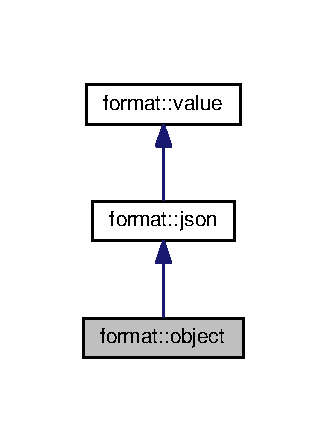
\includegraphics[width=157pt]{classformat_1_1object__inherit__graph}
\end{center}
\end{figure}


Collaboration diagram for format\+:\+:object\+:
\nopagebreak
\begin{figure}[H]
\begin{center}
\leavevmode
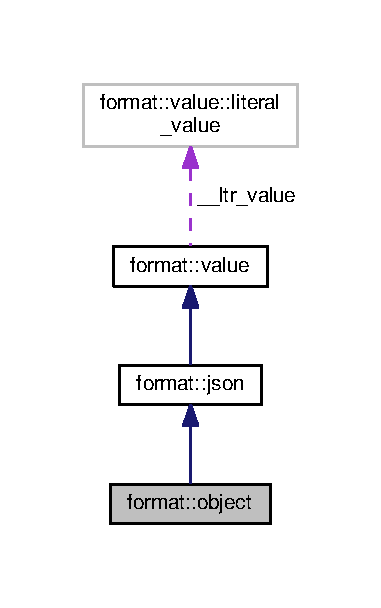
\includegraphics[width=183pt]{classformat_1_1object__coll__graph}
\end{center}
\end{figure}
\subsection*{Classes}
\begin{DoxyCompactItemize}
\item 
class \hyperlink{classformat_1_1object_1_1iterator}{iterator}
\begin{DoxyCompactList}\small\item\em The iterator class. \end{DoxyCompactList}\end{DoxyCompactItemize}
\subsection*{Public Types}
\begin{DoxyCompactItemize}
\item 
typedef std\+::unordered\+\_\+map$<$ std\+::wstring, \hyperlink{classformat_1_1value_aa6b85823936bf7b8ab78d3f8d443c00d}{value} $\ast$ $>$ \hyperlink{classformat_1_1object_a832cdbf5fe57050ca910fd2e98f53e44}{member\+\_\+list}\hypertarget{classformat_1_1object_a832cdbf5fe57050ca910fd2e98f53e44}{}\label{classformat_1_1object_a832cdbf5fe57050ca910fd2e98f53e44}

\begin{DoxyCompactList}\small\item\em member\+\_\+list \end{DoxyCompactList}\end{DoxyCompactItemize}
\subsection*{Public Member Functions}
\begin{DoxyCompactItemize}
\item 
\hyperlink{classformat_1_1object_a70e9c7d76fc5cc4fcc0e0d4612846f11}{object} ()\hypertarget{classformat_1_1object_a70e9c7d76fc5cc4fcc0e0d4612846f11}{}\label{classformat_1_1object_a70e9c7d76fc5cc4fcc0e0d4612846f11}

\begin{DoxyCompactList}\small\item\em object \end{DoxyCompactList}\item 
\hyperlink{classformat_1_1object_a0c0e369bcf4d47f71dda07547bee4d23}{object} (const wchar\+\_\+t $\ast$\hyperlink{classformat_1_1json}{json})
\begin{DoxyCompactList}\small\item\em object \end{DoxyCompactList}\item 
\hyperlink{classformat_1_1object_a662c556b66222187d4f597db0b868404}{object} (std\+::initializer\+\_\+list$<$ std\+::pair$<$ std\+::wstring, \hyperlink{classformat_1_1value_aa6b85823936bf7b8ab78d3f8d443c00d}{value} $\ast$ $>$$>$ il)
\begin{DoxyCompactList}\small\item\em object \end{DoxyCompactList}\item 
\hyperlink{classformat_1_1object_a07b0e1989322aabec4f767cff13be567}{object} (const \hyperlink{classformat_1_1object}{object} \&other)
\begin{DoxyCompactList}\small\item\em object \end{DoxyCompactList}\item 
virtual \hyperlink{classformat_1_1value_aa6b85823936bf7b8ab78d3f8d443c00d}{value} $\ast$ \hyperlink{classformat_1_1object_a3e6550914c83ba0796877e5da8a511bd}{clone} () const override
\begin{DoxyCompactList}\small\item\em clone \end{DoxyCompactList}\item 
virtual \hyperlink{classformat_1_1object_a023704895a984b93cdfe947cf52a2774}{$\sim$object} () override\hypertarget{classformat_1_1object_a023704895a984b93cdfe947cf52a2774}{}\label{classformat_1_1object_a023704895a984b93cdfe947cf52a2774}

\begin{DoxyCompactList}\small\item\em $\sim$object \end{DoxyCompactList}\item 
virtual \hyperlink{classformat_1_1value_aa0334be06389a7b14af485fa0cd3aa21}{value\+\_\+t} \hyperlink{classformat_1_1object_aea7eb835fcbec62a85d078a7fa33cea7}{type} () const noexceptoverride
\begin{DoxyCompactList}\small\item\em type \end{DoxyCompactList}\item 
virtual size\+\_\+t \hyperlink{classformat_1_1object_a29be05a1b87c2d6263f15fc3280e3b6f}{length} () const noexceptoverride
\begin{DoxyCompactList}\small\item\em count \end{DoxyCompactList}\item 
\hyperlink{classformat_1_1value_aa6b85823936bf7b8ab78d3f8d443c00d}{value} \& \hyperlink{classformat_1_1object_a7df33aacd027ccfc4e710397142c7930}{operator=} (const \hyperlink{classformat_1_1object}{object} \&o)
\begin{DoxyCompactList}\small\item\em operator = \end{DoxyCompactList}\item 
virtual size\+\_\+t \hyperlink{classformat_1_1object_a866a470f6092172fcde8307882236a50}{str\+\_\+length} () const noexceptoverride
\begin{DoxyCompactList}\small\item\em str\+\_\+length \end{DoxyCompactList}\item 
\hyperlink{classformat_1_1object_1_1iterator}{iterator} \hyperlink{classformat_1_1object_aae71a75db823350a5a5e19899cd41f74}{begin} ()
\begin{DoxyCompactList}\small\item\em begin \end{DoxyCompactList}\item 
\hyperlink{classformat_1_1object_1_1iterator}{iterator} \hyperlink{classformat_1_1object_ad5c87c9101ca99c51fb19f4a81d1ab09}{end} ()
\begin{DoxyCompactList}\small\item\em end \end{DoxyCompactList}\end{DoxyCompactItemize}
\subsection*{Protected Member Functions}
\begin{DoxyCompactItemize}
\item 
\hyperlink{classformat_1_1object_a458b75773ef8f632e5955fa17ea6eb49}{object} (\hyperlink{classformat_1_1json}{json} $\ast$\hyperlink{classformat_1_1value_a86c03ec8810bfd0d60ec49095120040d}{parent})
\begin{DoxyCompactList}\small\item\em object \end{DoxyCompactList}\item 
virtual \hyperlink{classformat_1_1value_aa6b85823936bf7b8ab78d3f8d443c00d}{value} $\ast$ \hyperlink{classformat_1_1object_ad0de8290132a916e810df0819f6400cb}{\+\_\+clone} (const \hyperlink{classformat_1_1value_aa6b85823936bf7b8ab78d3f8d443c00d}{value} \&other) override
\begin{DoxyCompactList}\small\item\em \+\_\+clone \end{DoxyCompactList}\item 
virtual const wchar\+\_\+t $\ast$ \hyperlink{classformat_1_1object_a6680c7e4b32da5a29d89f2289bb63ee1}{\+\_\+parse} (const wchar\+\_\+t $\ast$\hyperlink{classformat_1_1json}{json}) override
\begin{DoxyCompactList}\small\item\em parse \end{DoxyCompactList}\item 
bool \hyperlink{classformat_1_1object_aac55101129d74838f7181669cdfaa426}{\+\_\+pair} ()
\begin{DoxyCompactList}\small\item\em \+\_\+pair \end{DoxyCompactList}\item 
virtual \hyperlink{classformat_1_1value_aa6b85823936bf7b8ab78d3f8d443c00d}{value} \& \hyperlink{classformat_1_1object_a91e3027c7786c2e24ca3e001f648542d}{\+\_\+at} (const wchar\+\_\+t $\ast$\hyperlink{classformat_1_1value_ad4865e7984fc9f3b5ce7c17fd7ac740c}{key}) override
\begin{DoxyCompactList}\small\item\em \+\_\+at \end{DoxyCompactList}\item 
virtual \hyperlink{classformat_1_1value_aa6b85823936bf7b8ab78d3f8d443c00d}{value} \& \hyperlink{classformat_1_1object_a525bdfa2db22cd6bc21a868a695fe752}{\+\_\+at} (size\+\_\+t) override
\begin{DoxyCompactList}\small\item\em \+\_\+at \end{DoxyCompactList}\item 
virtual \hyperlink{classformat_1_1value_aa6b85823936bf7b8ab78d3f8d443c00d}{value} \& \hyperlink{classformat_1_1object_ad1b5cd15cd7db0d3afba5ec5fa713a1e}{\+\_\+assign} (\hyperlink{classformat_1_1value_aa6b85823936bf7b8ab78d3f8d443c00d}{value} $\ast$ov, \hyperlink{classformat_1_1value_aa6b85823936bf7b8ab78d3f8d443c00d}{value} $\ast$nv) override
\begin{DoxyCompactList}\small\item\em assign \end{DoxyCompactList}\item 
virtual void \hyperlink{classformat_1_1object_ac6db5016da29f906f67d293b27c8bb34}{\+\_\+clear} () override\hypertarget{classformat_1_1object_ac6db5016da29f906f67d293b27c8bb34}{}\label{classformat_1_1object_ac6db5016da29f906f67d293b27c8bb34}

\begin{DoxyCompactList}\small\item\em \+\_\+clear \end{DoxyCompactList}\item 
virtual \hyperlink{classformat_1_1value_aa6b85823936bf7b8ab78d3f8d443c00d}{value} \& \hyperlink{classformat_1_1object_a8da91a2e94cea219e1462d7857f27af7}{\+\_\+erase} (const \hyperlink{classformat_1_1value_aa6b85823936bf7b8ab78d3f8d443c00d}{value} \&v) noexceptoverride
\begin{DoxyCompactList}\small\item\em \+\_\+erase \end{DoxyCompactList}\item 
virtual const wchar\+\_\+t $\ast$ \hyperlink{classformat_1_1object_ade521091c997a1a61e15122364c32e99}{\+\_\+to\+\_\+string} (wchar\+\_\+t $\ast$offset=0) const override
\begin{DoxyCompactList}\small\item\em \+\_\+to\+\_\+str \end{DoxyCompactList}\end{DoxyCompactItemize}
\subsection*{Protected Attributes}
\begin{DoxyCompactItemize}
\item 
\hyperlink{classformat_1_1object_a832cdbf5fe57050ca910fd2e98f53e44}{member\+\_\+list} \hyperlink{classformat_1_1object_ac49dd2aada563d000599673d55effd0b}{\+\_\+member\+\_\+list}\hypertarget{classformat_1_1object_ac49dd2aada563d000599673d55effd0b}{}\label{classformat_1_1object_ac49dd2aada563d000599673d55effd0b}

\begin{DoxyCompactList}\small\item\em \+\_\+member\+\_\+list \end{DoxyCompactList}\end{DoxyCompactItemize}
\subsection*{Friends}
\begin{DoxyCompactItemize}
\item 
\hyperlink{classformat_1_1object}{object} $\ast$ {\bfseries \+\_\+\+\_\+call\+\_\+object} (\hyperlink{classformat_1_1json}{json} $\ast$\hyperlink{classformat_1_1value_a86c03ec8810bfd0d60ec49095120040d}{parent})\hypertarget{classformat_1_1object_aa1c1638285082ba2951a8ff727ce9950}{}\label{classformat_1_1object_aa1c1638285082ba2951a8ff727ce9950}

\end{DoxyCompactItemize}
\subsection*{Additional Inherited Members}


\subsection{Detailed Description}
The object class. 

\subsection{Constructor \& Destructor Documentation}
\index{format\+::object@{format\+::object}!object@{object}}
\index{object@{object}!format\+::object@{format\+::object}}
\subsubsection[{\texorpdfstring{object(const wchar\+\_\+t $\ast$json)}{object(const wchar_t *json)}}]{\setlength{\rightskip}{0pt plus 5cm}format\+::object\+::object (
\begin{DoxyParamCaption}
\item[{const wchar\+\_\+t $\ast$}]{json}
\end{DoxyParamCaption}
)}\hypertarget{classformat_1_1object_a0c0e369bcf4d47f71dda07547bee4d23}{}\label{classformat_1_1object_a0c0e369bcf4d47f71dda07547bee4d23}


object 


\begin{DoxyParams}{Parameters}
{\em json} & \\
\hline
\end{DoxyParams}
\index{format\+::object@{format\+::object}!object@{object}}
\index{object@{object}!format\+::object@{format\+::object}}
\subsubsection[{\texorpdfstring{object(std\+::initializer\+\_\+list$<$ std\+::pair$<$ std\+::wstring, value $\ast$ $>$$>$ il)}{object(std::initializer_list< std::pair< std::wstring, value * >> il)}}]{\setlength{\rightskip}{0pt plus 5cm}format\+::object\+::object (
\begin{DoxyParamCaption}
\item[{std\+::initializer\+\_\+list$<$ std\+::pair$<$ std\+::wstring, {\bf value} $\ast$ $>$$>$}]{il}
\end{DoxyParamCaption}
)}\hypertarget{classformat_1_1object_a662c556b66222187d4f597db0b868404}{}\label{classformat_1_1object_a662c556b66222187d4f597db0b868404}


object 


\begin{DoxyParams}{Parameters}
{\em il} & \\
\hline
\end{DoxyParams}
\index{format\+::object@{format\+::object}!object@{object}}
\index{object@{object}!format\+::object@{format\+::object}}
\subsubsection[{\texorpdfstring{object(const object \&other)}{object(const object &other)}}]{\setlength{\rightskip}{0pt plus 5cm}format\+::object\+::object (
\begin{DoxyParamCaption}
\item[{const {\bf object} \&}]{other}
\end{DoxyParamCaption}
)}\hypertarget{classformat_1_1object_a07b0e1989322aabec4f767cff13be567}{}\label{classformat_1_1object_a07b0e1989322aabec4f767cff13be567}


object 


\begin{DoxyParams}{Parameters}
{\em other} & \\
\hline
\end{DoxyParams}
\index{format\+::object@{format\+::object}!object@{object}}
\index{object@{object}!format\+::object@{format\+::object}}
\subsubsection[{\texorpdfstring{object(json $\ast$parent)}{object(json *parent)}}]{\setlength{\rightskip}{0pt plus 5cm}format\+::object\+::object (
\begin{DoxyParamCaption}
\item[{{\bf json} $\ast$}]{parent}
\end{DoxyParamCaption}
)\hspace{0.3cm}{\ttfamily [protected]}}\hypertarget{classformat_1_1object_a458b75773ef8f632e5955fa17ea6eb49}{}\label{classformat_1_1object_a458b75773ef8f632e5955fa17ea6eb49}


object 


\begin{DoxyParams}{Parameters}
{\em parent} & \\
\hline
\end{DoxyParams}


\subsection{Member Function Documentation}
\index{format\+::object@{format\+::object}!\+\_\+assign@{\+\_\+assign}}
\index{\+\_\+assign@{\+\_\+assign}!format\+::object@{format\+::object}}
\subsubsection[{\texorpdfstring{\+\_\+assign(value $\ast$ov, value $\ast$nv) override}{_assign(value *ov, value *nv) override}}]{\setlength{\rightskip}{0pt plus 5cm}{\bf format\+::value} \& format\+::object\+::\+\_\+assign (
\begin{DoxyParamCaption}
\item[{{\bf value} $\ast$}]{ov, }
\item[{{\bf value} $\ast$}]{nv}
\end{DoxyParamCaption}
)\hspace{0.3cm}{\ttfamily [override]}, {\ttfamily [protected]}, {\ttfamily [virtual]}}\hypertarget{classformat_1_1object_ad1b5cd15cd7db0d3afba5ec5fa713a1e}{}\label{classformat_1_1object_ad1b5cd15cd7db0d3afba5ec5fa713a1e}


assign 


\begin{DoxyParams}{Parameters}
{\em ov} & \\
\hline
{\em nv} & \\
\hline
\end{DoxyParams}


Reimplemented from \hyperlink{classformat_1_1json_a331d385e55541671d431d5e5167e8c90}{format\+::json}.

\index{format\+::object@{format\+::object}!\+\_\+at@{\+\_\+at}}
\index{\+\_\+at@{\+\_\+at}!format\+::object@{format\+::object}}
\subsubsection[{\texorpdfstring{\+\_\+at(const wchar\+\_\+t $\ast$key) override}{_at(const wchar_t *key) override}}]{\setlength{\rightskip}{0pt plus 5cm}{\bf format\+::value} \& format\+::object\+::\+\_\+at (
\begin{DoxyParamCaption}
\item[{const wchar\+\_\+t $\ast$}]{key}
\end{DoxyParamCaption}
)\hspace{0.3cm}{\ttfamily [override]}, {\ttfamily [protected]}, {\ttfamily [virtual]}}\hypertarget{classformat_1_1object_a91e3027c7786c2e24ca3e001f648542d}{}\label{classformat_1_1object_a91e3027c7786c2e24ca3e001f648542d}


\+\_\+at 


\begin{DoxyParams}{Parameters}
{\em key} & \\
\hline
\end{DoxyParams}
\begin{DoxyReturn}{Returns}

\end{DoxyReturn}


Reimplemented from \hyperlink{classformat_1_1json_afcb78dfb597d7d609c66a4d5b6575082}{format\+::json}.

\index{format\+::object@{format\+::object}!\+\_\+at@{\+\_\+at}}
\index{\+\_\+at@{\+\_\+at}!format\+::object@{format\+::object}}
\subsubsection[{\texorpdfstring{\+\_\+at(size\+\_\+t) override}{_at(size_t) override}}]{\setlength{\rightskip}{0pt plus 5cm}virtual {\bf value}\& format\+::object\+::\+\_\+at (
\begin{DoxyParamCaption}
\item[{size\+\_\+t}]{}
\end{DoxyParamCaption}
)\hspace{0.3cm}{\ttfamily [inline]}, {\ttfamily [override]}, {\ttfamily [protected]}, {\ttfamily [virtual]}}\hypertarget{classformat_1_1object_a525bdfa2db22cd6bc21a868a695fe752}{}\label{classformat_1_1object_a525bdfa2db22cd6bc21a868a695fe752}


\+\_\+at 

\begin{DoxyReturn}{Returns}

\end{DoxyReturn}


Reimplemented from \hyperlink{classformat_1_1json_a4a3924d5a112cda2bcee45ddf92a3d52}{format\+::json}.

\index{format\+::object@{format\+::object}!\+\_\+clone@{\+\_\+clone}}
\index{\+\_\+clone@{\+\_\+clone}!format\+::object@{format\+::object}}
\subsubsection[{\texorpdfstring{\+\_\+clone(const value \&other) override}{_clone(const value &other) override}}]{\setlength{\rightskip}{0pt plus 5cm}{\bf format\+::value} $\ast$ format\+::object\+::\+\_\+clone (
\begin{DoxyParamCaption}
\item[{const {\bf value} \&}]{other}
\end{DoxyParamCaption}
)\hspace{0.3cm}{\ttfamily [override]}, {\ttfamily [protected]}, {\ttfamily [virtual]}}\hypertarget{classformat_1_1object_ad0de8290132a916e810df0819f6400cb}{}\label{classformat_1_1object_ad0de8290132a916e810df0819f6400cb}


\+\_\+clone 

\begin{DoxyReturn}{Returns}

\end{DoxyReturn}


Reimplemented from \hyperlink{classformat_1_1json_a4da6b9a624017973c5955d840e61fdb7}{format\+::json}.

\index{format\+::object@{format\+::object}!\+\_\+erase@{\+\_\+erase}}
\index{\+\_\+erase@{\+\_\+erase}!format\+::object@{format\+::object}}
\subsubsection[{\texorpdfstring{\+\_\+erase(const value \&v) noexceptoverride}{_erase(const value &v) noexceptoverride}}]{\setlength{\rightskip}{0pt plus 5cm}{\bf format\+::value} \& format\+::object\+::\+\_\+erase (
\begin{DoxyParamCaption}
\item[{const {\bf value} \&}]{v}
\end{DoxyParamCaption}
)\hspace{0.3cm}{\ttfamily [override]}, {\ttfamily [protected]}, {\ttfamily [virtual]}, {\ttfamily [noexcept]}}\hypertarget{classformat_1_1object_a8da91a2e94cea219e1462d7857f27af7}{}\label{classformat_1_1object_a8da91a2e94cea219e1462d7857f27af7}


\+\_\+erase 


\begin{DoxyParams}{Parameters}
{\em v} & \\
\hline
\end{DoxyParams}
\begin{DoxyReturn}{Returns}

\end{DoxyReturn}


Reimplemented from \hyperlink{classformat_1_1json_adfc8837bee40c5a11809717f8d34b192}{format\+::json}.

\index{format\+::object@{format\+::object}!\+\_\+pair@{\+\_\+pair}}
\index{\+\_\+pair@{\+\_\+pair}!format\+::object@{format\+::object}}
\subsubsection[{\texorpdfstring{\+\_\+pair()}{_pair()}}]{\setlength{\rightskip}{0pt plus 5cm}bool format\+::object\+::\+\_\+pair (
\begin{DoxyParamCaption}
{}
\end{DoxyParamCaption}
)\hspace{0.3cm}{\ttfamily [protected]}}\hypertarget{classformat_1_1object_aac55101129d74838f7181669cdfaa426}{}\label{classformat_1_1object_aac55101129d74838f7181669cdfaa426}


\+\_\+pair 

\begin{DoxyReturn}{Returns}

\end{DoxyReturn}
\index{format\+::object@{format\+::object}!\+\_\+parse@{\+\_\+parse}}
\index{\+\_\+parse@{\+\_\+parse}!format\+::object@{format\+::object}}
\subsubsection[{\texorpdfstring{\+\_\+parse(const wchar\+\_\+t $\ast$json) override}{_parse(const wchar_t *json) override}}]{\setlength{\rightskip}{0pt plus 5cm}const wchar\+\_\+t $\ast$ format\+::object\+::\+\_\+parse (
\begin{DoxyParamCaption}
\item[{const wchar\+\_\+t $\ast$}]{json}
\end{DoxyParamCaption}
)\hspace{0.3cm}{\ttfamily [override]}, {\ttfamily [protected]}, {\ttfamily [virtual]}}\hypertarget{classformat_1_1object_a6680c7e4b32da5a29d89f2289bb63ee1}{}\label{classformat_1_1object_a6680c7e4b32da5a29d89f2289bb63ee1}


parse 


\begin{DoxyParams}{Parameters}
{\em json} & \\
\hline
\end{DoxyParams}
\begin{DoxyReturn}{Returns}

\end{DoxyReturn}


Reimplemented from \hyperlink{classformat_1_1json_ab316c1d4c585610a60d634605a4b871e}{format\+::json}.

\index{format\+::object@{format\+::object}!\+\_\+to\+\_\+string@{\+\_\+to\+\_\+string}}
\index{\+\_\+to\+\_\+string@{\+\_\+to\+\_\+string}!format\+::object@{format\+::object}}
\subsubsection[{\texorpdfstring{\+\_\+to\+\_\+string(wchar\+\_\+t $\ast$offset=0) const override}{_to_string(wchar_t *offset=0) const override}}]{\setlength{\rightskip}{0pt plus 5cm}const wchar\+\_\+t $\ast$ format\+::object\+::\+\_\+to\+\_\+string (
\begin{DoxyParamCaption}
\item[{wchar\+\_\+t $\ast$}]{offset = {\ttfamily 0}}
\end{DoxyParamCaption}
) const\hspace{0.3cm}{\ttfamily [override]}, {\ttfamily [protected]}, {\ttfamily [virtual]}}\hypertarget{classformat_1_1object_ade521091c997a1a61e15122364c32e99}{}\label{classformat_1_1object_ade521091c997a1a61e15122364c32e99}


\+\_\+to\+\_\+str 


\begin{DoxyParams}{Parameters}
{\em offset} & \\
\hline
\end{DoxyParams}
\begin{DoxyReturn}{Returns}

\end{DoxyReturn}


Reimplemented from \hyperlink{classformat_1_1json_afbb5d88bc2005d89b287e05d89fb2e06}{format\+::json}.

\index{format\+::object@{format\+::object}!begin@{begin}}
\index{begin@{begin}!format\+::object@{format\+::object}}
\subsubsection[{\texorpdfstring{begin()}{begin()}}]{\setlength{\rightskip}{0pt plus 5cm}{\bf iterator} format\+::object\+::begin (
\begin{DoxyParamCaption}
{}
\end{DoxyParamCaption}
)\hspace{0.3cm}{\ttfamily [inline]}}\hypertarget{classformat_1_1object_aae71a75db823350a5a5e19899cd41f74}{}\label{classformat_1_1object_aae71a75db823350a5a5e19899cd41f74}


begin 

\begin{DoxyReturn}{Returns}

\end{DoxyReturn}
\index{format\+::object@{format\+::object}!clone@{clone}}
\index{clone@{clone}!format\+::object@{format\+::object}}
\subsubsection[{\texorpdfstring{clone() const override}{clone() const override}}]{\setlength{\rightskip}{0pt plus 5cm}virtual {\bf value}$\ast$ format\+::object\+::clone (
\begin{DoxyParamCaption}
{}
\end{DoxyParamCaption}
) const\hspace{0.3cm}{\ttfamily [inline]}, {\ttfamily [override]}, {\ttfamily [virtual]}}\hypertarget{classformat_1_1object_a3e6550914c83ba0796877e5da8a511bd}{}\label{classformat_1_1object_a3e6550914c83ba0796877e5da8a511bd}


clone 

\begin{DoxyReturn}{Returns}

\end{DoxyReturn}


Reimplemented from \hyperlink{classformat_1_1json_a49534b733831b2dae879d7407f7cfba5}{format\+::json}.

\index{format\+::object@{format\+::object}!end@{end}}
\index{end@{end}!format\+::object@{format\+::object}}
\subsubsection[{\texorpdfstring{end()}{end()}}]{\setlength{\rightskip}{0pt plus 5cm}{\bf iterator} format\+::object\+::end (
\begin{DoxyParamCaption}
{}
\end{DoxyParamCaption}
)\hspace{0.3cm}{\ttfamily [inline]}}\hypertarget{classformat_1_1object_ad5c87c9101ca99c51fb19f4a81d1ab09}{}\label{classformat_1_1object_ad5c87c9101ca99c51fb19f4a81d1ab09}


end 

\begin{DoxyReturn}{Returns}

\end{DoxyReturn}
\index{format\+::object@{format\+::object}!length@{length}}
\index{length@{length}!format\+::object@{format\+::object}}
\subsubsection[{\texorpdfstring{length() const noexceptoverride}{length() const noexceptoverride}}]{\setlength{\rightskip}{0pt plus 5cm}virtual size\+\_\+t format\+::object\+::length (
\begin{DoxyParamCaption}
{}
\end{DoxyParamCaption}
) const\hspace{0.3cm}{\ttfamily [inline]}, {\ttfamily [override]}, {\ttfamily [virtual]}, {\ttfamily [noexcept]}}\hypertarget{classformat_1_1object_a29be05a1b87c2d6263f15fc3280e3b6f}{}\label{classformat_1_1object_a29be05a1b87c2d6263f15fc3280e3b6f}


count 

\begin{DoxyReturn}{Returns}

\end{DoxyReturn}


Reimplemented from \hyperlink{classformat_1_1json_a792f3755d148f250ae60e4bbb35fbc6b}{format\+::json}.

\index{format\+::object@{format\+::object}!operator=@{operator=}}
\index{operator=@{operator=}!format\+::object@{format\+::object}}
\subsubsection[{\texorpdfstring{operator=(const object \&o)}{operator=(const object &o)}}]{\setlength{\rightskip}{0pt plus 5cm}{\bf value}\& format\+::object\+::operator= (
\begin{DoxyParamCaption}
\item[{const {\bf object} \&}]{o}
\end{DoxyParamCaption}
)\hspace{0.3cm}{\ttfamily [inline]}}\hypertarget{classformat_1_1object_a7df33aacd027ccfc4e710397142c7930}{}\label{classformat_1_1object_a7df33aacd027ccfc4e710397142c7930}


operator = 


\begin{DoxyParams}{Parameters}
{\em o} & \\
\hline
\end{DoxyParams}
\begin{DoxyReturn}{Returns}

\end{DoxyReturn}
\index{format\+::object@{format\+::object}!str\+\_\+length@{str\+\_\+length}}
\index{str\+\_\+length@{str\+\_\+length}!format\+::object@{format\+::object}}
\subsubsection[{\texorpdfstring{str\+\_\+length() const noexceptoverride}{str_length() const noexceptoverride}}]{\setlength{\rightskip}{0pt plus 5cm}size\+\_\+t format\+::object\+::str\+\_\+length (
\begin{DoxyParamCaption}
{}
\end{DoxyParamCaption}
) const\hspace{0.3cm}{\ttfamily [override]}, {\ttfamily [virtual]}, {\ttfamily [noexcept]}}\hypertarget{classformat_1_1object_a866a470f6092172fcde8307882236a50}{}\label{classformat_1_1object_a866a470f6092172fcde8307882236a50}


str\+\_\+length 

\begin{DoxyReturn}{Returns}

\end{DoxyReturn}


Reimplemented from \hyperlink{classformat_1_1json_a1110e453dd28d55ed9b6b196d04d1c7e}{format\+::json}.

\index{format\+::object@{format\+::object}!type@{type}}
\index{type@{type}!format\+::object@{format\+::object}}
\subsubsection[{\texorpdfstring{type() const noexceptoverride}{type() const noexceptoverride}}]{\setlength{\rightskip}{0pt plus 5cm}virtual {\bf value\+\_\+t} format\+::object\+::type (
\begin{DoxyParamCaption}
{}
\end{DoxyParamCaption}
) const\hspace{0.3cm}{\ttfamily [inline]}, {\ttfamily [override]}, {\ttfamily [virtual]}, {\ttfamily [noexcept]}}\hypertarget{classformat_1_1object_aea7eb835fcbec62a85d078a7fa33cea7}{}\label{classformat_1_1object_aea7eb835fcbec62a85d078a7fa33cea7}


type 

\begin{DoxyReturn}{Returns}

\end{DoxyReturn}


Reimplemented from \hyperlink{classformat_1_1json_a970027799aac71bf99e3f1d7264364dc}{format\+::json}.



The documentation for this class was generated from the following files\+:\begin{DoxyCompactItemize}
\item 
json\+\_\+object.\+h\item 
json\+\_\+object.\+cpp\end{DoxyCompactItemize}

\hypertarget{classformat_1_1string}{}\section{format\+:\+:string Class Reference}
\label{classformat_1_1string}\index{format\+::string@{format\+::string}}


The string class.  




{\ttfamily \#include $<$json\+\_\+string.\+h$>$}



Inheritance diagram for format\+:\+:string\+:
\nopagebreak
\begin{figure}[H]
\begin{center}
\leavevmode
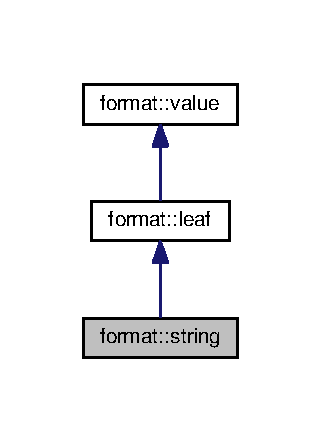
\includegraphics[width=154pt]{classformat_1_1string__inherit__graph}
\end{center}
\end{figure}


Collaboration diagram for format\+:\+:string\+:
\nopagebreak
\begin{figure}[H]
\begin{center}
\leavevmode
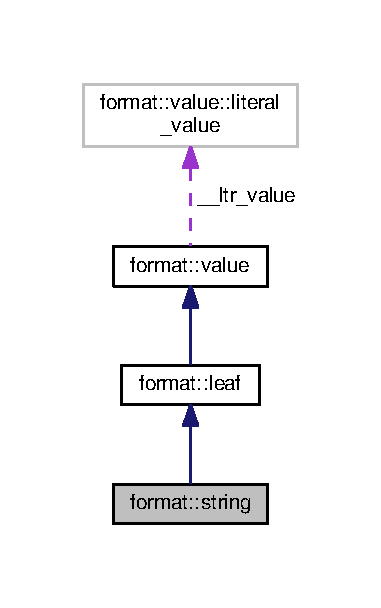
\includegraphics[width=183pt]{classformat_1_1string__coll__graph}
\end{center}
\end{figure}
\subsection*{Public Member Functions}
\begin{DoxyCompactItemize}
\item 
\hyperlink{classformat_1_1string_a39d80d4824791541f07d92e907c90c24}{string} ()\hypertarget{classformat_1_1string_a39d80d4824791541f07d92e907c90c24}{}\label{classformat_1_1string_a39d80d4824791541f07d92e907c90c24}

\begin{DoxyCompactList}\small\item\em String. \end{DoxyCompactList}\item 
\hyperlink{classformat_1_1string_a38c53c8153cd7dadc295329b32ba0ffd}{string} (const wchar\+\_\+t $\ast$\hyperlink{classformat_1_1json}{json})
\begin{DoxyCompactList}\small\item\em String. \end{DoxyCompactList}\item 
\hyperlink{classformat_1_1string_a46c207d7796b70808e571e14f1379df8}{string} (const \hyperlink{classformat_1_1string}{string} \&other)
\begin{DoxyCompactList}\small\item\em String. \end{DoxyCompactList}\item 
virtual \hyperlink{classformat_1_1string_af7dcae7eff45b579ffa8dd47d82326ca}{$\sim$string} () override=default\hypertarget{classformat_1_1string_af7dcae7eff45b579ffa8dd47d82326ca}{}\label{classformat_1_1string_af7dcae7eff45b579ffa8dd47d82326ca}

\begin{DoxyCompactList}\small\item\em $\sim$string \end{DoxyCompactList}\item 
virtual \hyperlink{classformat_1_1value_aa6b85823936bf7b8ab78d3f8d443c00d}{value} $\ast$ \hyperlink{classformat_1_1string_a41b0ffc3e1c686bc07fbe911942a0a4f}{clone} () const override
\begin{DoxyCompactList}\small\item\em clone \end{DoxyCompactList}\item 
virtual \hyperlink{classformat_1_1value_aa0334be06389a7b14af485fa0cd3aa21}{value\+\_\+t} \hyperlink{classformat_1_1string_a247e17aaf8cb8e0afdc29e943d492232}{type} () const noexceptoverride
\begin{DoxyCompactList}\small\item\em type \end{DoxyCompactList}\item 
\hyperlink{classformat_1_1value_aa6b85823936bf7b8ab78d3f8d443c00d}{value} \& \hyperlink{classformat_1_1string_a6b45888b8f15e35546b7f0f0007a795c}{operator=} (const \hyperlink{classformat_1_1string}{string} \&s)
\begin{DoxyCompactList}\small\item\em operator = \end{DoxyCompactList}\item 
const wchar\+\_\+t $\ast$ \hyperlink{classformat_1_1string_af8468eab8f5499b2f1bfde6a680fab47}{get} () const 
\begin{DoxyCompactList}\small\item\em value \end{DoxyCompactList}\item 
virtual size\+\_\+t \hyperlink{classformat_1_1string_a6447b6867f08a78e0bd82cc7c63d2f6e}{str\+\_\+length} () const noexceptoverride
\begin{DoxyCompactList}\small\item\em str\+Length \end{DoxyCompactList}\end{DoxyCompactItemize}
\subsection*{Protected Member Functions}
\begin{DoxyCompactItemize}
\item 
\hyperlink{classformat_1_1string_a264d5b290279be616e7f48c54a295635}{string} (\hyperlink{classformat_1_1json}{json} $\ast$\hyperlink{classformat_1_1value_a86c03ec8810bfd0d60ec49095120040d}{parent}, size\+\_\+t charc)
\begin{DoxyCompactList}\small\item\em string \end{DoxyCompactList}\item 
virtual const wchar\+\_\+t $\ast$ \hyperlink{classformat_1_1string_a1a3b05c60c4cc387d4a37956f20a56f3}{\+\_\+parse} (const wchar\+\_\+t $\ast$\hyperlink{classformat_1_1json}{json}) override
\begin{DoxyCompactList}\small\item\em parse \end{DoxyCompactList}\item 
virtual void \hyperlink{classformat_1_1string_a3217635d20a78516525fd6adb59576fb}{\+\_\+clear} () override
\begin{DoxyCompactList}\small\item\em \+\_\+copy \end{DoxyCompactList}\item 
virtual \hyperlink{classformat_1_1value_aa6b85823936bf7b8ab78d3f8d443c00d}{value} $\ast$ \hyperlink{classformat_1_1string_a876061b10e5edf4d8ba9801bf819f8c9}{\+\_\+clone} (const \hyperlink{classformat_1_1value_aa6b85823936bf7b8ab78d3f8d443c00d}{value} \&nv) override
\begin{DoxyCompactList}\small\item\em \+\_\+clone \end{DoxyCompactList}\item 
\hyperlink{classformat_1_1value_aa6b85823936bf7b8ab78d3f8d443c00d}{value} \& \hyperlink{classformat_1_1string_adafebf74fd93cb4929a9cee1f13765c3}{\+\_\+assign} (const \hyperlink{classformat_1_1string}{string} \&nv)
\begin{DoxyCompactList}\small\item\em assign \end{DoxyCompactList}\item 
virtual const wchar\+\_\+t $\ast$ \hyperlink{classformat_1_1string_a4522fce4f8002088bccdcb7b2aba53b6}{\+\_\+to\+\_\+string} (wchar\+\_\+t $\ast$=0) const override
\begin{DoxyCompactList}\small\item\em str\+Value \end{DoxyCompactList}\end{DoxyCompactItemize}
\subsection*{Protected Attributes}
\begin{DoxyCompactItemize}
\item 
const wchar\+\_\+t $\ast$ \hyperlink{classformat_1_1string_a33f5dbb40ce3ad6361384c0b543fb216}{\+\_\+startp}\hypertarget{classformat_1_1string_a33f5dbb40ce3ad6361384c0b543fb216}{}\label{classformat_1_1string_a33f5dbb40ce3ad6361384c0b543fb216}

\begin{DoxyCompactList}\small\item\em \+\_\+startp \end{DoxyCompactList}\item 
size\+\_\+t \hyperlink{classformat_1_1string_a7622ab780e0a919908d314b173012f41}{\+\_\+charc}\hypertarget{classformat_1_1string_a7622ab780e0a919908d314b173012f41}{}\label{classformat_1_1string_a7622ab780e0a919908d314b173012f41}

\begin{DoxyCompactList}\small\item\em \+\_\+charc \end{DoxyCompactList}\item 
std\+::wstring \hyperlink{classformat_1_1string_ad953f26ee9500cbcd166df27ae7fb7a4}{\+\_\+string\+\_\+value} \mbox{[}2\mbox{]}\hypertarget{classformat_1_1string_ad953f26ee9500cbcd166df27ae7fb7a4}{}\label{classformat_1_1string_ad953f26ee9500cbcd166df27ae7fb7a4}

\begin{DoxyCompactList}\small\item\em \+\_\+value \end{DoxyCompactList}\end{DoxyCompactItemize}
\subsection*{Friends}
\begin{DoxyCompactItemize}
\item 
\hyperlink{classformat_1_1string}{string} $\ast$ \hyperlink{classformat_1_1string_ab6663097ece046a209a089cf9745efc4}{\+\_\+\+\_\+call\+\_\+string} (\hyperlink{classformat_1_1json}{json} $\ast$\hyperlink{classformat_1_1value_a86c03ec8810bfd0d60ec49095120040d}{parent}, size\+\_\+t charc)
\begin{DoxyCompactList}\small\item\em call\+\_\+string \end{DoxyCompactList}\end{DoxyCompactItemize}
\subsection*{Additional Inherited Members}


\subsection{Detailed Description}
The string class. 

\subsection{Constructor \& Destructor Documentation}
\index{format\+::string@{format\+::string}!string@{string}}
\index{string@{string}!format\+::string@{format\+::string}}
\subsubsection[{\texorpdfstring{string(const wchar\+\_\+t $\ast$json)}{string(const wchar_t *json)}}]{\setlength{\rightskip}{0pt plus 5cm}format\+::string\+::string (
\begin{DoxyParamCaption}
\item[{const wchar\+\_\+t $\ast$}]{json}
\end{DoxyParamCaption}
)}\hypertarget{classformat_1_1string_a38c53c8153cd7dadc295329b32ba0ffd}{}\label{classformat_1_1string_a38c53c8153cd7dadc295329b32ba0ffd}


String. 


\begin{DoxyParams}{Parameters}
{\em json} & \\
\hline
\end{DoxyParams}
\index{format\+::string@{format\+::string}!string@{string}}
\index{string@{string}!format\+::string@{format\+::string}}
\subsubsection[{\texorpdfstring{string(const string \&other)}{string(const string &other)}}]{\setlength{\rightskip}{0pt plus 5cm}format\+::string\+::string (
\begin{DoxyParamCaption}
\item[{const {\bf string} \&}]{other}
\end{DoxyParamCaption}
)}\hypertarget{classformat_1_1string_a46c207d7796b70808e571e14f1379df8}{}\label{classformat_1_1string_a46c207d7796b70808e571e14f1379df8}


String. 


\begin{DoxyParams}{Parameters}
{\em other} & \\
\hline
\end{DoxyParams}
\index{format\+::string@{format\+::string}!string@{string}}
\index{string@{string}!format\+::string@{format\+::string}}
\subsubsection[{\texorpdfstring{string(json $\ast$parent, size\+\_\+t charc)}{string(json *parent, size_t charc)}}]{\setlength{\rightskip}{0pt plus 5cm}format\+::string\+::string (
\begin{DoxyParamCaption}
\item[{{\bf json} $\ast$}]{parent, }
\item[{size\+\_\+t}]{charc}
\end{DoxyParamCaption}
)\hspace{0.3cm}{\ttfamily [protected]}}\hypertarget{classformat_1_1string_a264d5b290279be616e7f48c54a295635}{}\label{classformat_1_1string_a264d5b290279be616e7f48c54a295635}


string 


\begin{DoxyParams}{Parameters}
{\em parent} & \\
\hline
{\em charc} & \\
\hline
\end{DoxyParams}


\subsection{Member Function Documentation}
\index{format\+::string@{format\+::string}!\+\_\+assign@{\+\_\+assign}}
\index{\+\_\+assign@{\+\_\+assign}!format\+::string@{format\+::string}}
\subsubsection[{\texorpdfstring{\+\_\+assign(const string \&nv)}{_assign(const string &nv)}}]{\setlength{\rightskip}{0pt plus 5cm}{\bf format\+::value} \& format\+::string\+::\+\_\+assign (
\begin{DoxyParamCaption}
\item[{const {\bf string} \&}]{nv}
\end{DoxyParamCaption}
)\hspace{0.3cm}{\ttfamily [protected]}}\hypertarget{classformat_1_1string_adafebf74fd93cb4929a9cee1f13765c3}{}\label{classformat_1_1string_adafebf74fd93cb4929a9cee1f13765c3}


assign 


\begin{DoxyParams}{Parameters}
{\em nv} & \\
\hline
\end{DoxyParams}
\begin{DoxyReturn}{Returns}

\end{DoxyReturn}
\index{format\+::string@{format\+::string}!\+\_\+clear@{\+\_\+clear}}
\index{\+\_\+clear@{\+\_\+clear}!format\+::string@{format\+::string}}
\subsubsection[{\texorpdfstring{\+\_\+clear() override}{_clear() override}}]{\setlength{\rightskip}{0pt plus 5cm}virtual void format\+::string\+::\+\_\+clear (
\begin{DoxyParamCaption}
{}
\end{DoxyParamCaption}
)\hspace{0.3cm}{\ttfamily [inline]}, {\ttfamily [override]}, {\ttfamily [protected]}, {\ttfamily [virtual]}}\hypertarget{classformat_1_1string_a3217635d20a78516525fd6adb59576fb}{}\label{classformat_1_1string_a3217635d20a78516525fd6adb59576fb}


\+\_\+copy 


\begin{DoxyParams}{Parameters}
{\em nv} & void \+\_\+copy (const String \&nv); \+\_\+clear \\
\hline
\end{DoxyParams}


Implements \hyperlink{classformat_1_1leaf_a98449fdebba18260ac00319e3ad7298f}{format\+::leaf}.

\index{format\+::string@{format\+::string}!\+\_\+clone@{\+\_\+clone}}
\index{\+\_\+clone@{\+\_\+clone}!format\+::string@{format\+::string}}
\subsubsection[{\texorpdfstring{\+\_\+clone(const value \&nv) override}{_clone(const value &nv) override}}]{\setlength{\rightskip}{0pt plus 5cm}{\bf format\+::value} $\ast$ format\+::string\+::\+\_\+clone (
\begin{DoxyParamCaption}
\item[{const {\bf value} \&}]{nv}
\end{DoxyParamCaption}
)\hspace{0.3cm}{\ttfamily [override]}, {\ttfamily [protected]}, {\ttfamily [virtual]}}\hypertarget{classformat_1_1string_a876061b10e5edf4d8ba9801bf819f8c9}{}\label{classformat_1_1string_a876061b10e5edf4d8ba9801bf819f8c9}


\+\_\+clone 

\begin{DoxyReturn}{Returns}

\end{DoxyReturn}


Implements \hyperlink{classformat_1_1leaf_a45f6e4e09027122e445ba3b8352aec14}{format\+::leaf}.

\index{format\+::string@{format\+::string}!\+\_\+parse@{\+\_\+parse}}
\index{\+\_\+parse@{\+\_\+parse}!format\+::string@{format\+::string}}
\subsubsection[{\texorpdfstring{\+\_\+parse(const wchar\+\_\+t $\ast$json) override}{_parse(const wchar_t *json) override}}]{\setlength{\rightskip}{0pt plus 5cm}const wchar\+\_\+t $\ast$ format\+::string\+::\+\_\+parse (
\begin{DoxyParamCaption}
\item[{const wchar\+\_\+t $\ast$}]{json}
\end{DoxyParamCaption}
)\hspace{0.3cm}{\ttfamily [override]}, {\ttfamily [protected]}, {\ttfamily [virtual]}}\hypertarget{classformat_1_1string_a1a3b05c60c4cc387d4a37956f20a56f3}{}\label{classformat_1_1string_a1a3b05c60c4cc387d4a37956f20a56f3}


parse 


\begin{DoxyParams}{Parameters}
{\em json} & \\
\hline
\end{DoxyParams}
\begin{DoxyReturn}{Returns}

\end{DoxyReturn}


Implements \hyperlink{classformat_1_1value_a7859b1aa48f667a83e091f0eba22d4a1}{format\+::value}.

\index{format\+::string@{format\+::string}!\+\_\+to\+\_\+string@{\+\_\+to\+\_\+string}}
\index{\+\_\+to\+\_\+string@{\+\_\+to\+\_\+string}!format\+::string@{format\+::string}}
\subsubsection[{\texorpdfstring{\+\_\+to\+\_\+string(wchar\+\_\+t $\ast$=0) const override}{_to_string(wchar_t *=0) const override}}]{\setlength{\rightskip}{0pt plus 5cm}const wchar\+\_\+t $\ast$ format\+::string\+::\+\_\+to\+\_\+string (
\begin{DoxyParamCaption}
\item[{wchar\+\_\+t $\ast$}]{ = {\ttfamily 0}}
\end{DoxyParamCaption}
) const\hspace{0.3cm}{\ttfamily [override]}, {\ttfamily [protected]}, {\ttfamily [virtual]}}\hypertarget{classformat_1_1string_a4522fce4f8002088bccdcb7b2aba53b6}{}\label{classformat_1_1string_a4522fce4f8002088bccdcb7b2aba53b6}


str\+Value 

\begin{DoxyReturn}{Returns}

\end{DoxyReturn}


Implements \hyperlink{classformat_1_1value_a94ed31f07b19866495297472accd33a8}{format\+::value}.

\index{format\+::string@{format\+::string}!clone@{clone}}
\index{clone@{clone}!format\+::string@{format\+::string}}
\subsubsection[{\texorpdfstring{clone() const override}{clone() const override}}]{\setlength{\rightskip}{0pt plus 5cm}virtual {\bf value}$\ast$ format\+::string\+::clone (
\begin{DoxyParamCaption}
{}
\end{DoxyParamCaption}
) const\hspace{0.3cm}{\ttfamily [inline]}, {\ttfamily [override]}, {\ttfamily [virtual]}}\hypertarget{classformat_1_1string_a41b0ffc3e1c686bc07fbe911942a0a4f}{}\label{classformat_1_1string_a41b0ffc3e1c686bc07fbe911942a0a4f}


clone 


\begin{DoxyParams}{Parameters}
{\em other} & \\
\hline
\end{DoxyParams}
\begin{DoxyReturn}{Returns}

\end{DoxyReturn}


Implements \hyperlink{classformat_1_1leaf_a861972c1866ab17d00e4b950d33d4ced}{format\+::leaf}.

\index{format\+::string@{format\+::string}!get@{get}}
\index{get@{get}!format\+::string@{format\+::string}}
\subsubsection[{\texorpdfstring{get() const }{get() const }}]{\setlength{\rightskip}{0pt plus 5cm}const wchar\+\_\+t $\ast$ format\+::string\+::get (
\begin{DoxyParamCaption}
{}
\end{DoxyParamCaption}
) const}\hypertarget{classformat_1_1string_af8468eab8f5499b2f1bfde6a680fab47}{}\label{classformat_1_1string_af8468eab8f5499b2f1bfde6a680fab47}


value 

\begin{DoxyReturn}{Returns}

\end{DoxyReturn}
\index{format\+::string@{format\+::string}!operator=@{operator=}}
\index{operator=@{operator=}!format\+::string@{format\+::string}}
\subsubsection[{\texorpdfstring{operator=(const string \&s)}{operator=(const string &s)}}]{\setlength{\rightskip}{0pt plus 5cm}{\bf value}\& format\+::string\+::operator= (
\begin{DoxyParamCaption}
\item[{const {\bf string} \&}]{s}
\end{DoxyParamCaption}
)\hspace{0.3cm}{\ttfamily [inline]}}\hypertarget{classformat_1_1string_a6b45888b8f15e35546b7f0f0007a795c}{}\label{classformat_1_1string_a6b45888b8f15e35546b7f0f0007a795c}


operator = 


\begin{DoxyParams}{Parameters}
{\em s} & \\
\hline
\end{DoxyParams}
\begin{DoxyReturn}{Returns}

\end{DoxyReturn}
\index{format\+::string@{format\+::string}!str\+\_\+length@{str\+\_\+length}}
\index{str\+\_\+length@{str\+\_\+length}!format\+::string@{format\+::string}}
\subsubsection[{\texorpdfstring{str\+\_\+length() const noexceptoverride}{str_length() const noexceptoverride}}]{\setlength{\rightskip}{0pt plus 5cm}virtual size\+\_\+t format\+::string\+::str\+\_\+length (
\begin{DoxyParamCaption}
{}
\end{DoxyParamCaption}
) const\hspace{0.3cm}{\ttfamily [inline]}, {\ttfamily [override]}, {\ttfamily [virtual]}, {\ttfamily [noexcept]}}\hypertarget{classformat_1_1string_a6447b6867f08a78e0bd82cc7c63d2f6e}{}\label{classformat_1_1string_a6447b6867f08a78e0bd82cc7c63d2f6e}


str\+Length 

\begin{DoxyReturn}{Returns}

\end{DoxyReturn}


Implements \hyperlink{classformat_1_1value_a399280e27e629db0582b5781b90ca58b}{format\+::value}.

\index{format\+::string@{format\+::string}!type@{type}}
\index{type@{type}!format\+::string@{format\+::string}}
\subsubsection[{\texorpdfstring{type() const noexceptoverride}{type() const noexceptoverride}}]{\setlength{\rightskip}{0pt plus 5cm}virtual {\bf value\+\_\+t} format\+::string\+::type (
\begin{DoxyParamCaption}
{}
\end{DoxyParamCaption}
) const\hspace{0.3cm}{\ttfamily [inline]}, {\ttfamily [override]}, {\ttfamily [virtual]}, {\ttfamily [noexcept]}}\hypertarget{classformat_1_1string_a247e17aaf8cb8e0afdc29e943d492232}{}\label{classformat_1_1string_a247e17aaf8cb8e0afdc29e943d492232}


type 

\begin{DoxyReturn}{Returns}

\end{DoxyReturn}


Implements \hyperlink{classformat_1_1leaf_ac29de88719f2da4d262255ef8a234ced}{format\+::leaf}.



\subsection{Friends And Related Function Documentation}
\index{format\+::string@{format\+::string}!\+\_\+\+\_\+call\+\_\+string@{\+\_\+\+\_\+call\+\_\+string}}
\index{\+\_\+\+\_\+call\+\_\+string@{\+\_\+\+\_\+call\+\_\+string}!format\+::string@{format\+::string}}
\subsubsection[{\texorpdfstring{\+\_\+\+\_\+call\+\_\+string}{__call_string}}]{\setlength{\rightskip}{0pt plus 5cm}{\bf string}$\ast$ \+\_\+\+\_\+call\+\_\+string (
\begin{DoxyParamCaption}
\item[{{\bf json} $\ast$}]{parent, }
\item[{size\+\_\+t}]{charc}
\end{DoxyParamCaption}
)\hspace{0.3cm}{\ttfamily [friend]}}\hypertarget{classformat_1_1string_ab6663097ece046a209a089cf9745efc4}{}\label{classformat_1_1string_ab6663097ece046a209a089cf9745efc4}


call\+\_\+string 


\begin{DoxyParams}{Parameters}
{\em parent} & \\
\hline
{\em charc} & \\
\hline
\end{DoxyParams}
\begin{DoxyReturn}{Returns}

\end{DoxyReturn}


The documentation for this class was generated from the following files\+:\begin{DoxyCompactItemize}
\item 
json\+\_\+string.\+h\item 
json\+\_\+string.\+cpp\end{DoxyCompactItemize}

\hypertarget{classformat_1_1undefined}{}\section{format\+:\+:undefined Class Reference}
\label{classformat_1_1undefined}\index{format\+::undefined@{format\+::undefined}}


The undefined class.  




{\ttfamily \#include $<$json\+\_\+undefined.\+h$>$}



Inheritance diagram for format\+:\+:undefined\+:
\nopagebreak
\begin{figure}[H]
\begin{center}
\leavevmode
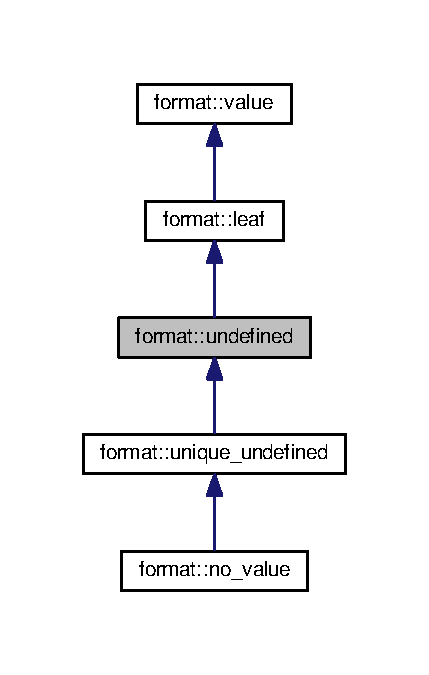
\includegraphics[width=206pt]{classformat_1_1undefined__inherit__graph}
\end{center}
\end{figure}


Collaboration diagram for format\+:\+:undefined\+:
\nopagebreak
\begin{figure}[H]
\begin{center}
\leavevmode
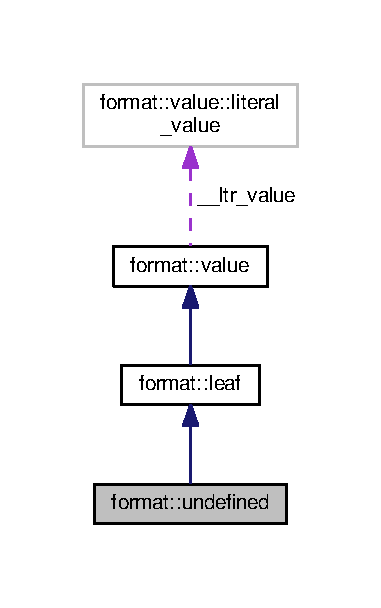
\includegraphics[width=183pt]{classformat_1_1undefined__coll__graph}
\end{center}
\end{figure}
\subsection*{Public Member Functions}
\begin{DoxyCompactItemize}
\item 
\hyperlink{classformat_1_1undefined_aeeee6253ddd4623b960d268222a61960}{undefined} (\hyperlink{classformat_1_1json}{json} $\ast$\hyperlink{classformat_1_1value_a86c03ec8810bfd0d60ec49095120040d}{parent})
\begin{DoxyCompactList}\small\item\em Undefined. \end{DoxyCompactList}\item 
\hyperlink{classformat_1_1undefined_a3a95a41b5fa665df9cd1d577ef1b5d2d}{undefined} (const \hyperlink{classformat_1_1undefined}{undefined} \&other)=default
\begin{DoxyCompactList}\small\item\em Undefined. \end{DoxyCompactList}\item 
virtual \hyperlink{classformat_1_1undefined_a9f05b932696e3e6b690b1ac29de3ed95}{$\sim$undefined} () override=default\hypertarget{classformat_1_1undefined_a9f05b932696e3e6b690b1ac29de3ed95}{}\label{classformat_1_1undefined_a9f05b932696e3e6b690b1ac29de3ed95}

\begin{DoxyCompactList}\small\item\em $\sim$undefined \end{DoxyCompactList}\item 
void \hyperlink{classformat_1_1undefined_a0338d8a0155940468e5e075e2ac70312}{operator delete} (void $\ast$)\hypertarget{classformat_1_1undefined_a0338d8a0155940468e5e075e2ac70312}{}\label{classformat_1_1undefined_a0338d8a0155940468e5e075e2ac70312}

\begin{DoxyCompactList}\small\item\em operator delete \end{DoxyCompactList}\item 
void \hyperlink{classformat_1_1undefined_ad3f119cd1bf17f5735d03dd92590b6d5}{operator delete\mbox{[}$\,$\mbox{]}} (void $\ast$)\hypertarget{classformat_1_1undefined_ad3f119cd1bf17f5735d03dd92590b6d5}{}\label{classformat_1_1undefined_ad3f119cd1bf17f5735d03dd92590b6d5}

\begin{DoxyCompactList}\small\item\em operator delete\mbox{[}\mbox{]} \end{DoxyCompactList}\item 
virtual \hyperlink{classformat_1_1value_aa6b85823936bf7b8ab78d3f8d443c00d}{value} $\ast$ \hyperlink{classformat_1_1undefined_af418bdce70e2d41131ac640fcf6dc121}{clone} () const 
\begin{DoxyCompactList}\small\item\em clone \end{DoxyCompactList}\item 
std\+::nullptr\+\_\+t \hyperlink{classformat_1_1undefined_a18a92924d0ce07768762f6ea64188a19}{get} () const noexcept
\begin{DoxyCompactList}\small\item\em get \end{DoxyCompactList}\item 
virtual const wchar\+\_\+t $\ast$ \hyperlink{classformat_1_1undefined_a407a10b3bfa670b2a8b1e3b8ef6cf698}{\+\_\+parse} (const wchar\+\_\+t $\ast$\hyperlink{classformat_1_1json}{json}) override
\begin{DoxyCompactList}\small\item\em parse \end{DoxyCompactList}\item 
virtual \hyperlink{classformat_1_1value_aa0334be06389a7b14af485fa0cd3aa21}{value\+\_\+t} \hyperlink{classformat_1_1undefined_a72e4ff819514b2a4126be1969d5bbabe}{type} () const noexceptoverride
\begin{DoxyCompactList}\small\item\em type \end{DoxyCompactList}\item 
virtual size\+\_\+t \hyperlink{classformat_1_1undefined_a94e5461ec5938de5aae6de2e0e9ea604}{str\+\_\+length} () const noexceptoverride
\begin{DoxyCompactList}\small\item\em str\+Length \end{DoxyCompactList}\end{DoxyCompactItemize}
\subsection*{Static Public Member Functions}
\begin{DoxyCompactItemize}
\item 
static void $\ast$ \hyperlink{classformat_1_1undefined_a574db8ca686c0072c8af1c10aad45df6}{operator new} (std\+::size\+\_\+t size)
\begin{DoxyCompactList}\small\item\em operator new \end{DoxyCompactList}\item 
static void $\ast$ \hyperlink{classformat_1_1undefined_a4afb046047cb14401e9964d452b284b5}{operator new\mbox{[}$\,$\mbox{]}} (std\+::size\+\_\+t size)
\begin{DoxyCompactList}\small\item\em operator new\mbox{[}\mbox{]} \end{DoxyCompactList}\end{DoxyCompactItemize}
\subsection*{Protected Member Functions}
\begin{DoxyCompactItemize}
\item 
virtual void \hyperlink{classformat_1_1undefined_abef78a03b54da4e0a7fb615d376a68d9}{\+\_\+clear} ()\hypertarget{classformat_1_1undefined_abef78a03b54da4e0a7fb615d376a68d9}{}\label{classformat_1_1undefined_abef78a03b54da4e0a7fb615d376a68d9}

\begin{DoxyCompactList}\small\item\em \+\_\+clear \end{DoxyCompactList}\item 
virtual \hyperlink{classformat_1_1value_aa6b85823936bf7b8ab78d3f8d443c00d}{value} $\ast$ \hyperlink{classformat_1_1undefined_aacb01d587e4e623a450e5e477d25bf71}{\+\_\+clone} (const \hyperlink{classformat_1_1value_aa6b85823936bf7b8ab78d3f8d443c00d}{value} \&) override
\begin{DoxyCompactList}\small\item\em \+\_\+clone \end{DoxyCompactList}\item 
virtual const wchar\+\_\+t $\ast$ \hyperlink{classformat_1_1undefined_af546183275e15e270dca846623a2d2c1}{\+\_\+to\+\_\+string} (wchar\+\_\+t $\ast$=0) const override
\begin{DoxyCompactList}\small\item\em str\+Value \end{DoxyCompactList}\end{DoxyCompactItemize}
\subsection*{Additional Inherited Members}


\subsection{Detailed Description}
The undefined class. 

\subsection{Constructor \& Destructor Documentation}
\index{format\+::undefined@{format\+::undefined}!undefined@{undefined}}
\index{undefined@{undefined}!format\+::undefined@{format\+::undefined}}
\subsubsection[{\texorpdfstring{undefined(json $\ast$parent)}{undefined(json *parent)}}]{\setlength{\rightskip}{0pt plus 5cm}format\+::undefined\+::undefined (
\begin{DoxyParamCaption}
\item[{{\bf json} $\ast$}]{parent}
\end{DoxyParamCaption}
)\hspace{0.3cm}{\ttfamily [inline]}}\hypertarget{classformat_1_1undefined_aeeee6253ddd4623b960d268222a61960}{}\label{classformat_1_1undefined_aeeee6253ddd4623b960d268222a61960}


Undefined. 


\begin{DoxyParams}{Parameters}
{\em parent} & \\
\hline
\end{DoxyParams}
\index{format\+::undefined@{format\+::undefined}!undefined@{undefined}}
\index{undefined@{undefined}!format\+::undefined@{format\+::undefined}}
\subsubsection[{\texorpdfstring{undefined(const undefined \&other)=default}{undefined(const undefined &other)=default}}]{\setlength{\rightskip}{0pt plus 5cm}format\+::undefined\+::undefined (
\begin{DoxyParamCaption}
\item[{const {\bf undefined} \&}]{other}
\end{DoxyParamCaption}
)\hspace{0.3cm}{\ttfamily [default]}}\hypertarget{classformat_1_1undefined_a3a95a41b5fa665df9cd1d577ef1b5d2d}{}\label{classformat_1_1undefined_a3a95a41b5fa665df9cd1d577ef1b5d2d}


Undefined. 


\begin{DoxyParams}{Parameters}
{\em other} & \\
\hline
\end{DoxyParams}


\subsection{Member Function Documentation}
\index{format\+::undefined@{format\+::undefined}!\+\_\+clone@{\+\_\+clone}}
\index{\+\_\+clone@{\+\_\+clone}!format\+::undefined@{format\+::undefined}}
\subsubsection[{\texorpdfstring{\+\_\+clone(const value \&) override}{_clone(const value &) override}}]{\setlength{\rightskip}{0pt plus 5cm}virtual {\bf value}$\ast$ format\+::undefined\+::\+\_\+clone (
\begin{DoxyParamCaption}
\item[{const {\bf value} \&}]{}
\end{DoxyParamCaption}
)\hspace{0.3cm}{\ttfamily [inline]}, {\ttfamily [override]}, {\ttfamily [protected]}, {\ttfamily [virtual]}}\hypertarget{classformat_1_1undefined_aacb01d587e4e623a450e5e477d25bf71}{}\label{classformat_1_1undefined_aacb01d587e4e623a450e5e477d25bf71}


\+\_\+clone 

\begin{DoxyReturn}{Returns}

\end{DoxyReturn}


Implements \hyperlink{classformat_1_1leaf_a45f6e4e09027122e445ba3b8352aec14}{format\+::leaf}.

\index{format\+::undefined@{format\+::undefined}!\+\_\+parse@{\+\_\+parse}}
\index{\+\_\+parse@{\+\_\+parse}!format\+::undefined@{format\+::undefined}}
\subsubsection[{\texorpdfstring{\+\_\+parse(const wchar\+\_\+t $\ast$json) override}{_parse(const wchar_t *json) override}}]{\setlength{\rightskip}{0pt plus 5cm}virtual const wchar\+\_\+t$\ast$ format\+::undefined\+::\+\_\+parse (
\begin{DoxyParamCaption}
\item[{const wchar\+\_\+t $\ast$}]{json}
\end{DoxyParamCaption}
)\hspace{0.3cm}{\ttfamily [inline]}, {\ttfamily [override]}, {\ttfamily [virtual]}}\hypertarget{classformat_1_1undefined_a407a10b3bfa670b2a8b1e3b8ef6cf698}{}\label{classformat_1_1undefined_a407a10b3bfa670b2a8b1e3b8ef6cf698}


parse 


\begin{DoxyParams}{Parameters}
{\em json} & \\
\hline
\end{DoxyParams}
\begin{DoxyReturn}{Returns}

\end{DoxyReturn}


Implements \hyperlink{classformat_1_1value_a7859b1aa48f667a83e091f0eba22d4a1}{format\+::value}.

\index{format\+::undefined@{format\+::undefined}!\+\_\+to\+\_\+string@{\+\_\+to\+\_\+string}}
\index{\+\_\+to\+\_\+string@{\+\_\+to\+\_\+string}!format\+::undefined@{format\+::undefined}}
\subsubsection[{\texorpdfstring{\+\_\+to\+\_\+string(wchar\+\_\+t $\ast$=0) const override}{_to_string(wchar_t *=0) const override}}]{\setlength{\rightskip}{0pt plus 5cm}virtual const wchar\+\_\+t$\ast$ format\+::undefined\+::\+\_\+to\+\_\+string (
\begin{DoxyParamCaption}
\item[{wchar\+\_\+t $\ast$}]{ = {\ttfamily 0}}
\end{DoxyParamCaption}
) const\hspace{0.3cm}{\ttfamily [inline]}, {\ttfamily [override]}, {\ttfamily [protected]}, {\ttfamily [virtual]}}\hypertarget{classformat_1_1undefined_af546183275e15e270dca846623a2d2c1}{}\label{classformat_1_1undefined_af546183275e15e270dca846623a2d2c1}


str\+Value 

\begin{DoxyReturn}{Returns}

\end{DoxyReturn}


Implements \hyperlink{classformat_1_1value_a94ed31f07b19866495297472accd33a8}{format\+::value}.

\index{format\+::undefined@{format\+::undefined}!clone@{clone}}
\index{clone@{clone}!format\+::undefined@{format\+::undefined}}
\subsubsection[{\texorpdfstring{clone() const }{clone() const }}]{\setlength{\rightskip}{0pt plus 5cm}virtual {\bf value}$\ast$ format\+::undefined\+::clone (
\begin{DoxyParamCaption}
{}
\end{DoxyParamCaption}
) const\hspace{0.3cm}{\ttfamily [inline]}, {\ttfamily [virtual]}}\hypertarget{classformat_1_1undefined_af418bdce70e2d41131ac640fcf6dc121}{}\label{classformat_1_1undefined_af418bdce70e2d41131ac640fcf6dc121}


clone 


\begin{DoxyParams}{Parameters}
{\em other} & \\
\hline
\end{DoxyParams}
\begin{DoxyReturn}{Returns}

\end{DoxyReturn}


Implements \hyperlink{classformat_1_1leaf_a861972c1866ab17d00e4b950d33d4ced}{format\+::leaf}.



Reimplemented in \hyperlink{classformat_1_1unique__undefined_af69057a00374c21c5cd73dc77efffb0e}{format\+::unique\+\_\+undefined}.

\index{format\+::undefined@{format\+::undefined}!get@{get}}
\index{get@{get}!format\+::undefined@{format\+::undefined}}
\subsubsection[{\texorpdfstring{get() const noexcept}{get() const noexcept}}]{\setlength{\rightskip}{0pt plus 5cm}std\+::nullptr\+\_\+t format\+::undefined\+::get (
\begin{DoxyParamCaption}
{}
\end{DoxyParamCaption}
) const\hspace{0.3cm}{\ttfamily [inline]}, {\ttfamily [noexcept]}}\hypertarget{classformat_1_1undefined_a18a92924d0ce07768762f6ea64188a19}{}\label{classformat_1_1undefined_a18a92924d0ce07768762f6ea64188a19}


get 

\begin{DoxyReturn}{Returns}

\end{DoxyReturn}
\index{format\+::undefined@{format\+::undefined}!operator new@{operator new}}
\index{operator new@{operator new}!format\+::undefined@{format\+::undefined}}
\subsubsection[{\texorpdfstring{operator new(std\+::size\+\_\+t size)}{operator new(std::size_t size)}}]{\setlength{\rightskip}{0pt plus 5cm}static void$\ast$ format\+::undefined\+::operator new (
\begin{DoxyParamCaption}
\item[{std\+::size\+\_\+t}]{size}
\end{DoxyParamCaption}
)\hspace{0.3cm}{\ttfamily [inline]}, {\ttfamily [static]}}\hypertarget{classformat_1_1undefined_a574db8ca686c0072c8af1c10aad45df6}{}\label{classformat_1_1undefined_a574db8ca686c0072c8af1c10aad45df6}


operator new 


\begin{DoxyParams}{Parameters}
{\em size} & \\
\hline
\end{DoxyParams}
\begin{DoxyReturn}{Returns}

\end{DoxyReturn}
\index{format\+::undefined@{format\+::undefined}!operator new\mbox{[}$\,$\mbox{]}@{operator new[]}}
\index{operator new\mbox{[}$\,$\mbox{]}@{operator new[]}!format\+::undefined@{format\+::undefined}}
\subsubsection[{\texorpdfstring{operator new[](std\+::size\+\_\+t size)}{operator new[](std::size_t size)}}]{\setlength{\rightskip}{0pt plus 5cm}static void$\ast$ format\+::undefined\+::operator new\mbox{[}$\,$\mbox{]} (
\begin{DoxyParamCaption}
\item[{std\+::size\+\_\+t}]{size}
\end{DoxyParamCaption}
)\hspace{0.3cm}{\ttfamily [inline]}, {\ttfamily [static]}}\hypertarget{classformat_1_1undefined_a4afb046047cb14401e9964d452b284b5}{}\label{classformat_1_1undefined_a4afb046047cb14401e9964d452b284b5}


operator new\mbox{[}\mbox{]} 


\begin{DoxyParams}{Parameters}
{\em size} & \\
\hline
\end{DoxyParams}
\begin{DoxyReturn}{Returns}

\end{DoxyReturn}
\index{format\+::undefined@{format\+::undefined}!str\+\_\+length@{str\+\_\+length}}
\index{str\+\_\+length@{str\+\_\+length}!format\+::undefined@{format\+::undefined}}
\subsubsection[{\texorpdfstring{str\+\_\+length() const noexceptoverride}{str_length() const noexceptoverride}}]{\setlength{\rightskip}{0pt plus 5cm}virtual size\+\_\+t format\+::undefined\+::str\+\_\+length (
\begin{DoxyParamCaption}
{}
\end{DoxyParamCaption}
) const\hspace{0.3cm}{\ttfamily [inline]}, {\ttfamily [override]}, {\ttfamily [virtual]}, {\ttfamily [noexcept]}}\hypertarget{classformat_1_1undefined_a94e5461ec5938de5aae6de2e0e9ea604}{}\label{classformat_1_1undefined_a94e5461ec5938de5aae6de2e0e9ea604}


str\+Length 

\begin{DoxyReturn}{Returns}

\end{DoxyReturn}


Implements \hyperlink{classformat_1_1value_a399280e27e629db0582b5781b90ca58b}{format\+::value}.

\index{format\+::undefined@{format\+::undefined}!type@{type}}
\index{type@{type}!format\+::undefined@{format\+::undefined}}
\subsubsection[{\texorpdfstring{type() const noexceptoverride}{type() const noexceptoverride}}]{\setlength{\rightskip}{0pt plus 5cm}virtual {\bf value\+\_\+t} format\+::undefined\+::type (
\begin{DoxyParamCaption}
{}
\end{DoxyParamCaption}
) const\hspace{0.3cm}{\ttfamily [inline]}, {\ttfamily [override]}, {\ttfamily [virtual]}, {\ttfamily [noexcept]}}\hypertarget{classformat_1_1undefined_a72e4ff819514b2a4126be1969d5bbabe}{}\label{classformat_1_1undefined_a72e4ff819514b2a4126be1969d5bbabe}


type 

\begin{DoxyReturn}{Returns}

\end{DoxyReturn}


Implements \hyperlink{classformat_1_1leaf_ac29de88719f2da4d262255ef8a234ced}{format\+::leaf}.



Reimplemented in \hyperlink{classformat_1_1no__value_a2819b3ce13265c40a74d4f11c2577bf5}{format\+::no\+\_\+value}.



The documentation for this class was generated from the following files\+:\begin{DoxyCompactItemize}
\item 
json\+\_\+undefined.\+h\item 
json\+\_\+undefined.\+cpp\end{DoxyCompactItemize}

\hypertarget{classformat_1_1unique__undefined}{}\section{format\+:\+:unique\+\_\+undefined Class Reference}
\label{classformat_1_1unique__undefined}\index{format\+::unique\+\_\+undefined@{format\+::unique\+\_\+undefined}}


The \hyperlink{classformat_1_1unique__undefined}{unique\+\_\+undefined} class.  




{\ttfamily \#include $<$json\+\_\+undefined.\+h$>$}



Inheritance diagram for format\+:\+:unique\+\_\+undefined\+:
\nopagebreak
\begin{figure}[H]
\begin{center}
\leavevmode
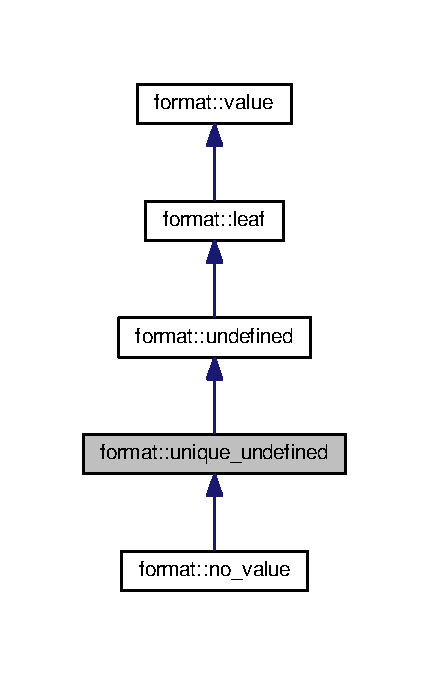
\includegraphics[width=206pt]{classformat_1_1unique__undefined__inherit__graph}
\end{center}
\end{figure}


Collaboration diagram for format\+:\+:unique\+\_\+undefined\+:
\nopagebreak
\begin{figure}[H]
\begin{center}
\leavevmode
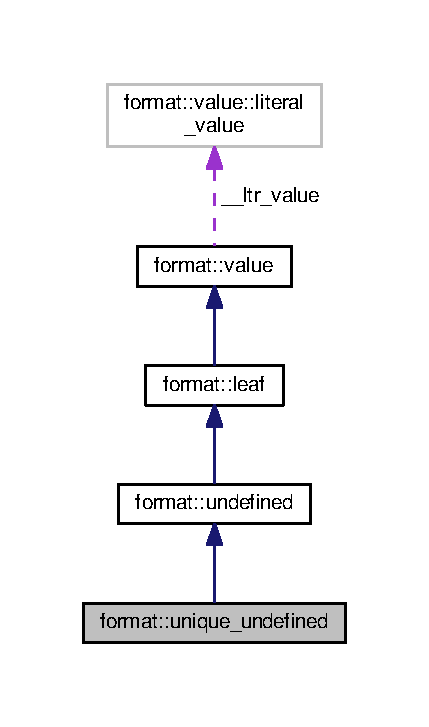
\includegraphics[width=206pt]{classformat_1_1unique__undefined__coll__graph}
\end{center}
\end{figure}
\subsection*{Public Member Functions}
\begin{DoxyCompactItemize}
\item 
\hyperlink{classformat_1_1unique__undefined_afd232b15079ed7da34302cdea4a90677}{unique\+\_\+undefined} ()\hypertarget{classformat_1_1unique__undefined_afd232b15079ed7da34302cdea4a90677}{}\label{classformat_1_1unique__undefined_afd232b15079ed7da34302cdea4a90677}

\begin{DoxyCompactList}\small\item\em \hyperlink{classformat_1_1unique__undefined}{unique\+\_\+undefined} \end{DoxyCompactList}\item 
\hyperlink{classformat_1_1unique__undefined_afba0bc86b45598568a251d38f6a7b731}{unique\+\_\+undefined} (\hyperlink{classformat_1_1json}{json} $\ast$\hyperlink{classformat_1_1value_a86c03ec8810bfd0d60ec49095120040d}{parent})
\begin{DoxyCompactList}\small\item\em \hyperlink{classformat_1_1unique__undefined}{unique\+\_\+undefined} \end{DoxyCompactList}\item 
\hyperlink{classformat_1_1unique__undefined_a6d18209e8bb55eba57c378c84399ea3a}{unique\+\_\+undefined} (const \hyperlink{classformat_1_1unique__undefined}{unique\+\_\+undefined} \&other)=default
\begin{DoxyCompactList}\small\item\em \hyperlink{classformat_1_1unique__undefined}{unique\+\_\+undefined} \end{DoxyCompactList}\item 
virtual \hyperlink{classformat_1_1unique__undefined_a25e675a3f9fc1aab1d19a0f8a05920bf}{$\sim$unique\+\_\+undefined} () override=default\hypertarget{classformat_1_1unique__undefined_a25e675a3f9fc1aab1d19a0f8a05920bf}{}\label{classformat_1_1unique__undefined_a25e675a3f9fc1aab1d19a0f8a05920bf}

\begin{DoxyCompactList}\small\item\em $\sim$unique\+\_\+undefined \end{DoxyCompactList}\item 
virtual \hyperlink{classformat_1_1value_aa6b85823936bf7b8ab78d3f8d443c00d}{value} $\ast$ \hyperlink{classformat_1_1unique__undefined_af69057a00374c21c5cd73dc77efffb0e}{clone} () const 
\begin{DoxyCompactList}\small\item\em clone \end{DoxyCompactList}\item 
void \hyperlink{classformat_1_1unique__undefined_ae15b684d7cce6db1aa0cf71cf6be87c3}{operator delete} (void $\ast$ptr)\hypertarget{classformat_1_1unique__undefined_ae15b684d7cce6db1aa0cf71cf6be87c3}{}\label{classformat_1_1unique__undefined_ae15b684d7cce6db1aa0cf71cf6be87c3}

\begin{DoxyCompactList}\small\item\em operator delete \end{DoxyCompactList}\item 
void \hyperlink{classformat_1_1unique__undefined_a6924635e275064b975384443a67d0579}{operator delete\mbox{[}$\,$\mbox{]}} (void $\ast$ptr)\hypertarget{classformat_1_1unique__undefined_a6924635e275064b975384443a67d0579}{}\label{classformat_1_1unique__undefined_a6924635e275064b975384443a67d0579}

\begin{DoxyCompactList}\small\item\em operator delete\mbox{[}\mbox{]} \end{DoxyCompactList}\end{DoxyCompactItemize}
\subsection*{Static Public Member Functions}
\begin{DoxyCompactItemize}
\item 
static void $\ast$ \hyperlink{classformat_1_1unique__undefined_ab0561911ee891679e009bf3c09aa4ef1}{operator new} (std\+::size\+\_\+t size)
\begin{DoxyCompactList}\small\item\em operator new \end{DoxyCompactList}\item 
static void $\ast$ \hyperlink{classformat_1_1unique__undefined_a89eb80d7eb9e00051bacad091321172c}{operator new\mbox{[}$\,$\mbox{]}} (std\+::size\+\_\+t size)
\begin{DoxyCompactList}\small\item\em operator new\mbox{[}\mbox{]} \end{DoxyCompactList}\end{DoxyCompactItemize}
\subsection*{Additional Inherited Members}


\subsection{Detailed Description}
The \hyperlink{classformat_1_1unique__undefined}{unique\+\_\+undefined} class. 

\subsection{Constructor \& Destructor Documentation}
\index{format\+::unique\+\_\+undefined@{format\+::unique\+\_\+undefined}!unique\+\_\+undefined@{unique\+\_\+undefined}}
\index{unique\+\_\+undefined@{unique\+\_\+undefined}!format\+::unique\+\_\+undefined@{format\+::unique\+\_\+undefined}}
\subsubsection[{\texorpdfstring{unique\+\_\+undefined(json $\ast$parent)}{unique_undefined(json *parent)}}]{\setlength{\rightskip}{0pt plus 5cm}format\+::unique\+\_\+undefined\+::unique\+\_\+undefined (
\begin{DoxyParamCaption}
\item[{{\bf json} $\ast$}]{parent}
\end{DoxyParamCaption}
)\hspace{0.3cm}{\ttfamily [inline]}}\hypertarget{classformat_1_1unique__undefined_afba0bc86b45598568a251d38f6a7b731}{}\label{classformat_1_1unique__undefined_afba0bc86b45598568a251d38f6a7b731}


\hyperlink{classformat_1_1unique__undefined}{unique\+\_\+undefined} 


\begin{DoxyParams}{Parameters}
{\em parent} & \\
\hline
\end{DoxyParams}
\index{format\+::unique\+\_\+undefined@{format\+::unique\+\_\+undefined}!unique\+\_\+undefined@{unique\+\_\+undefined}}
\index{unique\+\_\+undefined@{unique\+\_\+undefined}!format\+::unique\+\_\+undefined@{format\+::unique\+\_\+undefined}}
\subsubsection[{\texorpdfstring{unique\+\_\+undefined(const unique\+\_\+undefined \&other)=default}{unique_undefined(const unique_undefined &other)=default}}]{\setlength{\rightskip}{0pt plus 5cm}format\+::unique\+\_\+undefined\+::unique\+\_\+undefined (
\begin{DoxyParamCaption}
\item[{const {\bf unique\+\_\+undefined} \&}]{other}
\end{DoxyParamCaption}
)\hspace{0.3cm}{\ttfamily [default]}}\hypertarget{classformat_1_1unique__undefined_a6d18209e8bb55eba57c378c84399ea3a}{}\label{classformat_1_1unique__undefined_a6d18209e8bb55eba57c378c84399ea3a}


\hyperlink{classformat_1_1unique__undefined}{unique\+\_\+undefined} 


\begin{DoxyParams}{Parameters}
{\em other} & \\
\hline
\end{DoxyParams}


\subsection{Member Function Documentation}
\index{format\+::unique\+\_\+undefined@{format\+::unique\+\_\+undefined}!clone@{clone}}
\index{clone@{clone}!format\+::unique\+\_\+undefined@{format\+::unique\+\_\+undefined}}
\subsubsection[{\texorpdfstring{clone() const }{clone() const }}]{\setlength{\rightskip}{0pt plus 5cm}virtual {\bf value}$\ast$ format\+::unique\+\_\+undefined\+::clone (
\begin{DoxyParamCaption}
{}
\end{DoxyParamCaption}
) const\hspace{0.3cm}{\ttfamily [inline]}, {\ttfamily [virtual]}}\hypertarget{classformat_1_1unique__undefined_af69057a00374c21c5cd73dc77efffb0e}{}\label{classformat_1_1unique__undefined_af69057a00374c21c5cd73dc77efffb0e}


clone 

\begin{DoxyReturn}{Returns}

\end{DoxyReturn}


Reimplemented from \hyperlink{classformat_1_1undefined_af418bdce70e2d41131ac640fcf6dc121}{format\+::undefined}.

\index{format\+::unique\+\_\+undefined@{format\+::unique\+\_\+undefined}!operator new@{operator new}}
\index{operator new@{operator new}!format\+::unique\+\_\+undefined@{format\+::unique\+\_\+undefined}}
\subsubsection[{\texorpdfstring{operator new(std\+::size\+\_\+t size)}{operator new(std::size_t size)}}]{\setlength{\rightskip}{0pt plus 5cm}static void$\ast$ format\+::unique\+\_\+undefined\+::operator new (
\begin{DoxyParamCaption}
\item[{std\+::size\+\_\+t}]{size}
\end{DoxyParamCaption}
)\hspace{0.3cm}{\ttfamily [inline]}, {\ttfamily [static]}}\hypertarget{classformat_1_1unique__undefined_ab0561911ee891679e009bf3c09aa4ef1}{}\label{classformat_1_1unique__undefined_ab0561911ee891679e009bf3c09aa4ef1}


operator new 


\begin{DoxyParams}{Parameters}
{\em size} & \\
\hline
\end{DoxyParams}
\begin{DoxyReturn}{Returns}

\end{DoxyReturn}
\index{format\+::unique\+\_\+undefined@{format\+::unique\+\_\+undefined}!operator new\mbox{[}$\,$\mbox{]}@{operator new[]}}
\index{operator new\mbox{[}$\,$\mbox{]}@{operator new[]}!format\+::unique\+\_\+undefined@{format\+::unique\+\_\+undefined}}
\subsubsection[{\texorpdfstring{operator new[](std\+::size\+\_\+t size)}{operator new[](std::size_t size)}}]{\setlength{\rightskip}{0pt plus 5cm}static void$\ast$ format\+::unique\+\_\+undefined\+::operator new\mbox{[}$\,$\mbox{]} (
\begin{DoxyParamCaption}
\item[{std\+::size\+\_\+t}]{size}
\end{DoxyParamCaption}
)\hspace{0.3cm}{\ttfamily [inline]}, {\ttfamily [static]}}\hypertarget{classformat_1_1unique__undefined_a89eb80d7eb9e00051bacad091321172c}{}\label{classformat_1_1unique__undefined_a89eb80d7eb9e00051bacad091321172c}


operator new\mbox{[}\mbox{]} 


\begin{DoxyParams}{Parameters}
{\em size} & \\
\hline
\end{DoxyParams}
\begin{DoxyReturn}{Returns}

\end{DoxyReturn}


The documentation for this class was generated from the following file\+:\begin{DoxyCompactItemize}
\item 
json\+\_\+undefined.\+h\end{DoxyCompactItemize}

\hypertarget{classformat_1_1value}{}\section{format\+:\+:value Class Reference}
\label{classformat_1_1value}\index{format\+::value@{format\+::value}}


Inheritance diagram for format\+:\+:value\+:
\nopagebreak
\begin{figure}[H]
\begin{center}
\leavevmode
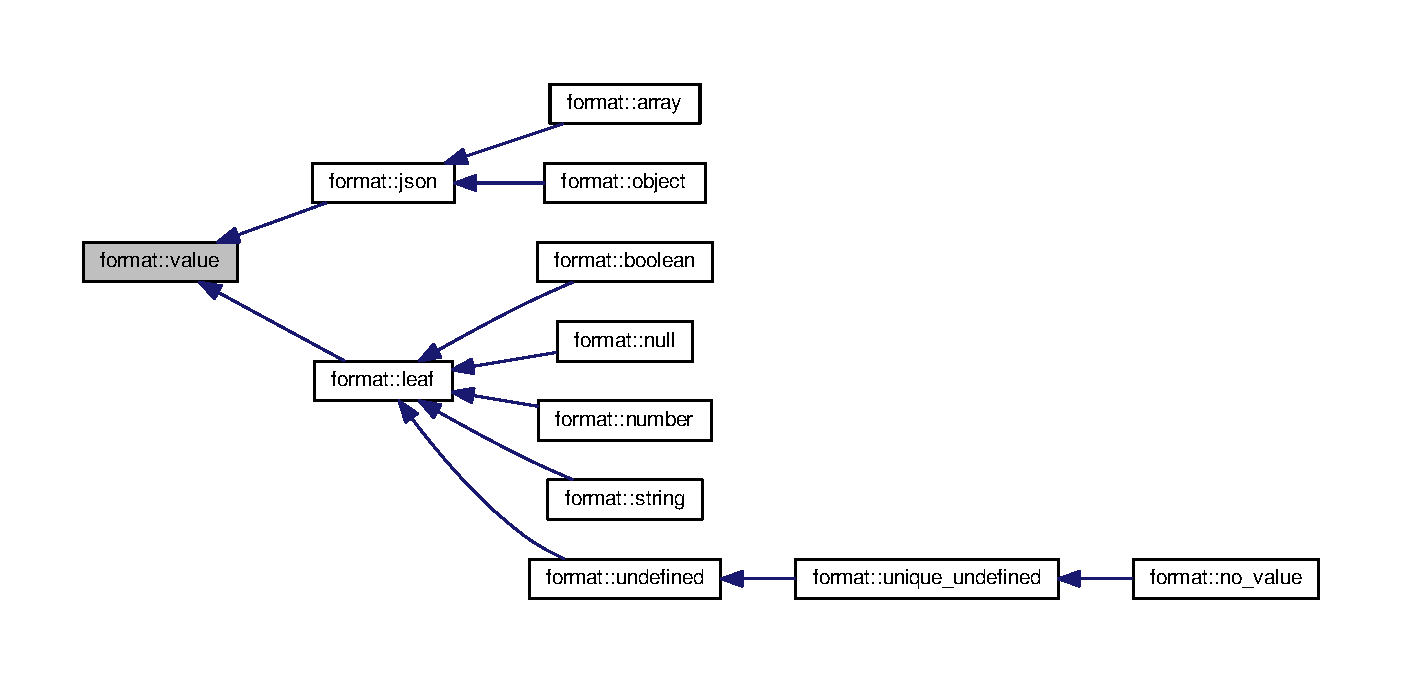
\includegraphics[width=350pt]{classformat_1_1value__inherit__graph}
\end{center}
\end{figure}


Collaboration diagram for format\+:\+:value\+:
\nopagebreak
\begin{figure}[H]
\begin{center}
\leavevmode
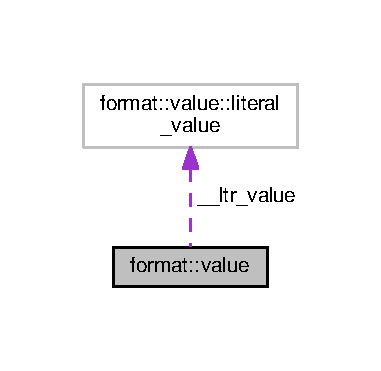
\includegraphics[width=183pt]{classformat_1_1value__coll__graph}
\end{center}
\end{figure}
\subsection*{Classes}
\begin{DoxyCompactItemize}
\item 
class \hyperlink{classformat_1_1value_1_1iterator}{iterator}
\begin{DoxyCompactList}\small\item\em The iterator class. \end{DoxyCompactList}\item 
struct {\bfseries literal\+\_\+value}
\begin{DoxyCompactList}\small\item\em \+\_\+literal\+\_\+value \end{DoxyCompactList}\end{DoxyCompactItemize}
\subsection*{Public Types}
\begin{DoxyCompactItemize}
\item 
enum \hyperlink{classformat_1_1value_aa0334be06389a7b14af485fa0cd3aa21}{value\+\_\+t} \{ \\*
{\bfseries no\+\_\+value\+\_\+t} = 0, 
{\bfseries undefined\+\_\+t}, 
{\bfseries object\+\_\+t}, 
{\bfseries array\+\_\+t}, 
\\*
{\bfseries string\+\_\+t}, 
{\bfseries number\+\_\+t}, 
{\bfseries boolean\+\_\+t}, 
{\bfseries null\+\_\+t}
 \}\hypertarget{classformat_1_1value_aa0334be06389a7b14af485fa0cd3aa21}{}\label{classformat_1_1value_aa0334be06389a7b14af485fa0cd3aa21}
\begin{DoxyCompactList}\small\item\em The otype enum. \end{DoxyCompactList}
\end{DoxyCompactItemize}
\subsection*{Public Member Functions}
\begin{DoxyCompactItemize}
\item 
\hyperlink{classformat_1_1value_aa6b85823936bf7b8ab78d3f8d443c00d}{value} ()\hypertarget{classformat_1_1value_aa6b85823936bf7b8ab78d3f8d443c00d}{}\label{classformat_1_1value_aa6b85823936bf7b8ab78d3f8d443c00d}

\begin{DoxyCompactList}\small\item\em Value. \end{DoxyCompactList}\item 
\hyperlink{classformat_1_1value_a3c21663a87408a066b93bc41a099f1d8}{value} (const wchar\+\_\+t $\ast$)
\begin{DoxyCompactList}\small\item\em json\+\_\+value \end{DoxyCompactList}\item 
\hyperlink{classformat_1_1value_a6519ed65370e658a185a0a0db0152554}{value} (const \hyperlink{classformat_1_1value}{value} \&other)
\begin{DoxyCompactList}\small\item\em value \end{DoxyCompactList}\item 
virtual \hyperlink{classformat_1_1value}{value} $\ast$ \hyperlink{classformat_1_1value_a8756eb79e41851859d83ae46069dc400}{clone} () const =0
\begin{DoxyCompactList}\small\item\em clone Call object copy constructor when derived type in not known \end{DoxyCompactList}\item 
virtual \hyperlink{classformat_1_1value_a909766075c9375317ef5e842741f666d}{$\sim$value} ()\hypertarget{classformat_1_1value_a909766075c9375317ef5e842741f666d}{}\label{classformat_1_1value_a909766075c9375317ef5e842741f666d}

\begin{DoxyCompactList}\small\item\em $\sim$\+Value \end{DoxyCompactList}\item 
\hyperlink{classformat_1_1value}{value} \& \hyperlink{classformat_1_1value_a59a729393bc6137e6782ea96f89bf18a}{operator\mbox{[}$\,$\mbox{]}} (const wchar\+\_\+t $\ast$\hyperlink{classformat_1_1value_ad4865e7984fc9f3b5ce7c17fd7ac740c}{key})
\begin{DoxyCompactList}\small\item\em operator \mbox{[}\mbox{]} \end{DoxyCompactList}\item 
\hyperlink{classformat_1_1value}{value} \& \hyperlink{classformat_1_1value_a68e009d6421f7a127978e9b48adcf200}{operator\mbox{[}$\,$\mbox{]}} (size\+\_\+t \hyperlink{classformat_1_1value_aaa429b28cc0edf5a3589b89a1820ad62}{index})
\begin{DoxyCompactList}\small\item\em operator \mbox{[}\mbox{]} \end{DoxyCompactList}\item 
\hyperlink{classformat_1_1value}{value} \& \hyperlink{classformat_1_1value_aae4cf62ca68a4df00a31a66c1c576c3e}{operator=} (\hyperlink{classformat_1_1value}{value} $\ast$v)
\begin{DoxyCompactList}\small\item\em operator = \end{DoxyCompactList}\item 
\hyperlink{classformat_1_1value}{value} \& \hyperlink{classformat_1_1value_a711e2949ae310096a9e429c52574fffc}{operator=} (const \hyperlink{classformat_1_1value}{value} \&v)
\begin{DoxyCompactList}\small\item\em operator = \end{DoxyCompactList}\item 
\hyperlink{classformat_1_1value}{value} \& \hyperlink{classformat_1_1value_a126201c87fd63a093fecc2e16735ac52}{operator=} (const undefined \&u)
\begin{DoxyCompactList}\small\item\em operator = \end{DoxyCompactList}\item 
\hyperlink{classformat_1_1value}{value} \& \hyperlink{classformat_1_1value_a0a17ba9f3d99be0c1d86d91adac0bb60}{operator=} (const wchar\+\_\+t $\ast$json\+\_\+text)
\begin{DoxyCompactList}\small\item\em operator = \end{DoxyCompactList}\item 
\hyperlink{classformat_1_1value}{value} \& \hyperlink{classformat_1_1value_a1636e6762c97584eb15b85b6a6422055}{operator=} (double d)
\begin{DoxyCompactList}\small\item\em operator = \end{DoxyCompactList}\item 
\hyperlink{classformat_1_1value}{value} \& \hyperlink{classformat_1_1value_a017ba8a51e1005652ab3113c6b0951ec}{operator=} (bool b)
\begin{DoxyCompactList}\small\item\em operator = \end{DoxyCompactList}\item 
\hyperlink{classformat_1_1value}{value} \& \hyperlink{classformat_1_1value_a0c62128d9917513e97068a267b4543ca}{operator=} (std\+::nullptr\+\_\+t)
\begin{DoxyCompactList}\small\item\em operator = \end{DoxyCompactList}\item 
virtual \hyperlink{classformat_1_1value_aa0334be06389a7b14af485fa0cd3aa21}{value\+\_\+t} \hyperlink{classformat_1_1value_a7112d0f83cf61aa9e1cdde90fc444996}{type} () const noexcept=0
\begin{DoxyCompactList}\small\item\em type \end{DoxyCompactList}\item 
bool \hyperlink{classformat_1_1value_a3bd4d42103322d1c6940e04554405a8e}{operator==} (\hyperlink{classformat_1_1value_aa0334be06389a7b14af485fa0cd3aa21}{value\+\_\+t} t) const noexcept
\begin{DoxyCompactList}\small\item\em operator == \end{DoxyCompactList}\item 
bool \hyperlink{classformat_1_1value_ad18cb4b5aef50630f5fab8a6d52816b7}{operator==} (const \hyperlink{classformat_1_1value}{value} \&v) const noexcept
\begin{DoxyCompactList}\small\item\em operator == \end{DoxyCompactList}\item 
virtual size\+\_\+t \hyperlink{classformat_1_1value_a406a9553c4d83a0613aa54d77f6c462d}{length} () const noexcept=0
\begin{DoxyCompactList}\small\item\em count \end{DoxyCompactList}\item 
const wchar\+\_\+t $\ast$ \hyperlink{classformat_1_1value_ad4865e7984fc9f3b5ce7c17fd7ac740c}{key} () const noexcept
\begin{DoxyCompactList}\small\item\em key \end{DoxyCompactList}\item 
size\+\_\+t \hyperlink{classformat_1_1value_aaa429b28cc0edf5a3589b89a1820ad62}{index} () const noexcept
\begin{DoxyCompactList}\small\item\em index \end{DoxyCompactList}\item 
const wchar\+\_\+t $\ast$ \hyperlink{classformat_1_1value_a7fb73377471f5ed99695846340130348}{stringify} () noexcept
\begin{DoxyCompactList}\small\item\em stringify \end{DoxyCompactList}\item 
virtual size\+\_\+t \hyperlink{classformat_1_1value_a399280e27e629db0582b5781b90ca58b}{str\+\_\+length} () const noexcept=0
\begin{DoxyCompactList}\small\item\em str\+\_\+length \end{DoxyCompactList}\item 
const wchar\+\_\+t $\ast$ \hyperlink{classformat_1_1value_af89058b38ae886a02713b5a556f7fe17}{get} () const 
\begin{DoxyCompactList}\small\item\em value \end{DoxyCompactList}\item 
json $\ast$ \hyperlink{classformat_1_1value_a86c03ec8810bfd0d60ec49095120040d}{parent} () const 
\begin{DoxyCompactList}\small\item\em parent \end{DoxyCompactList}\end{DoxyCompactItemize}
\subsection*{Protected Types}
\begin{DoxyCompactItemize}
\item 
enum \hyperlink{classformat_1_1value_a048b1ae29385f7eb708899eebddd1e59}{\+\_\+sc} \{ \\*
{\bfseries begin\+\_\+object} = \textquotesingle{}\{\textquotesingle{}, 
{\bfseries end\+\_\+object} = \textquotesingle{}\}\textquotesingle{}, 
{\bfseries begin\+\_\+array} = \textquotesingle{}\mbox{[}\textquotesingle{}, 
{\bfseries end\+\_\+array} = \textquotesingle{}\mbox{]}\textquotesingle{}, 
\\*
{\bfseries name\+\_\+separator} = \textquotesingle{}\+:\textquotesingle{}, 
{\bfseries value\+\_\+separator} = \textquotesingle{},\textquotesingle{}, 
{\bfseries double\+\_\+quote} = 34
 \}\hypertarget{classformat_1_1value_a048b1ae29385f7eb708899eebddd1e59}{}\label{classformat_1_1value_a048b1ae29385f7eb708899eebddd1e59}
\begin{DoxyCompactList}\small\item\em The \+\_\+sc enum Structural characters. \end{DoxyCompactList}
\item 
enum \hyperlink{classformat_1_1value_a6720d6d39ff203499cfd97747487320b}{\+\_\+ws} \{ {\bfseries tab} = 9, 
{\bfseries lf} = 10, 
{\bfseries cr} = 13, 
{\bfseries space} = 32
 \}\hypertarget{classformat_1_1value_a6720d6d39ff203499cfd97747487320b}{}\label{classformat_1_1value_a6720d6d39ff203499cfd97747487320b}
\begin{DoxyCompactList}\small\item\em The \+\_\+ws enum White space characters. \end{DoxyCompactList}
\item 
enum \hyperlink{classformat_1_1value_a953390030c22a816b7c9b2b54d4992a8}{\+\_\+literal} \{ {\bfseries no\+\_\+literal} = 0, 
{\bfseries true\+\_\+value} = 1, 
{\bfseries false\+\_\+value} = 2, 
{\bfseries null\+\_\+value} = 3
 \}\hypertarget{classformat_1_1value_a953390030c22a816b7c9b2b54d4992a8}{}\label{classformat_1_1value_a953390030c22a816b7c9b2b54d4992a8}
\begin{DoxyCompactList}\small\item\em The literal enum. \end{DoxyCompactList}
\end{DoxyCompactItemize}
\subsection*{Protected Member Functions}
\begin{DoxyCompactItemize}
\item 
virtual const wchar\+\_\+t $\ast$ \hyperlink{classformat_1_1value_a7859b1aa48f667a83e091f0eba22d4a1}{\+\_\+parse} (const wchar\+\_\+t $\ast$json)=0
\begin{DoxyCompactList}\small\item\em \+\_\+parse \end{DoxyCompactList}\item 
\hyperlink{classformat_1_1value}{value} \& \hyperlink{classformat_1_1value_ab791aabbee3a4a415a62910c150b0a82}{\+\_\+assign} (\hyperlink{classformat_1_1value}{value} $\ast$nv)
\begin{DoxyCompactList}\small\item\em \+\_\+assign \end{DoxyCompactList}\item 
\hyperlink{classformat_1_1value}{value} \& \hyperlink{classformat_1_1value_a0e07a062f2925491a1a148cc77ae2e86}{\+\_\+assign} (const \hyperlink{classformat_1_1value}{value} \&nv)
\begin{DoxyCompactList}\small\item\em assign \end{DoxyCompactList}\item 
virtual \hyperlink{classformat_1_1value}{value} \& \hyperlink{classformat_1_1value_a2432012e597ef7a5c853c184c77f8310}{\+\_\+assign} (\hyperlink{classformat_1_1value}{value} $\ast$, \hyperlink{classformat_1_1value}{value} $\ast$)=0
\begin{DoxyCompactList}\small\item\em \+\_\+assign \end{DoxyCompactList}\item 
\hyperlink{classformat_1_1value}{value} \& \hyperlink{classformat_1_1value_adf5e3905bcb7b8616981831de01e3555}{\+\_\+assign} (const undefined \&) noexcept
\begin{DoxyCompactList}\small\item\em \+\_\+assign \end{DoxyCompactList}\item 
void \hyperlink{classformat_1_1value_a473256bcee74e255df322920d250aac0}{\+\_\+set\+\_\+key} (const wchar\+\_\+t $\ast$\hyperlink{classformat_1_1value_ad4865e7984fc9f3b5ce7c17fd7ac740c}{key}, size\+\_\+t charc) noexcept
\begin{DoxyCompactList}\small\item\em \+\_\+set\+\_\+key \end{DoxyCompactList}\item 
void \hyperlink{classformat_1_1value_a6b16897991f5e9166924d644b213dad6}{\+\_\+set\+\_\+index} (const size\+\_\+t \&\hyperlink{classformat_1_1value_aaa429b28cc0edf5a3589b89a1820ad62}{index}) noexcept
\begin{DoxyCompactList}\small\item\em \+\_\+set\+\_\+index \end{DoxyCompactList}\item 
void \hyperlink{classformat_1_1value_a1be7f20ce6fd552089771422dc28b695}{\+\_\+set\+\_\+parent} (json $\ast$\hyperlink{classformat_1_1value_a86c03ec8810bfd0d60ec49095120040d}{parent}) noexcept
\begin{DoxyCompactList}\small\item\em set\+Parent \end{DoxyCompactList}\item 
\hyperlink{classformat_1_1value_a2d4230f4fa939f6f5c451dbebc7fffba}{value} (json $\ast$\hyperlink{classformat_1_1value_a86c03ec8810bfd0d60ec49095120040d}{parent})
\begin{DoxyCompactList}\small\item\em value \end{DoxyCompactList}\item 
virtual const wchar\+\_\+t $\ast$ \hyperlink{classformat_1_1value_a94ed31f07b19866495297472accd33a8}{\+\_\+to\+\_\+string} (wchar\+\_\+t $\ast$offset=0) const =0
\begin{DoxyCompactList}\small\item\em str\+\_\+value \end{DoxyCompactList}\item 
virtual \hyperlink{classformat_1_1value}{value} $\ast$ \hyperlink{classformat_1_1value_a5d0a94cbdaf98d5420c5d55bd4345663}{\+\_\+clone} (const \hyperlink{classformat_1_1value}{value} \&other)=0
\begin{DoxyCompactList}\small\item\em \+\_\+clone Called by copy constructor \end{DoxyCompactList}\item 
const wchar\+\_\+t $\ast$ \hyperlink{classformat_1_1value_aea0aec2d465431ca45d20ff0a18f6ea6}{\+\_\+look\+\_\+ahead} () noexcept\hypertarget{classformat_1_1value_aea0aec2d465431ca45d20ff0a18f6ea6}{}\label{classformat_1_1value_aea0aec2d465431ca45d20ff0a18f6ea6}

\begin{DoxyCompactList}\small\item\em \+\_\+look\+\_\+ahead Move read pointer to next non-\/white space character \end{DoxyCompactList}\item 
long int \hyperlink{classformat_1_1value_aab0e0227afa4e70d382608b4d75a9140}{\+\_\+string} (wchar\+\_\+t \&endc) const noexcept
\begin{DoxyCompactList}\small\item\em \+\_\+string Read in string. If no opening quote, return 0. If no closing quote or unescaped unicode control character (0-\/31) met, return number characters read as a negative value. For example \char`\"{}\textbackslash{}\char`\"{}xx"\char`\"{} = -\/3
\+Else return number of characters read + 2 (quotes). For example \char`\"{}"xxx"" = 5 \end{DoxyCompactList}\item 
\hyperlink{classformat_1_1value_a953390030c22a816b7c9b2b54d4992a8}{value\+::\+\_\+literal} \hyperlink{classformat_1_1value_ada2428d6e7f55e46096912fdec16a17d}{\+\_\+is\+\_\+literal} (const int \+\_\+try=0) const noexcept
\begin{DoxyCompactList}\small\item\em \+\_\+is\+\_\+literal Detect if \+\_\+readp points to \char`\"{}true\char`\"{}, \char`\"{}false\char`\"{} or \char`\"{}null\char`\"{}. \end{DoxyCompactList}\item 
virtual \hyperlink{classformat_1_1value}{value} \& \hyperlink{classformat_1_1value_a3f67662acb201f2ab8a768f8cb670678}{\+\_\+at} (const wchar\+\_\+t $\ast$\hyperlink{classformat_1_1value_ad4865e7984fc9f3b5ce7c17fd7ac740c}{key})=0
\begin{DoxyCompactList}\small\item\em \+\_\+at json\+::object behavior\+: if key does not exist, assign key with value of type undefined. \end{DoxyCompactList}\item 
virtual \hyperlink{classformat_1_1value}{value} \& \hyperlink{classformat_1_1value_ab94a7f0af8ea5c60fd0e59ccde8d0371}{\+\_\+at} (size\+\_\+t \hyperlink{classformat_1_1value_aaa429b28cc0edf5a3589b89a1820ad62}{index})=0
\begin{DoxyCompactList}\small\item\em \+\_\+at \end{DoxyCompactList}\item 
virtual void \hyperlink{classformat_1_1value_a9924ec6809a88b2fc59b1be7a4835127}{\+\_\+clear} ()=0\hypertarget{classformat_1_1value_a9924ec6809a88b2fc59b1be7a4835127}{}\label{classformat_1_1value_a9924ec6809a88b2fc59b1be7a4835127}

\begin{DoxyCompactList}\small\item\em \+\_\+clear \end{DoxyCompactList}\item 
virtual \hyperlink{classformat_1_1value}{value} \& \hyperlink{classformat_1_1value_a75537c78ab53ac7657eea750b94259b3}{\+\_\+erase} (const \hyperlink{classformat_1_1value}{value} \&v) noexcept=0
\begin{DoxyCompactList}\small\item\em \+\_\+erase \end{DoxyCompactList}\end{DoxyCompactItemize}
\subsection*{Static Protected Member Functions}
\begin{DoxyCompactItemize}
\item 
static wchar\+\_\+t $\ast$ \hyperlink{classformat_1_1value_a5d029f82ccef1f9df32f617baf32e41d}{\+\_\+str\+\_\+append} (wchar\+\_\+t $\ast$dst, const wchar\+\_\+t $\ast$src, size\+\_\+t charc) noexcept
\begin{DoxyCompactList}\small\item\em \+\_\+str\+\_\+append Copy src to dst. Move dst right after the last copied character. \end{DoxyCompactList}\end{DoxyCompactItemize}
\subsection*{Protected Attributes}
\begin{DoxyCompactItemize}
\item 
const wchar\+\_\+t $\ast$ \hyperlink{classformat_1_1value_a1bbc05a0a601228e7282dc748cbe3d01}{\+\_\+readp}\hypertarget{classformat_1_1value_a1bbc05a0a601228e7282dc748cbe3d01}{}\label{classformat_1_1value_a1bbc05a0a601228e7282dc748cbe3d01}

\begin{DoxyCompactList}\small\item\em \+\_\+readp \end{DoxyCompactList}\item 
json $\ast$ \hyperlink{classformat_1_1value_a933c180828081a6b7582fca1b268b389}{\+\_\+parent}\hypertarget{classformat_1_1value_a933c180828081a6b7582fca1b268b389}{}\label{classformat_1_1value_a933c180828081a6b7582fca1b268b389}

\begin{DoxyCompactList}\small\item\em \+\_\+parent \end{DoxyCompactList}\item 
const wchar\+\_\+t $\ast$ \hyperlink{classformat_1_1value_af4f315a1f5b893f57b533117102938dd}{\+\_\+key}\hypertarget{classformat_1_1value_af4f315a1f5b893f57b533117102938dd}{}\label{classformat_1_1value_af4f315a1f5b893f57b533117102938dd}

\begin{DoxyCompactList}\small\item\em \+\_\+key \end{DoxyCompactList}\item 
size\+\_\+t \hyperlink{classformat_1_1value_af86a1855af003b54881a284a99463f37}{\+\_\+index}\hypertarget{classformat_1_1value_af86a1855af003b54881a284a99463f37}{}\label{classformat_1_1value_af86a1855af003b54881a284a99463f37}

\begin{DoxyCompactList}\small\item\em \+\_\+index \end{DoxyCompactList}\end{DoxyCompactItemize}
\subsection*{Static Protected Attributes}
\begin{DoxyCompactItemize}
\item 
static const struct format\+::value\+::literal\+\_\+value {\bfseries \+\_\+\+\_\+ltr\+\_\+value} \mbox{[}3\mbox{]}\hypertarget{classformat_1_1value_afb89a1ddf5bf430f6fe26adc263abe2d}{}\label{classformat_1_1value_afb89a1ddf5bf430f6fe26adc263abe2d}

\end{DoxyCompactItemize}
\subsection*{Friends}
\begin{DoxyCompactItemize}
\item 
const wchar\+\_\+t $\ast$ {\bfseries \+\_\+\+\_\+call\+\_\+\+\_\+parse} (\hyperlink{classformat_1_1value}{value} $\ast$, const wchar\+\_\+t $\ast$)\hypertarget{classformat_1_1value_a91e0ce1b19bc26c2887f0321e7c5c2e8}{}\label{classformat_1_1value_a91e0ce1b19bc26c2887f0321e7c5c2e8}

\item 
void {\bfseries \+\_\+\+\_\+call\+\_\+\+\_\+set\+\_\+key} (\hyperlink{classformat_1_1value}{value} $\ast$, const wchar\+\_\+t $\ast$, size\+\_\+t)\hypertarget{classformat_1_1value_a1891a795b58e455d457f20cc5b36705f}{}\label{classformat_1_1value_a1891a795b58e455d457f20cc5b36705f}

\item 
void {\bfseries \+\_\+\+\_\+call\+\_\+\+\_\+set\+\_\+index} (\hyperlink{classformat_1_1value}{value} $\ast$, const size\+\_\+t \&)\hypertarget{classformat_1_1value_a0a25629ae14bd56c2583fe7b7a2e9397}{}\label{classformat_1_1value_a0a25629ae14bd56c2583fe7b7a2e9397}

\item 
void {\bfseries \+\_\+\+\_\+call\+\_\+\+\_\+set\+\_\+parent} (\hyperlink{classformat_1_1value}{value} $\ast$, json $\ast$)\hypertarget{classformat_1_1value_a43fc53d952c0f7fa94f2926bbc7700f2}{}\label{classformat_1_1value_a43fc53d952c0f7fa94f2926bbc7700f2}

\item 
const wchar\+\_\+t $\ast$ {\bfseries \+\_\+\+\_\+call\+\_\+str\+\_\+value} (\hyperlink{classformat_1_1value}{value} $\ast$, wchar\+\_\+t $\ast$)\hypertarget{classformat_1_1value_a7c14f855473e8ae2783404baaeb77ef3}{}\label{classformat_1_1value_a7c14f855473e8ae2783404baaeb77ef3}

\item 
\hyperlink{classformat_1_1value}{value} \& {\bfseries \+\_\+\+\_\+call\+\_\+\+\_\+erase} (\hyperlink{classformat_1_1value}{value} $\ast$, const \hyperlink{classformat_1_1value}{value} \&)\hypertarget{classformat_1_1value_adeaa91cfb33848f060cc7ebccd228ecb}{}\label{classformat_1_1value_adeaa91cfb33848f060cc7ebccd228ecb}

\end{DoxyCompactItemize}


\subsection{Constructor \& Destructor Documentation}
\index{format\+::value@{format\+::value}!value@{value}}
\index{value@{value}!format\+::value@{format\+::value}}
\subsubsection[{\texorpdfstring{value(const wchar\+\_\+t $\ast$)}{value(const wchar_t *)}}]{\setlength{\rightskip}{0pt plus 5cm}format\+::value\+::value (
\begin{DoxyParamCaption}
\item[{const wchar\+\_\+t $\ast$}]{}
\end{DoxyParamCaption}
)}\hypertarget{classformat_1_1value_a3c21663a87408a066b93bc41a099f1d8}{}\label{classformat_1_1value_a3c21663a87408a066b93bc41a099f1d8}


json\+\_\+value 


\begin{DoxyParams}{Parameters}
{\em json} & \\
\hline
\end{DoxyParams}
\index{format\+::value@{format\+::value}!value@{value}}
\index{value@{value}!format\+::value@{format\+::value}}
\subsubsection[{\texorpdfstring{value(const value \&other)}{value(const value &other)}}]{\setlength{\rightskip}{0pt plus 5cm}format\+::value\+::value (
\begin{DoxyParamCaption}
\item[{const {\bf value} \&}]{other}
\end{DoxyParamCaption}
)}\hypertarget{classformat_1_1value_a6519ed65370e658a185a0a0db0152554}{}\label{classformat_1_1value_a6519ed65370e658a185a0a0db0152554}


value 


\begin{DoxyParams}{Parameters}
{\em d} & value \\
\hline
{\em b} & value \\
\hline
{\em Value} & \\
\hline
{\em other} & \\
\hline
\end{DoxyParams}
\index{format\+::value@{format\+::value}!value@{value}}
\index{value@{value}!format\+::value@{format\+::value}}
\subsubsection[{\texorpdfstring{value(json $\ast$parent)}{value(json *parent)}}]{\setlength{\rightskip}{0pt plus 5cm}format\+::value\+::value (
\begin{DoxyParamCaption}
\item[{json $\ast$}]{parent}
\end{DoxyParamCaption}
)\hspace{0.3cm}{\ttfamily [protected]}}\hypertarget{classformat_1_1value_a2d4230f4fa939f6f5c451dbebc7fffba}{}\label{classformat_1_1value_a2d4230f4fa939f6f5c451dbebc7fffba}


value 


\begin{DoxyParams}{Parameters}
{\em parent} & \\
\hline
\end{DoxyParams}


\subsection{Member Function Documentation}
\index{format\+::value@{format\+::value}!\+\_\+assign@{\+\_\+assign}}
\index{\+\_\+assign@{\+\_\+assign}!format\+::value@{format\+::value}}
\subsubsection[{\texorpdfstring{\+\_\+assign(value $\ast$nv)}{_assign(value *nv)}}]{\setlength{\rightskip}{0pt plus 5cm}{\bf format\+::value} \& format\+::value\+::\+\_\+assign (
\begin{DoxyParamCaption}
\item[{{\bf value} $\ast$}]{nv}
\end{DoxyParamCaption}
)\hspace{0.3cm}{\ttfamily [protected]}}\hypertarget{classformat_1_1value_ab791aabbee3a4a415a62910c150b0a82}{}\label{classformat_1_1value_ab791aabbee3a4a415a62910c150b0a82}


\+\_\+assign 


\begin{DoxyParams}{Parameters}
{\em nv} & \\
\hline
\end{DoxyParams}
\begin{DoxyReturn}{Returns}

\end{DoxyReturn}
\index{format\+::value@{format\+::value}!\+\_\+assign@{\+\_\+assign}}
\index{\+\_\+assign@{\+\_\+assign}!format\+::value@{format\+::value}}
\subsubsection[{\texorpdfstring{\+\_\+assign(const value \&nv)}{_assign(const value &nv)}}]{\setlength{\rightskip}{0pt plus 5cm}{\bf format\+::value} \& format\+::value\+::\+\_\+assign (
\begin{DoxyParamCaption}
\item[{const {\bf value} \&}]{nv}
\end{DoxyParamCaption}
)\hspace{0.3cm}{\ttfamily [protected]}}\hypertarget{classformat_1_1value_a0e07a062f2925491a1a148cc77ae2e86}{}\label{classformat_1_1value_a0e07a062f2925491a1a148cc77ae2e86}


assign 

If value has parent object, assign to new value to this-\/$>$\+\_\+parent-\/$>$\mbox{[}key\mbox{]}, otherwise assign new value to Value object itself.


\begin{DoxyParams}{Parameters}
{\em nv} & \\
\hline
\end{DoxyParams}
\begin{DoxyReturn}{Returns}

\end{DoxyReturn}
\index{format\+::value@{format\+::value}!\+\_\+assign@{\+\_\+assign}}
\index{\+\_\+assign@{\+\_\+assign}!format\+::value@{format\+::value}}
\subsubsection[{\texorpdfstring{\+\_\+assign(value $\ast$, value $\ast$)=0}{_assign(value *, value *)=0}}]{\setlength{\rightskip}{0pt plus 5cm}virtual {\bf value}\& format\+::value\+::\+\_\+assign (
\begin{DoxyParamCaption}
\item[{{\bf value} $\ast$}]{, }
\item[{{\bf value} $\ast$}]{}
\end{DoxyParamCaption}
)\hspace{0.3cm}{\ttfamily [protected]}, {\ttfamily [pure virtual]}}\hypertarget{classformat_1_1value_a2432012e597ef7a5c853c184c77f8310}{}\label{classformat_1_1value_a2432012e597ef7a5c853c184c77f8310}


\+\_\+assign 

Assign Value object to member\+\_\+list or element\+\_\+list.


\begin{DoxyParams}{Parameters}
{\em Old} & value \\
\hline
{\em New} & value \\
\hline
\end{DoxyParams}
\begin{DoxyReturn}{Returns}

\end{DoxyReturn}
\index{format\+::value@{format\+::value}!\+\_\+assign@{\+\_\+assign}}
\index{\+\_\+assign@{\+\_\+assign}!format\+::value@{format\+::value}}
\subsubsection[{\texorpdfstring{\+\_\+assign(const undefined \&) noexcept}{_assign(const undefined &) noexcept}}]{\setlength{\rightskip}{0pt plus 5cm}{\bf format\+::value} \& format\+::value\+::\+\_\+assign (
\begin{DoxyParamCaption}
\item[{const undefined \&}]{}
\end{DoxyParamCaption}
)\hspace{0.3cm}{\ttfamily [protected]}, {\ttfamily [noexcept]}}\hypertarget{classformat_1_1value_adf5e3905bcb7b8616981831de01e3555}{}\label{classformat_1_1value_adf5e3905bcb7b8616981831de01e3555}


\+\_\+assign 

If value has parent object, remove value from it\textquotesingle{}s parent, otherwise do nothing.


\begin{DoxyParams}{Parameters}
{\em u} & \\
\hline
\end{DoxyParams}
\begin{DoxyReturn}{Returns}

\end{DoxyReturn}
\index{format\+::value@{format\+::value}!\+\_\+at@{\+\_\+at}}
\index{\+\_\+at@{\+\_\+at}!format\+::value@{format\+::value}}
\subsubsection[{\texorpdfstring{\+\_\+at(const wchar\+\_\+t $\ast$key)=0}{_at(const wchar_t *key)=0}}]{\setlength{\rightskip}{0pt plus 5cm}virtual {\bf value}\& format\+::value\+::\+\_\+at (
\begin{DoxyParamCaption}
\item[{const wchar\+\_\+t $\ast$}]{key}
\end{DoxyParamCaption}
)\hspace{0.3cm}{\ttfamily [protected]}, {\ttfamily [pure virtual]}}\hypertarget{classformat_1_1value_a3f67662acb201f2ab8a768f8cb670678}{}\label{classformat_1_1value_a3f67662acb201f2ab8a768f8cb670678}


\+\_\+at json\+::object behavior\+: if key does not exist, assign key with value of type undefined. 


\begin{DoxyParams}{Parameters}
{\em key} & \\
\hline
\end{DoxyParams}
\begin{DoxyReturn}{Returns}

\end{DoxyReturn}


Implemented in \hyperlink{classformat_1_1object_a91e3027c7786c2e24ca3e001f648542d}{format\+::object}, \hyperlink{classformat_1_1array_a6e6822294f55273f657732d048aa38f8}{format\+::array}, \hyperlink{classformat_1_1json_afcb78dfb597d7d609c66a4d5b6575082}{format\+::json}, and \hyperlink{classformat_1_1leaf_aa92aad1668dce02132ca0920b8803f1f}{format\+::leaf}.

\index{format\+::value@{format\+::value}!\+\_\+at@{\+\_\+at}}
\index{\+\_\+at@{\+\_\+at}!format\+::value@{format\+::value}}
\subsubsection[{\texorpdfstring{\+\_\+at(size\+\_\+t index)=0}{_at(size_t index)=0}}]{\setlength{\rightskip}{0pt plus 5cm}virtual {\bf value}\& format\+::value\+::\+\_\+at (
\begin{DoxyParamCaption}
\item[{size\+\_\+t}]{index}
\end{DoxyParamCaption}
)\hspace{0.3cm}{\ttfamily [protected]}, {\ttfamily [pure virtual]}}\hypertarget{classformat_1_1value_ab94a7f0af8ea5c60fd0e59ccde8d0371}{}\label{classformat_1_1value_ab94a7f0af8ea5c60fd0e59ccde8d0371}


\+\_\+at 


\begin{DoxyParams}{Parameters}
{\em index} & \\
\hline
\end{DoxyParams}
\begin{DoxyReturn}{Returns}

\end{DoxyReturn}


Implemented in \hyperlink{classformat_1_1object_a525bdfa2db22cd6bc21a868a695fe752}{format\+::object}, \hyperlink{classformat_1_1array_a386fd4c0f2556459186db7f22df4128e}{format\+::array}, \hyperlink{classformat_1_1json_a4a3924d5a112cda2bcee45ddf92a3d52}{format\+::json}, and \hyperlink{classformat_1_1leaf_a629bf52297b80f099b6477ff88761a2b}{format\+::leaf}.

\index{format\+::value@{format\+::value}!\+\_\+clone@{\+\_\+clone}}
\index{\+\_\+clone@{\+\_\+clone}!format\+::value@{format\+::value}}
\subsubsection[{\texorpdfstring{\+\_\+clone(const value \&other)=0}{_clone(const value &other)=0}}]{\setlength{\rightskip}{0pt plus 5cm}virtual {\bf value}$\ast$ format\+::value\+::\+\_\+clone (
\begin{DoxyParamCaption}
\item[{const {\bf value} \&}]{other}
\end{DoxyParamCaption}
)\hspace{0.3cm}{\ttfamily [protected]}, {\ttfamily [pure virtual]}}\hypertarget{classformat_1_1value_a5d0a94cbdaf98d5420c5d55bd4345663}{}\label{classformat_1_1value_a5d0a94cbdaf98d5420c5d55bd4345663}


\+\_\+clone Called by copy constructor 


\begin{DoxyParams}{Parameters}
{\em other} & \\
\hline
\end{DoxyParams}
\begin{DoxyReturn}{Returns}

\end{DoxyReturn}
\index{format\+::value@{format\+::value}!\+\_\+erase@{\+\_\+erase}}
\index{\+\_\+erase@{\+\_\+erase}!format\+::value@{format\+::value}}
\subsubsection[{\texorpdfstring{\+\_\+erase(const value \&v) noexcept=0}{_erase(const value &v) noexcept=0}}]{\setlength{\rightskip}{0pt plus 5cm}virtual {\bf value}\& format\+::value\+::\+\_\+erase (
\begin{DoxyParamCaption}
\item[{const {\bf value} \&}]{v}
\end{DoxyParamCaption}
)\hspace{0.3cm}{\ttfamily [protected]}, {\ttfamily [pure virtual]}, {\ttfamily [noexcept]}}\hypertarget{classformat_1_1value_a75537c78ab53ac7657eea750b94259b3}{}\label{classformat_1_1value_a75537c78ab53ac7657eea750b94259b3}


\+\_\+erase 


\begin{DoxyParams}{Parameters}
{\em v} & \\
\hline
\end{DoxyParams}
\begin{DoxyReturn}{Returns}

\end{DoxyReturn}
\index{format\+::value@{format\+::value}!\+\_\+is\+\_\+literal@{\+\_\+is\+\_\+literal}}
\index{\+\_\+is\+\_\+literal@{\+\_\+is\+\_\+literal}!format\+::value@{format\+::value}}
\subsubsection[{\texorpdfstring{\+\_\+is\+\_\+literal(const int \+\_\+try=0) const noexcept}{_is_literal(const int _try=0) const noexcept}}]{\setlength{\rightskip}{0pt plus 5cm}{\bf format\+::value\+::\+\_\+literal} format\+::value\+::\+\_\+is\+\_\+literal (
\begin{DoxyParamCaption}
\item[{const int}]{\+\_\+try = {\ttfamily 0}}
\end{DoxyParamCaption}
) const\hspace{0.3cm}{\ttfamily [protected]}, {\ttfamily [noexcept]}}\hypertarget{classformat_1_1value_ada2428d6e7f55e46096912fdec16a17d}{}\label{classformat_1_1value_ada2428d6e7f55e46096912fdec16a17d}


\+\_\+is\+\_\+literal Detect if \+\_\+readp points to \char`\"{}true\char`\"{}, \char`\"{}false\char`\"{} or \char`\"{}null\char`\"{}. 


\begin{DoxyParams}{Parameters}
{\em try\+\_\+} & \\
\hline
\end{DoxyParams}
\begin{DoxyReturn}{Returns}

\end{DoxyReturn}
\index{format\+::value@{format\+::value}!\+\_\+parse@{\+\_\+parse}}
\index{\+\_\+parse@{\+\_\+parse}!format\+::value@{format\+::value}}
\subsubsection[{\texorpdfstring{\+\_\+parse(const wchar\+\_\+t $\ast$json)=0}{_parse(const wchar_t *json)=0}}]{\setlength{\rightskip}{0pt plus 5cm}virtual const wchar\+\_\+t$\ast$ format\+::value\+::\+\_\+parse (
\begin{DoxyParamCaption}
\item[{const wchar\+\_\+t $\ast$}]{json}
\end{DoxyParamCaption}
)\hspace{0.3cm}{\ttfamily [protected]}, {\ttfamily [pure virtual]}}\hypertarget{classformat_1_1value_a7859b1aa48f667a83e091f0eba22d4a1}{}\label{classformat_1_1value_a7859b1aa48f667a83e091f0eba22d4a1}


\+\_\+parse 


\begin{DoxyParams}{Parameters}
{\em json} & \\
\hline
\end{DoxyParams}
\begin{DoxyReturn}{Returns}

\end{DoxyReturn}
\begin{DoxySeeAlso}{See also}
\href{https://tools.ietf.org/html/rfc7159}{\tt https\+://tools.\+ietf.\+org/html/rfc7159} 

\href{https://developer.mozilla.org/en-US/docs/Web/JavaScript/Reference/Global_Objects/JSON/parse}{\tt https\+://developer.\+mozilla.\+org/en-\/\+U\+S/docs/\+Web/\+Java\+Script/\+Reference/\+Global\+\_\+\+Objects/\+J\+S\+O\+N/parse} 

\href{http://www.ecma-international.org/ecma-262/5.1/#sec-15.12.2}{\tt http\+://www.\+ecma-\/international.\+org/ecma-\/262/5.\+1/\#sec-\/15.\+12.\+2} 

\href{https://en.wikipedia.org/wiki/List_of_Unicode_characters}{\tt https\+://en.\+wikipedia.\+org/wiki/\+List\+\_\+of\+\_\+\+Unicode\+\_\+characters} 

\href{http://en.cppreference.com/w/cpp/language/types}{\tt http\+://en.\+cppreference.\+com/w/cpp/language/types} 
\end{DoxySeeAlso}


Implemented in \hyperlink{classformat_1_1object_a6680c7e4b32da5a29d89f2289bb63ee1}{format\+::object}, \hyperlink{classformat_1_1array_a7bd1454afcf365128e2a5db112b2895f}{format\+::array}, \hyperlink{classformat_1_1json_ab316c1d4c585610a60d634605a4b871e}{format\+::json}, \hyperlink{classformat_1_1number_a4f6d13dea49376a8fdc9d7fabdca2ae8}{format\+::number}, \hyperlink{classformat_1_1boolean_a6c3d3fc4e0a046f2070c5513ce61b12b}{format\+::boolean}, \hyperlink{classformat_1_1string_a1a3b05c60c4cc387d4a37956f20a56f3}{format\+::string}, \hyperlink{classformat_1_1undefined_a407a10b3bfa670b2a8b1e3b8ef6cf698}{format\+::undefined}, and \hyperlink{classformat_1_1null_a7cb0c2e0582c244746f2dafb8712e19a}{format\+::null}.

\index{format\+::value@{format\+::value}!\+\_\+set\+\_\+index@{\+\_\+set\+\_\+index}}
\index{\+\_\+set\+\_\+index@{\+\_\+set\+\_\+index}!format\+::value@{format\+::value}}
\subsubsection[{\texorpdfstring{\+\_\+set\+\_\+index(const size\+\_\+t \&index) noexcept}{_set_index(const size_t &index) noexcept}}]{\setlength{\rightskip}{0pt plus 5cm}void format\+::value\+::\+\_\+set\+\_\+index (
\begin{DoxyParamCaption}
\item[{const size\+\_\+t \&}]{index}
\end{DoxyParamCaption}
)\hspace{0.3cm}{\ttfamily [inline]}, {\ttfamily [protected]}, {\ttfamily [noexcept]}}\hypertarget{classformat_1_1value_a6b16897991f5e9166924d644b213dad6}{}\label{classformat_1_1value_a6b16897991f5e9166924d644b213dad6}


\+\_\+set\+\_\+index 


\begin{DoxyParams}{Parameters}
{\em index} & \\
\hline
\end{DoxyParams}
\index{format\+::value@{format\+::value}!\+\_\+set\+\_\+key@{\+\_\+set\+\_\+key}}
\index{\+\_\+set\+\_\+key@{\+\_\+set\+\_\+key}!format\+::value@{format\+::value}}
\subsubsection[{\texorpdfstring{\+\_\+set\+\_\+key(const wchar\+\_\+t $\ast$key, size\+\_\+t charc) noexcept}{_set_key(const wchar_t *key, size_t charc) noexcept}}]{\setlength{\rightskip}{0pt plus 5cm}void format\+::value\+::\+\_\+set\+\_\+key (
\begin{DoxyParamCaption}
\item[{const wchar\+\_\+t $\ast$}]{key, }
\item[{size\+\_\+t}]{charc}
\end{DoxyParamCaption}
)\hspace{0.3cm}{\ttfamily [inline]}, {\ttfamily [protected]}, {\ttfamily [noexcept]}}\hypertarget{classformat_1_1value_a473256bcee74e255df322920d250aac0}{}\label{classformat_1_1value_a473256bcee74e255df322920d250aac0}


\+\_\+set\+\_\+key 


\begin{DoxyParams}{Parameters}
{\em key} & \\
\hline
{\em charc} & \\
\hline
\end{DoxyParams}
\index{format\+::value@{format\+::value}!\+\_\+set\+\_\+parent@{\+\_\+set\+\_\+parent}}
\index{\+\_\+set\+\_\+parent@{\+\_\+set\+\_\+parent}!format\+::value@{format\+::value}}
\subsubsection[{\texorpdfstring{\+\_\+set\+\_\+parent(json $\ast$parent) noexcept}{_set_parent(json *parent) noexcept}}]{\setlength{\rightskip}{0pt plus 5cm}void format\+::value\+::\+\_\+set\+\_\+parent (
\begin{DoxyParamCaption}
\item[{json $\ast$}]{parent}
\end{DoxyParamCaption}
)\hspace{0.3cm}{\ttfamily [inline]}, {\ttfamily [protected]}, {\ttfamily [noexcept]}}\hypertarget{classformat_1_1value_a1be7f20ce6fd552089771422dc28b695}{}\label{classformat_1_1value_a1be7f20ce6fd552089771422dc28b695}


set\+Parent 


\begin{DoxyParams}{Parameters}
{\em parent} & \\
\hline
\end{DoxyParams}
\index{format\+::value@{format\+::value}!\+\_\+str\+\_\+append@{\+\_\+str\+\_\+append}}
\index{\+\_\+str\+\_\+append@{\+\_\+str\+\_\+append}!format\+::value@{format\+::value}}
\subsubsection[{\texorpdfstring{\+\_\+str\+\_\+append(wchar\+\_\+t $\ast$dst, const wchar\+\_\+t $\ast$src, size\+\_\+t charc) noexcept}{_str_append(wchar_t *dst, const wchar_t *src, size_t charc) noexcept}}]{\setlength{\rightskip}{0pt plus 5cm}static wchar\+\_\+t$\ast$ format\+::value\+::\+\_\+str\+\_\+append (
\begin{DoxyParamCaption}
\item[{wchar\+\_\+t $\ast$}]{dst, }
\item[{const wchar\+\_\+t $\ast$}]{src, }
\item[{size\+\_\+t}]{charc}
\end{DoxyParamCaption}
)\hspace{0.3cm}{\ttfamily [inline]}, {\ttfamily [static]}, {\ttfamily [protected]}, {\ttfamily [noexcept]}}\hypertarget{classformat_1_1value_a5d029f82ccef1f9df32f617baf32e41d}{}\label{classformat_1_1value_a5d029f82ccef1f9df32f617baf32e41d}


\+\_\+str\+\_\+append Copy src to dst. Move dst right after the last copied character. 


\begin{DoxyParams}{Parameters}
{\em dst} & Destination string \\
\hline
{\em src} & Source string \\
\hline
{\em charc} & Number of characters to copy \\
\hline
\end{DoxyParams}
\begin{DoxyReturn}{Returns}

\end{DoxyReturn}
\index{format\+::value@{format\+::value}!\+\_\+string@{\+\_\+string}}
\index{\+\_\+string@{\+\_\+string}!format\+::value@{format\+::value}}
\subsubsection[{\texorpdfstring{\+\_\+string(wchar\+\_\+t \&endc) const noexcept}{_string(wchar_t &endc) const noexcept}}]{\setlength{\rightskip}{0pt plus 5cm}long int format\+::value\+::\+\_\+string (
\begin{DoxyParamCaption}
\item[{wchar\+\_\+t \&}]{endc}
\end{DoxyParamCaption}
) const\hspace{0.3cm}{\ttfamily [protected]}, {\ttfamily [noexcept]}}\hypertarget{classformat_1_1value_aab0e0227afa4e70d382608b4d75a9140}{}\label{classformat_1_1value_aab0e0227afa4e70d382608b4d75a9140}


\+\_\+string Read in string. If no opening quote, return 0. If no closing quote or unescaped unicode control character (0-\/31) met, return number characters read as a negative value. For example \char`\"{}\textbackslash{}\char`\"{}xx"\char`\"{} = -\/3
\+Else return number of characters read + 2 (quotes). For example \char`\"{}"xxx"" = 5 


\begin{DoxyParams}{Parameters}
{\em endc} & Last character read \\
\hline
\end{DoxyParams}
\begin{DoxyReturn}{Returns}
Number of characters read, including quotes 
\end{DoxyReturn}
\index{format\+::value@{format\+::value}!\+\_\+to\+\_\+string@{\+\_\+to\+\_\+string}}
\index{\+\_\+to\+\_\+string@{\+\_\+to\+\_\+string}!format\+::value@{format\+::value}}
\subsubsection[{\texorpdfstring{\+\_\+to\+\_\+string(wchar\+\_\+t $\ast$offset=0) const =0}{_to_string(wchar_t *offset=0) const =0}}]{\setlength{\rightskip}{0pt plus 5cm}virtual const wchar\+\_\+t$\ast$ format\+::value\+::\+\_\+to\+\_\+string (
\begin{DoxyParamCaption}
\item[{wchar\+\_\+t $\ast$}]{offset = {\ttfamily 0}}
\end{DoxyParamCaption}
) const\hspace{0.3cm}{\ttfamily [protected]}, {\ttfamily [pure virtual]}}\hypertarget{classformat_1_1value_a94ed31f07b19866495297472accd33a8}{}\label{classformat_1_1value_a94ed31f07b19866495297472accd33a8}


str\+\_\+value 


\begin{DoxyParams}{Parameters}
{\em offset} & \\
\hline
\end{DoxyParams}
\begin{DoxyReturn}{Returns}

\end{DoxyReturn}


Implemented in \hyperlink{classformat_1_1object_ade521091c997a1a61e15122364c32e99}{format\+::object}, \hyperlink{classformat_1_1array_a3a8da80fceac963967b0d6d08a69ed18}{format\+::array}, \hyperlink{classformat_1_1json_afbb5d88bc2005d89b287e05d89fb2e06}{format\+::json}, \hyperlink{classformat_1_1number_a19023252f46d9589a4fc5b960b7c8b2b}{format\+::number}, \hyperlink{classformat_1_1undefined_af546183275e15e270dca846623a2d2c1}{format\+::undefined}, \hyperlink{classformat_1_1string_a4522fce4f8002088bccdcb7b2aba53b6}{format\+::string}, \hyperlink{classformat_1_1boolean_a8ca18cfd6036fe8d0255b08c91eb3e30}{format\+::boolean}, and \hyperlink{classformat_1_1null_a8c85176815e031702c5487573b07ffac}{format\+::null}.

\index{format\+::value@{format\+::value}!clone@{clone}}
\index{clone@{clone}!format\+::value@{format\+::value}}
\subsubsection[{\texorpdfstring{clone() const =0}{clone() const =0}}]{\setlength{\rightskip}{0pt plus 5cm}virtual {\bf value}$\ast$ format\+::value\+::clone (
\begin{DoxyParamCaption}
{}
\end{DoxyParamCaption}
) const\hspace{0.3cm}{\ttfamily [pure virtual]}}\hypertarget{classformat_1_1value_a8756eb79e41851859d83ae46069dc400}{}\label{classformat_1_1value_a8756eb79e41851859d83ae46069dc400}


clone Call object copy constructor when derived type in not known 


\begin{DoxyParams}{Parameters}
{\em other} & \\
\hline
\end{DoxyParams}
\begin{DoxyReturn}{Returns}

\end{DoxyReturn}


Implemented in \hyperlink{classformat_1_1unique__undefined_af69057a00374c21c5cd73dc77efffb0e}{format\+::unique\+\_\+undefined}, \hyperlink{classformat_1_1undefined_af418bdce70e2d41131ac640fcf6dc121}{format\+::undefined}, \hyperlink{classformat_1_1json_a49534b733831b2dae879d7407f7cfba5}{format\+::json}, \hyperlink{classformat_1_1number_aa4c1aec4e42a504ea16f6b09c2223d9e}{format\+::number}, \hyperlink{classformat_1_1leaf_a861972c1866ab17d00e4b950d33d4ced}{format\+::leaf}, \hyperlink{classformat_1_1array_a456f53d9b5049e9af8d28b9588fc61c4}{format\+::array}, \hyperlink{classformat_1_1object_a3e6550914c83ba0796877e5da8a511bd}{format\+::object}, \hyperlink{classformat_1_1boolean_aed9485ecc21695be4ef8f03cd1034b1e}{format\+::boolean}, \hyperlink{classformat_1_1string_a41b0ffc3e1c686bc07fbe911942a0a4f}{format\+::string}, and \hyperlink{classformat_1_1null_a5a36484f97cd8795e42981f8c30181c2}{format\+::null}.

\index{format\+::value@{format\+::value}!get@{get}}
\index{get@{get}!format\+::value@{format\+::value}}
\subsubsection[{\texorpdfstring{get() const }{get() const }}]{\setlength{\rightskip}{0pt plus 5cm}const wchar\+\_\+t$\ast$ format\+::value\+::get (
\begin{DoxyParamCaption}
{}
\end{DoxyParamCaption}
) const\hspace{0.3cm}{\ttfamily [inline]}}\hypertarget{classformat_1_1value_af89058b38ae886a02713b5a556f7fe17}{}\label{classformat_1_1value_af89058b38ae886a02713b5a556f7fe17}


value 

\begin{DoxyReturn}{Returns}

\end{DoxyReturn}
\index{format\+::value@{format\+::value}!index@{index}}
\index{index@{index}!format\+::value@{format\+::value}}
\subsubsection[{\texorpdfstring{index() const noexcept}{index() const noexcept}}]{\setlength{\rightskip}{0pt plus 5cm}size\+\_\+t format\+::value\+::index (
\begin{DoxyParamCaption}
{}
\end{DoxyParamCaption}
) const\hspace{0.3cm}{\ttfamily [inline]}, {\ttfamily [noexcept]}}\hypertarget{classformat_1_1value_aaa429b28cc0edf5a3589b89a1820ad62}{}\label{classformat_1_1value_aaa429b28cc0edf5a3589b89a1820ad62}


index 

\begin{DoxyReturn}{Returns}

\end{DoxyReturn}
\index{format\+::value@{format\+::value}!key@{key}}
\index{key@{key}!format\+::value@{format\+::value}}
\subsubsection[{\texorpdfstring{key() const noexcept}{key() const noexcept}}]{\setlength{\rightskip}{0pt plus 5cm}const wchar\+\_\+t$\ast$ format\+::value\+::key (
\begin{DoxyParamCaption}
{}
\end{DoxyParamCaption}
) const\hspace{0.3cm}{\ttfamily [inline]}, {\ttfamily [noexcept]}}\hypertarget{classformat_1_1value_ad4865e7984fc9f3b5ce7c17fd7ac740c}{}\label{classformat_1_1value_ad4865e7984fc9f3b5ce7c17fd7ac740c}


key 

\begin{DoxyReturn}{Returns}

\end{DoxyReturn}
\index{format\+::value@{format\+::value}!length@{length}}
\index{length@{length}!format\+::value@{format\+::value}}
\subsubsection[{\texorpdfstring{length() const noexcept=0}{length() const noexcept=0}}]{\setlength{\rightskip}{0pt plus 5cm}virtual size\+\_\+t format\+::value\+::length (
\begin{DoxyParamCaption}
{}
\end{DoxyParamCaption}
) const\hspace{0.3cm}{\ttfamily [pure virtual]}, {\ttfamily [noexcept]}}\hypertarget{classformat_1_1value_a406a9553c4d83a0613aa54d77f6c462d}{}\label{classformat_1_1value_a406a9553c4d83a0613aa54d77f6c462d}


count 

\begin{DoxyReturn}{Returns}

\end{DoxyReturn}


Implemented in \hyperlink{classformat_1_1json_a792f3755d148f250ae60e4bbb35fbc6b}{format\+::json}, \hyperlink{classformat_1_1array_af15910f0535e266984f3f745efae5397}{format\+::array}, \hyperlink{classformat_1_1object_a29be05a1b87c2d6263f15fc3280e3b6f}{format\+::object}, and \hyperlink{classformat_1_1leaf_ab14acf7466a4a603d4558419d36fe75a}{format\+::leaf}.

\index{format\+::value@{format\+::value}!operator=@{operator=}}
\index{operator=@{operator=}!format\+::value@{format\+::value}}
\subsubsection[{\texorpdfstring{operator=(value $\ast$v)}{operator=(value *v)}}]{\setlength{\rightskip}{0pt plus 5cm}{\bf value}\& format\+::value\+::operator= (
\begin{DoxyParamCaption}
\item[{{\bf value} $\ast$}]{v}
\end{DoxyParamCaption}
)\hspace{0.3cm}{\ttfamily [inline]}}\hypertarget{classformat_1_1value_aae4cf62ca68a4df00a31a66c1c576c3e}{}\label{classformat_1_1value_aae4cf62ca68a4df00a31a66c1c576c3e}


operator = 


\begin{DoxyParams}{Parameters}
{\em v} & \\
\hline
\end{DoxyParams}
\begin{DoxyReturn}{Returns}

\end{DoxyReturn}
\index{format\+::value@{format\+::value}!operator=@{operator=}}
\index{operator=@{operator=}!format\+::value@{format\+::value}}
\subsubsection[{\texorpdfstring{operator=(const value \&v)}{operator=(const value &v)}}]{\setlength{\rightskip}{0pt plus 5cm}{\bf value}\& format\+::value\+::operator= (
\begin{DoxyParamCaption}
\item[{const {\bf value} \&}]{v}
\end{DoxyParamCaption}
)\hspace{0.3cm}{\ttfamily [inline]}}\hypertarget{classformat_1_1value_a711e2949ae310096a9e429c52574fffc}{}\label{classformat_1_1value_a711e2949ae310096a9e429c52574fffc}


operator = 


\begin{DoxyParams}{Parameters}
{\em v} & \\
\hline
\end{DoxyParams}
\index{format\+::value@{format\+::value}!operator=@{operator=}}
\index{operator=@{operator=}!format\+::value@{format\+::value}}
\subsubsection[{\texorpdfstring{operator=(const undefined \&u)}{operator=(const undefined &u)}}]{\setlength{\rightskip}{0pt plus 5cm}{\bf value}\& format\+::value\+::operator= (
\begin{DoxyParamCaption}
\item[{const undefined \&}]{u}
\end{DoxyParamCaption}
)\hspace{0.3cm}{\ttfamily [inline]}}\hypertarget{classformat_1_1value_a126201c87fd63a093fecc2e16735ac52}{}\label{classformat_1_1value_a126201c87fd63a093fecc2e16735ac52}


operator = 


\begin{DoxyParams}{Parameters}
{\em u} & \\
\hline
\end{DoxyParams}
\begin{DoxyReturn}{Returns}

\end{DoxyReturn}
\index{format\+::value@{format\+::value}!operator=@{operator=}}
\index{operator=@{operator=}!format\+::value@{format\+::value}}
\subsubsection[{\texorpdfstring{operator=(const wchar\+\_\+t $\ast$json\+\_\+text)}{operator=(const wchar_t *json_text)}}]{\setlength{\rightskip}{0pt plus 5cm}{\bf format\+::value} \& format\+::value\+::operator= (
\begin{DoxyParamCaption}
\item[{const wchar\+\_\+t $\ast$}]{json\+\_\+text}
\end{DoxyParamCaption}
)}\hypertarget{classformat_1_1value_a0a17ba9f3d99be0c1d86d91adac0bb60}{}\label{classformat_1_1value_a0a17ba9f3d99be0c1d86d91adac0bb60}


operator = 


\begin{DoxyParams}{Parameters}
{\em s} & \\
\hline
\end{DoxyParams}
\begin{DoxyReturn}{Returns}

\end{DoxyReturn}
\index{format\+::value@{format\+::value}!operator=@{operator=}}
\index{operator=@{operator=}!format\+::value@{format\+::value}}
\subsubsection[{\texorpdfstring{operator=(double d)}{operator=(double d)}}]{\setlength{\rightskip}{0pt plus 5cm}{\bf format\+::value} \& format\+::value\+::operator= (
\begin{DoxyParamCaption}
\item[{double}]{d}
\end{DoxyParamCaption}
)}\hypertarget{classformat_1_1value_a1636e6762c97584eb15b85b6a6422055}{}\label{classformat_1_1value_a1636e6762c97584eb15b85b6a6422055}


operator = 


\begin{DoxyParams}{Parameters}
{\em d} & \\
\hline
\end{DoxyParams}
\begin{DoxyReturn}{Returns}

\end{DoxyReturn}
\index{format\+::value@{format\+::value}!operator=@{operator=}}
\index{operator=@{operator=}!format\+::value@{format\+::value}}
\subsubsection[{\texorpdfstring{operator=(bool b)}{operator=(bool b)}}]{\setlength{\rightskip}{0pt plus 5cm}{\bf format\+::value} \& format\+::value\+::operator= (
\begin{DoxyParamCaption}
\item[{bool}]{b}
\end{DoxyParamCaption}
)}\hypertarget{classformat_1_1value_a017ba8a51e1005652ab3113c6b0951ec}{}\label{classformat_1_1value_a017ba8a51e1005652ab3113c6b0951ec}


operator = 


\begin{DoxyParams}{Parameters}
{\em b} & \\
\hline
\end{DoxyParams}
\begin{DoxyReturn}{Returns}

\end{DoxyReturn}
\index{format\+::value@{format\+::value}!operator=@{operator=}}
\index{operator=@{operator=}!format\+::value@{format\+::value}}
\subsubsection[{\texorpdfstring{operator=(std\+::nullptr\+\_\+t)}{operator=(std::nullptr_t)}}]{\setlength{\rightskip}{0pt plus 5cm}{\bf format\+::value} \& format\+::value\+::operator= (
\begin{DoxyParamCaption}
\item[{std\+::nullptr\+\_\+t}]{}
\end{DoxyParamCaption}
)}\hypertarget{classformat_1_1value_a0c62128d9917513e97068a267b4543ca}{}\label{classformat_1_1value_a0c62128d9917513e97068a267b4543ca}


operator = 

\begin{DoxyReturn}{Returns}

\end{DoxyReturn}
\index{format\+::value@{format\+::value}!operator==@{operator==}}
\index{operator==@{operator==}!format\+::value@{format\+::value}}
\subsubsection[{\texorpdfstring{operator==(value\+\_\+t t) const noexcept}{operator==(value_t t) const noexcept}}]{\setlength{\rightskip}{0pt plus 5cm}bool format\+::value\+::operator== (
\begin{DoxyParamCaption}
\item[{{\bf value\+\_\+t}}]{t}
\end{DoxyParamCaption}
) const\hspace{0.3cm}{\ttfamily [inline]}, {\ttfamily [noexcept]}}\hypertarget{classformat_1_1value_a3bd4d42103322d1c6940e04554405a8e}{}\label{classformat_1_1value_a3bd4d42103322d1c6940e04554405a8e}


operator == 


\begin{DoxyParams}{Parameters}
{\em t} & \\
\hline
\end{DoxyParams}
\begin{DoxyReturn}{Returns}

\end{DoxyReturn}
\index{format\+::value@{format\+::value}!operator==@{operator==}}
\index{operator==@{operator==}!format\+::value@{format\+::value}}
\subsubsection[{\texorpdfstring{operator==(const value \&v) const noexcept}{operator==(const value &v) const noexcept}}]{\setlength{\rightskip}{0pt plus 5cm}bool format\+::value\+::operator== (
\begin{DoxyParamCaption}
\item[{const {\bf value} \&}]{v}
\end{DoxyParamCaption}
) const\hspace{0.3cm}{\ttfamily [inline]}, {\ttfamily [noexcept]}}\hypertarget{classformat_1_1value_ad18cb4b5aef50630f5fab8a6d52816b7}{}\label{classformat_1_1value_ad18cb4b5aef50630f5fab8a6d52816b7}


operator == 


\begin{DoxyParams}{Parameters}
{\em v} & \\
\hline
\end{DoxyParams}
\begin{DoxyReturn}{Returns}

\end{DoxyReturn}
\index{format\+::value@{format\+::value}!operator\mbox{[}$\,$\mbox{]}@{operator[]}}
\index{operator\mbox{[}$\,$\mbox{]}@{operator[]}!format\+::value@{format\+::value}}
\subsubsection[{\texorpdfstring{operator[](const wchar\+\_\+t $\ast$key)}{operator[](const wchar_t *key)}}]{\setlength{\rightskip}{0pt plus 5cm}{\bf value}\& format\+::value\+::operator\mbox{[}$\,$\mbox{]} (
\begin{DoxyParamCaption}
\item[{const wchar\+\_\+t $\ast$}]{key}
\end{DoxyParamCaption}
)\hspace{0.3cm}{\ttfamily [inline]}}\hypertarget{classformat_1_1value_a59a729393bc6137e6782ea96f89bf18a}{}\label{classformat_1_1value_a59a729393bc6137e6782ea96f89bf18a}


operator \mbox{[}\mbox{]} 


\begin{DoxyParams}{Parameters}
{\em key} & \\
\hline
\end{DoxyParams}
\begin{DoxyReturn}{Returns}

\end{DoxyReturn}
\index{format\+::value@{format\+::value}!operator\mbox{[}$\,$\mbox{]}@{operator[]}}
\index{operator\mbox{[}$\,$\mbox{]}@{operator[]}!format\+::value@{format\+::value}}
\subsubsection[{\texorpdfstring{operator[](size\+\_\+t index)}{operator[](size_t index)}}]{\setlength{\rightskip}{0pt plus 5cm}{\bf value}\& format\+::value\+::operator\mbox{[}$\,$\mbox{]} (
\begin{DoxyParamCaption}
\item[{size\+\_\+t}]{index}
\end{DoxyParamCaption}
)\hspace{0.3cm}{\ttfamily [inline]}}\hypertarget{classformat_1_1value_a68e009d6421f7a127978e9b48adcf200}{}\label{classformat_1_1value_a68e009d6421f7a127978e9b48adcf200}


operator \mbox{[}\mbox{]} 


\begin{DoxyParams}{Parameters}
{\em index} & \\
\hline
\end{DoxyParams}
\begin{DoxyReturn}{Returns}

\end{DoxyReturn}
\index{format\+::value@{format\+::value}!parent@{parent}}
\index{parent@{parent}!format\+::value@{format\+::value}}
\subsubsection[{\texorpdfstring{parent() const }{parent() const }}]{\setlength{\rightskip}{0pt plus 5cm}json$\ast$ format\+::value\+::parent (
\begin{DoxyParamCaption}
{}
\end{DoxyParamCaption}
) const\hspace{0.3cm}{\ttfamily [inline]}}\hypertarget{classformat_1_1value_a86c03ec8810bfd0d60ec49095120040d}{}\label{classformat_1_1value_a86c03ec8810bfd0d60ec49095120040d}


parent 

\begin{DoxyReturn}{Returns}

\end{DoxyReturn}
\index{format\+::value@{format\+::value}!str\+\_\+length@{str\+\_\+length}}
\index{str\+\_\+length@{str\+\_\+length}!format\+::value@{format\+::value}}
\subsubsection[{\texorpdfstring{str\+\_\+length() const noexcept=0}{str_length() const noexcept=0}}]{\setlength{\rightskip}{0pt plus 5cm}virtual size\+\_\+t format\+::value\+::str\+\_\+length (
\begin{DoxyParamCaption}
{}
\end{DoxyParamCaption}
) const\hspace{0.3cm}{\ttfamily [pure virtual]}, {\ttfamily [noexcept]}}\hypertarget{classformat_1_1value_a399280e27e629db0582b5781b90ca58b}{}\label{classformat_1_1value_a399280e27e629db0582b5781b90ca58b}


str\+\_\+length 

T\+O\+DO\+: protected

\begin{DoxyReturn}{Returns}

\end{DoxyReturn}


Implemented in \hyperlink{classformat_1_1json_a1110e453dd28d55ed9b6b196d04d1c7e}{format\+::json}, \hyperlink{classformat_1_1undefined_a94e5461ec5938de5aae6de2e0e9ea604}{format\+::undefined}, \hyperlink{classformat_1_1number_ab7c3bce51e57bc20f3443b74e360e14a}{format\+::number}, \hyperlink{classformat_1_1array_a579c320809545c627af0cbf9d8365080}{format\+::array}, \hyperlink{classformat_1_1object_a866a470f6092172fcde8307882236a50}{format\+::object}, \hyperlink{classformat_1_1null_ae5df2937bf5677e5894685ff47654642}{format\+::null}, \hyperlink{classformat_1_1string_a6447b6867f08a78e0bd82cc7c63d2f6e}{format\+::string}, and \hyperlink{classformat_1_1boolean_a3524e3f55c14f667563774b51aa3ffa5}{format\+::boolean}.

\index{format\+::value@{format\+::value}!stringify@{stringify}}
\index{stringify@{stringify}!format\+::value@{format\+::value}}
\subsubsection[{\texorpdfstring{stringify() noexcept}{stringify() noexcept}}]{\setlength{\rightskip}{0pt plus 5cm}const wchar\+\_\+t$\ast$ format\+::value\+::stringify (
\begin{DoxyParamCaption}
{}
\end{DoxyParamCaption}
)\hspace{0.3cm}{\ttfamily [inline]}, {\ttfamily [noexcept]}}\hypertarget{classformat_1_1value_a7fb73377471f5ed99695846340130348}{}\label{classformat_1_1value_a7fb73377471f5ed99695846340130348}


stringify 

\begin{DoxyReturn}{Returns}

\end{DoxyReturn}
\index{format\+::value@{format\+::value}!type@{type}}
\index{type@{type}!format\+::value@{format\+::value}}
\subsubsection[{\texorpdfstring{type() const noexcept=0}{type() const noexcept=0}}]{\setlength{\rightskip}{0pt plus 5cm}virtual {\bf value\+\_\+t} format\+::value\+::type (
\begin{DoxyParamCaption}
{}
\end{DoxyParamCaption}
) const\hspace{0.3cm}{\ttfamily [pure virtual]}, {\ttfamily [noexcept]}}\hypertarget{classformat_1_1value_a7112d0f83cf61aa9e1cdde90fc444996}{}\label{classformat_1_1value_a7112d0f83cf61aa9e1cdde90fc444996}


type 

\begin{DoxyReturn}{Returns}

\end{DoxyReturn}


Implemented in \hyperlink{classformat_1_1no__value_a2819b3ce13265c40a74d4f11c2577bf5}{format\+::no\+\_\+value}, \hyperlink{classformat_1_1undefined_a72e4ff819514b2a4126be1969d5bbabe}{format\+::undefined}, \hyperlink{classformat_1_1json_a970027799aac71bf99e3f1d7264364dc}{format\+::json}, \hyperlink{classformat_1_1number_a1934b4d3cf603de3afd5eb6329be7fba}{format\+::number}, \hyperlink{classformat_1_1boolean_a91dccd7986764af76b70627a348f27a4}{format\+::boolean}, \hyperlink{classformat_1_1array_a0fe16076f81ccc66e8208fe6dd4d2b1a}{format\+::array}, \hyperlink{classformat_1_1object_aea7eb835fcbec62a85d078a7fa33cea7}{format\+::object}, \hyperlink{classformat_1_1null_a3878d16875e190e0f319bf6f600883c9}{format\+::null}, \hyperlink{classformat_1_1leaf_ac29de88719f2da4d262255ef8a234ced}{format\+::leaf}, and \hyperlink{classformat_1_1string_a247e17aaf8cb8e0afdc29e943d492232}{format\+::string}.



The documentation for this class was generated from the following files\+:\begin{DoxyCompactItemize}
\item 
json\+\_\+value.\+h\item 
json\+\_\+value.\+cpp\end{DoxyCompactItemize}

%--- End generated contents ---

% Index
\backmatter
\newpage
\phantomsection
\clearemptydoublepage
\addcontentsline{toc}{chapter}{Index}
\printindex

\end{document}
